\documentclass[conf,hidelinks]{new-aiaa} % insert '[draft]' option to show overfull boxes
% \renewcommand{\thesection}{\Roman{section}}
% % \renewcommand{\thesubsection}{\Alph{subsection}}
%---------- USER-ADDED PACKAGES
%\usepackage{abstract}
\usepackage{amsmath}
\usepackage[english]{babel}
\usepackage{booktabs} 	% For tables
\usepackage{breqn}
%\usepackage[singlelinecheck=false]{caption} 	% For subfigures with left-justified captions
\usepackage{caption} 	% For subfigures
\usepackage[capitalise]{cleveref}
% \Crefname{equation}{Eq.}{Eqs.}
% \Crefname{figure}{Fig.}{Figs.}
% \Crefname{tabular}{Table}{Tables}
% \crefname{subsection}{Subsection}{Subsections}
\usepackage{subfigure}
\usepackage{float}
\usepackage[T1]{fontenc}
\usepackage{gensymb}
%\usepackage[letterpaper]{geometry}
\usepackage{graphicx}
\usepackage{import}		% Package for breaking down lengthy documents into submodules
%\usepackage[utf8x]{inputenc}
%\usepackage{lettrine}
%\geometry{legalpaper, margin=1in}
\usepackage{pdfpages} 	% To include PDF pages in appendix
\usepackage{placeins}	% Floatbarrier
\usepackage{siunitx} 	% For the degree symbol "\ang{}"
%\usepackage{subcaption} % For subfigures
\usepackage{titlesec}
\usepackage{todonotes}
\usepackage{type1cm}
\usepackage{wasysym}
\usepackage{wrapfig}	% For inline figures
\usepackage{listings} %--- For including MATLAB code ---%
\usepackage{color} %red, green, blue, yellow, cyan, magenta, black, white
\definecolor{mygreen}{RGB}{28,172,0} % color values Red, Green, Blue
\definecolor{mylilas}{RGB}{170,55,241}
\lstset{language=Matlab,%
	basicstyle=\footnotesize\ttfamily,
	breaklines=true,%
	morekeywords={matlab2tikz},
	keywordstyle=\color{blue},%
	morekeywords=[2]{1}, keywordstyle=[2]{\color{black}},
	identifierstyle=\color{black},%
	stringstyle=\color{mylilas},
	commentstyle=\color{mygreen},%
	showstringspaces=false,%without this there will be a symbol in the places where there is a space
	numbers=left,%
	numberstyle={\tiny \color{black}},% size of the numbers
	numbersep=9pt, % this defines how far the numbers are from the text
	emph=[1]{for,end,break},emphstyle=[1]\color{red}, %some words to emphasise
	%emph=[2]{word1,word2}, emphstyle=[2]{style},    
}
%---End MATLAB code inclusion package ---%
%-- For subsubsections --%
%\setcounter{secnumdepth}{4}
%\setcounter{tocdepth}{3}
%\renewcommand\thesubsubsection{\arabic{subsubsection}} 
\makeatletter
% \renewcommand\p@subsubsection{\thesubsection.} 
\makeatother
%-- End subsubsection --%

% ---------------------------------
% Variables
\newcommand{\figwidth}{3.4in}				% Width of single figure
\newcommand{\figheight}{2.43in}				% Height of single figure
\newcommand{\figwidthlegend}{4.0in}			% Width of single figure with outer legend
\newcommand{\doubfigf}{.475}				% Text width factor in double figure
\AtBeginDocument{\renewcommand{\abstractname}{}}

% Data used by 'handcarry' option if invoked
%\AIAApapernumber{2019}
%\AIAAconference{SciTech, January 2019, San Diego CA}
%\AIAAcopyright{\AIAAcopyrightD{2019}}

%%%%%%%%%%%%%%%%%%%%%%%%%%%%%%%%%%%%%%%%%%%%%%%%%%%%%%%%%%%%%%%%%
% COVER PAGE
%%%%%%%%%%%%%%%%%%%%%%%%%%%%%%%%%%%%%%%%%%%%%%%%%%%%%%%%%%%%%%%%%
\title{Best Practices for Wake Model and Optimization Algorithm Selection in Wind Farm Layout Optimization}

\author{Nicholas F. Baker\footnote{Masters Student, Department of Mechanical Engineering, 360 EB, Provo, UT 84602, AIAA Student Member},
		 Andrew P. J. Stanley\footnote{Ph.D. Candidate, Department of Mechanical Engineering, 360 EB, Provo, UT 84602, AIAA Student Member},
		 Jared J. Thomas\footnote{Ph.D. Student, Department of Mechanical Engineering, 360 EB, Provo, UT 84602, AIAA Student Member},
		 and Andrew Ning\footnote{Assistant Professor, Department of Mechanical Engineering, 360 EB, Provo, UT 84602, AIAA Senior Member}}
	\affil{Brigham Young University, Provo, Utah 84602.}
\author{Katherine Dykes\footnote{Senior Engineer, National Wind Technology Center, 15013 Denver West Pkwy, Golden, CO 80401}}
	\affil{National Renewable Energy Laboratory, Golden, Colorado 80401}

\begin{document}
\maketitle{}

\import{./sections/}{iea37-wflocs-abst.tex}

%\listoftodos

%\section*{Nomenclature}

	%\begin{tabbing}
	%  XXX \= \kill% this line sets tab stop
	%  $J$ \> Jacobian Matrix \\
	%  $f$ \> Residual value vector \\
	%  $x$ \> Variable value vector \\
	%  $F$ \> Force, N \\
	%  $m$ \> Mass, kg \\
	%  $\Delta x$ \> Variable displacement vector \\
	%  $\alpha$ \> Acceleration, m/s\textsuperscript{2} \\[5pt]
	%  \textit{Subscript}\\
	%  $i$ \> Variable number \\
	% \end{tabbing}
	
%%%%%%%%%%%%%%%%%%%%%%%%%%%%%%%%%%%%%%%%%%%%%%%%%%%%%%%%%%%%%%%%%
% INTRODUCTION
%%%%%%%%%%%%%%%%%%%%%%%%%%%%%%%%%%%%%%%%%%%%%%%%%%%%%%%%%%%%%%%%%
\section{Introduction}

	\import{./sections/}{iea37-wflocs-intro.tex}

%%%%%%%%%%%%%%%%%%%%%%%%%%%%%%%%%%%%%%%%%%%%%%%%%%%%%%%%%%%%%%%%%
% METHODOLOGY
%%%%%%%%%%%%%%%%%%%%%%%%%%%%%%%%%%%%%%%%%%%%%%%%%%%%%%%%%%%%%%%%%
\section{Methodology} \label{sec:meth}

	\import{./sections/}{iea37-wflocs-mthd.tex}

%%%%%%%%%%%%%%%%%%%%%%%%%%%%%%%%%%%%%%%%%%%%%%%%%%%%%%%%%%%%%%%%%
% RESULTS
%%%%%%%%%%%%%%%%%%%%%%%%%%%%%%%%%%%%%%%%%%%%%%%%%%%%%%%%%%%%%%%%%
\section{Results} \label{sec:res}

	\import{./sections/}{iea37-wflocs-rslts.tex}

%%%%%%%%%%%%%%%%%%%%%%%%%%%%%%%%%%%%%%%%%%%%%%%%%%%%%%%%%%%%%%%%%
% Conclusion
%%%%%%%%%%%%%%%%%%%%%%%%%%%%%%%%%%%%%%%%%%%%%%%%%%%%%%%%%%%%%%%%%
\section{Conclusion} \label{sec:conc}

	\import{./sections/}{iea37-wflocs-conc.tex}

%%%%%%%%%%%%%%%%%%%%%%%%%%%%%%%%%%%%%%%%%%%%%%%%%%%%%%%%%%%%%%%%%%%%%%%%%
%							APPENDIX
%%%%%%%%%%%%%%%%%%%%%%%%%%%%%%%%%%%%%%%%%%%%%%%%%%%%%%%%%%%%%%%%%%%%%%%%%
\pagebreak
\appendix

\section*{Acknowledgments}
This work was authored [in part] by the National Renewable Energy Laboratory, operated by Alliance for Sustainable Energy, LLC, for the U.S. Department of Energy (DOE) under Contract No. DE-AC36-08GO28308.
Funding provided by the U.S. Department of Energy Office of Energy Efficiency and Renewable Energy Wind Energy Technologies Office.
The views expressed in the article do not necessarily represent the views of the DOE or the U.S. Government.
The U.S. Government retains and the publisher, by accepting the article for publication, acknowledges that the U.S. Government retains a nonexclusive, paid-up, irrevocable, worldwide license to publish or reproduce the published form of this work, or allow others to do so, for U.S. Government purposes.

The authors gratefully acknowledge the following individuals, in alphabetical order, as submitting participants in the case study:
\begin{itemize}
	%\item name (organization), etc
	\item Tim Camp, Director, Turbine Engineering
	\item Abhinav Prakash, Ph.D. Student, Texas A\&M University
	\item Erik Quaeghebeur, Dr.ir, Delft University of Technology
	\item Sebastian, Sanchez Perez Moreno, Ph.D. Student, Delft University of Technology
	\item Landon Wiley, M.Sc Student, Brigham Young University
\end{itemize}

\newpage
\section*{Appendix}
This appendix contains plots of the optimized wind farm layouts submitted by all participants for both case studies. The optimized layouts for case study 1 are shown in \cref{fig:16turbs,fig:36turbs,fig:64turbs} for the 16, 36, and 64 turbine wind farms, respectively. The optimized layouts for case study 2 are shown in \cref{fig:9turbs}.

\begin{figure}[htbp!]
	\centering
	\subfigure[\textit{sub1}]{
		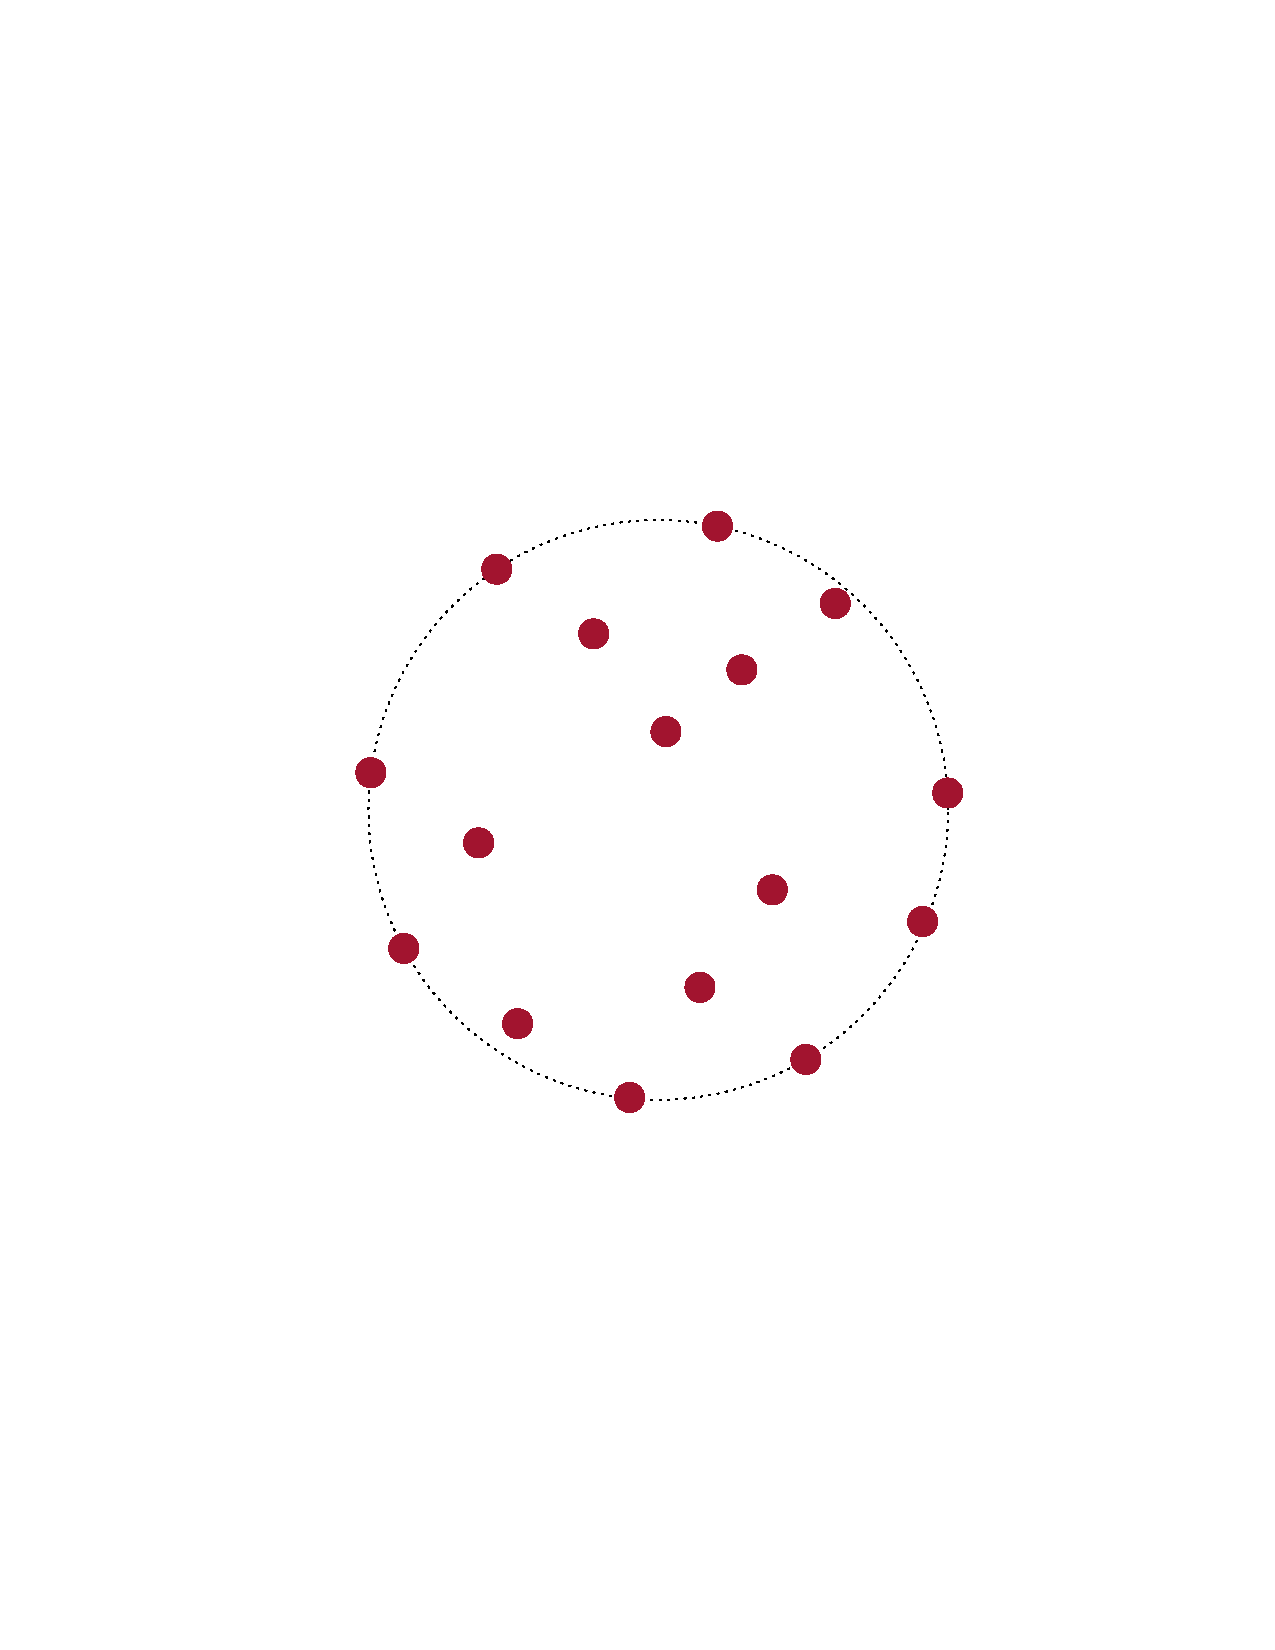
\includegraphics[clip, width=0.3\textwidth, scale=0.025, trim={3cm 8cm 3cm 8cm}]{figures/iea37-opt16-par1.pdf}
	}
	\subfigure[\textit{sub2}]{
		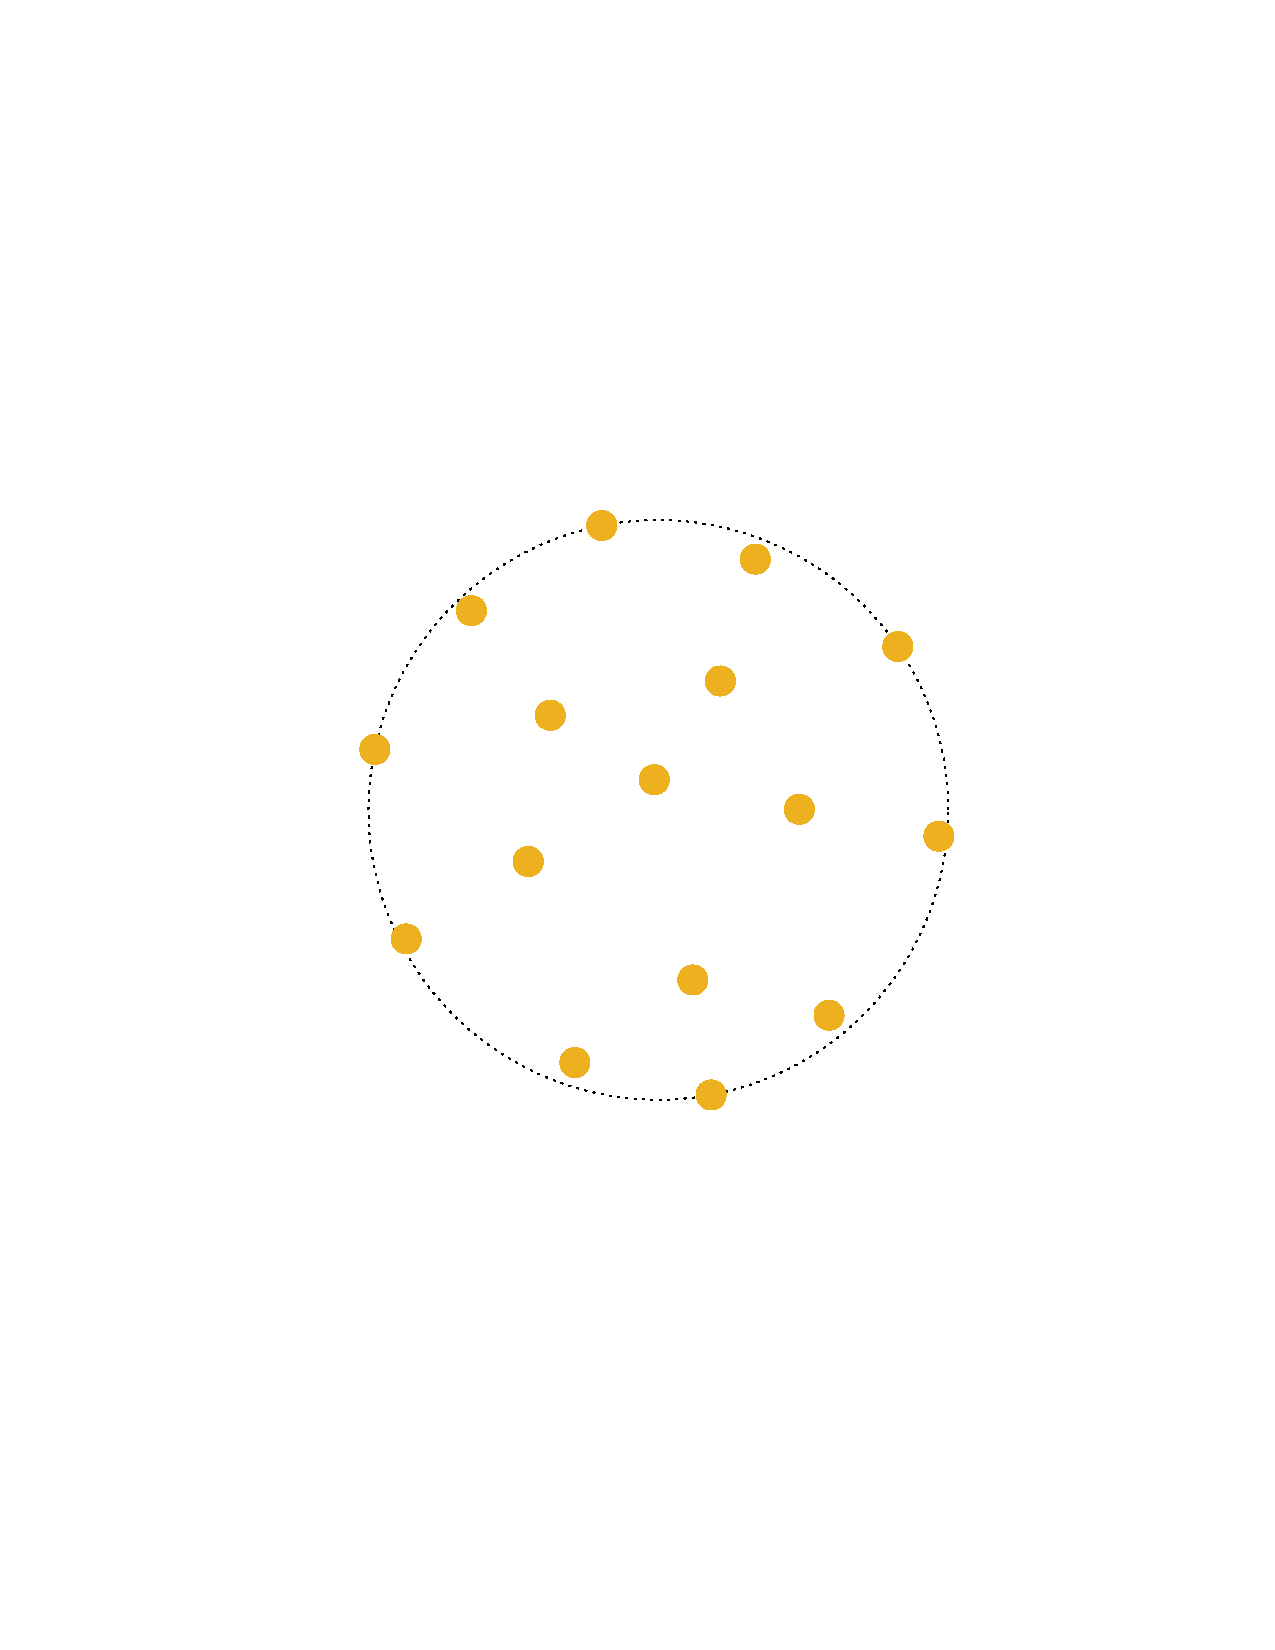
\includegraphics[clip, width=0.3\textwidth,scale=0.025, trim={3cm 8cm 3cm 8cm}]{figures/iea37-opt16-par2.pdf}
	}
	\subfigure[\textit{sub3}]{
		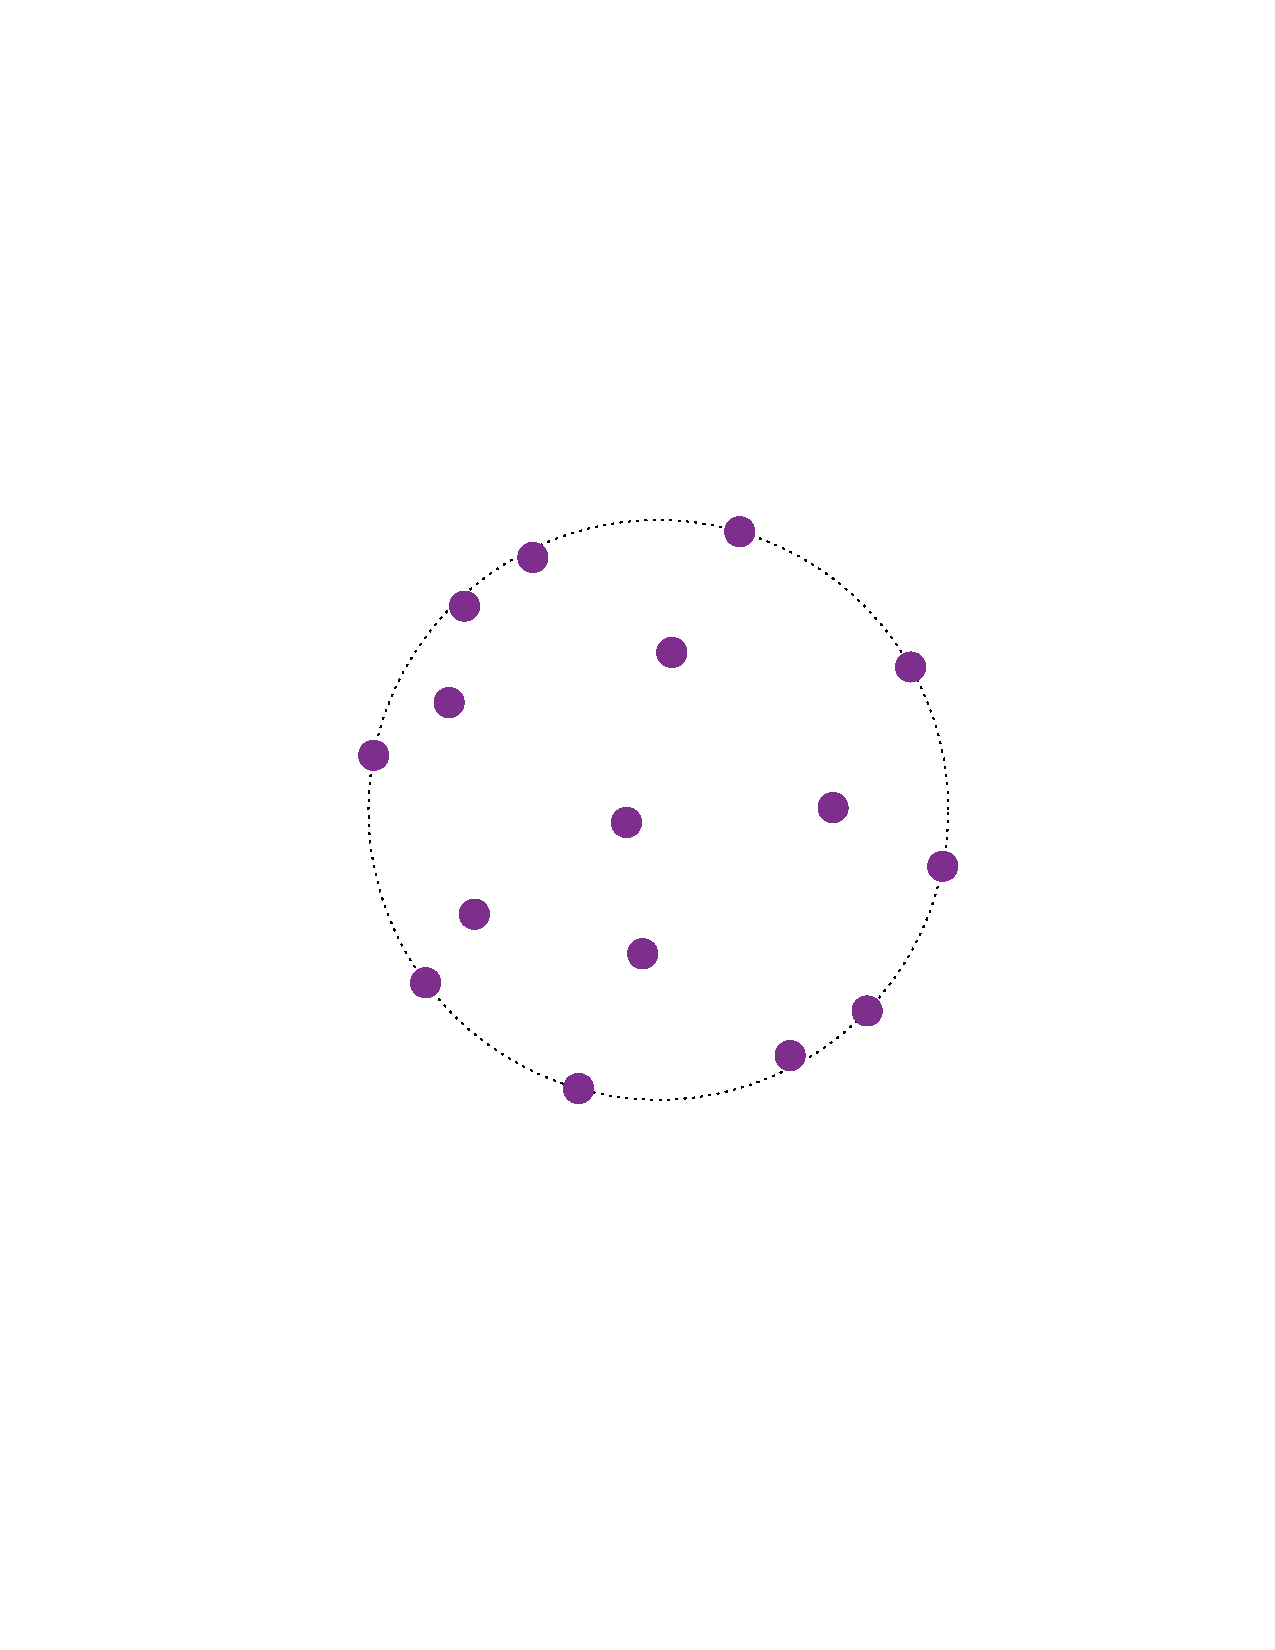
\includegraphics[clip, width=0.3\textwidth,scale=0.025, trim={3cm 8cm 3cm 8cm}]{figures/iea37-opt16-par3.pdf}
	}
	\subfigure[\textit{sub4}]{
		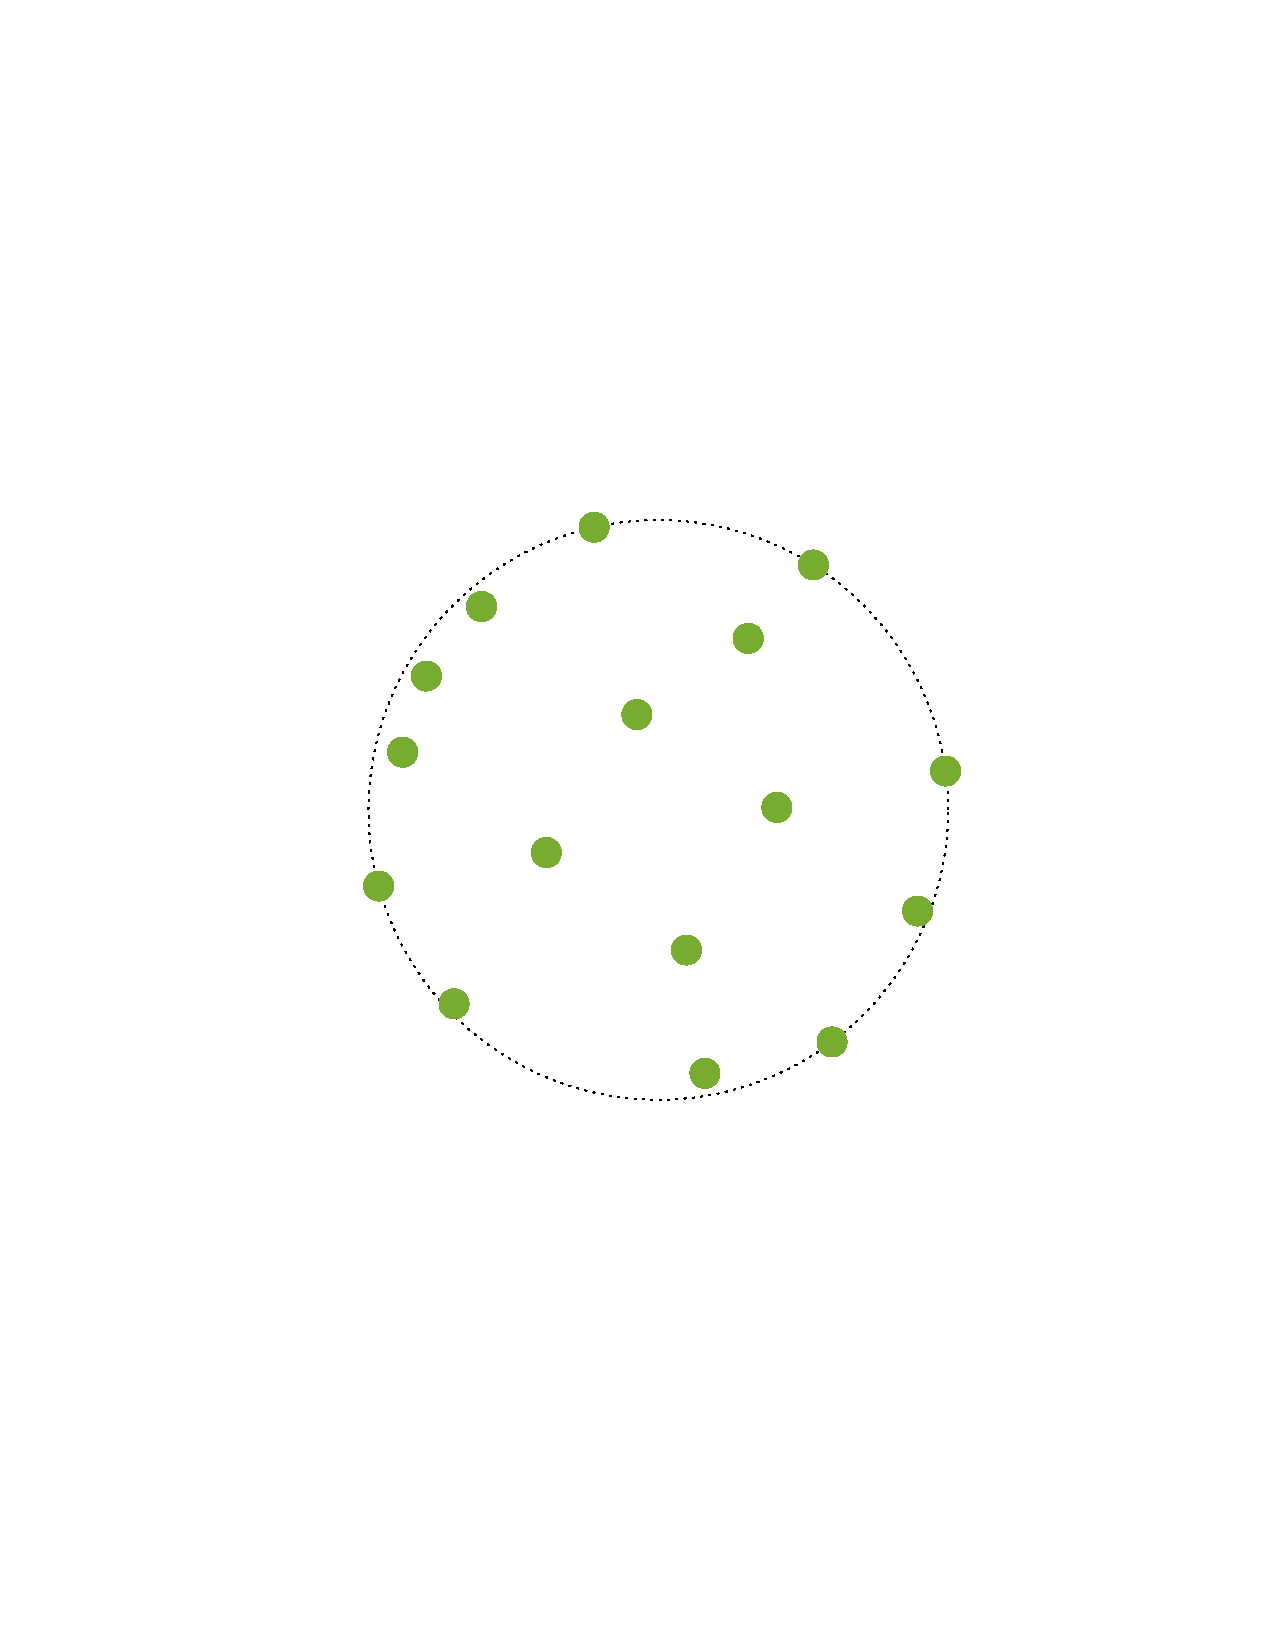
\includegraphics[clip, width=0.3\textwidth, scale=0.025, trim={3cm 8cm 3cm 8cm}]{figures/iea37-opt16-par4.pdf}
	}
	\subfigure[\textit{sub5}]{
		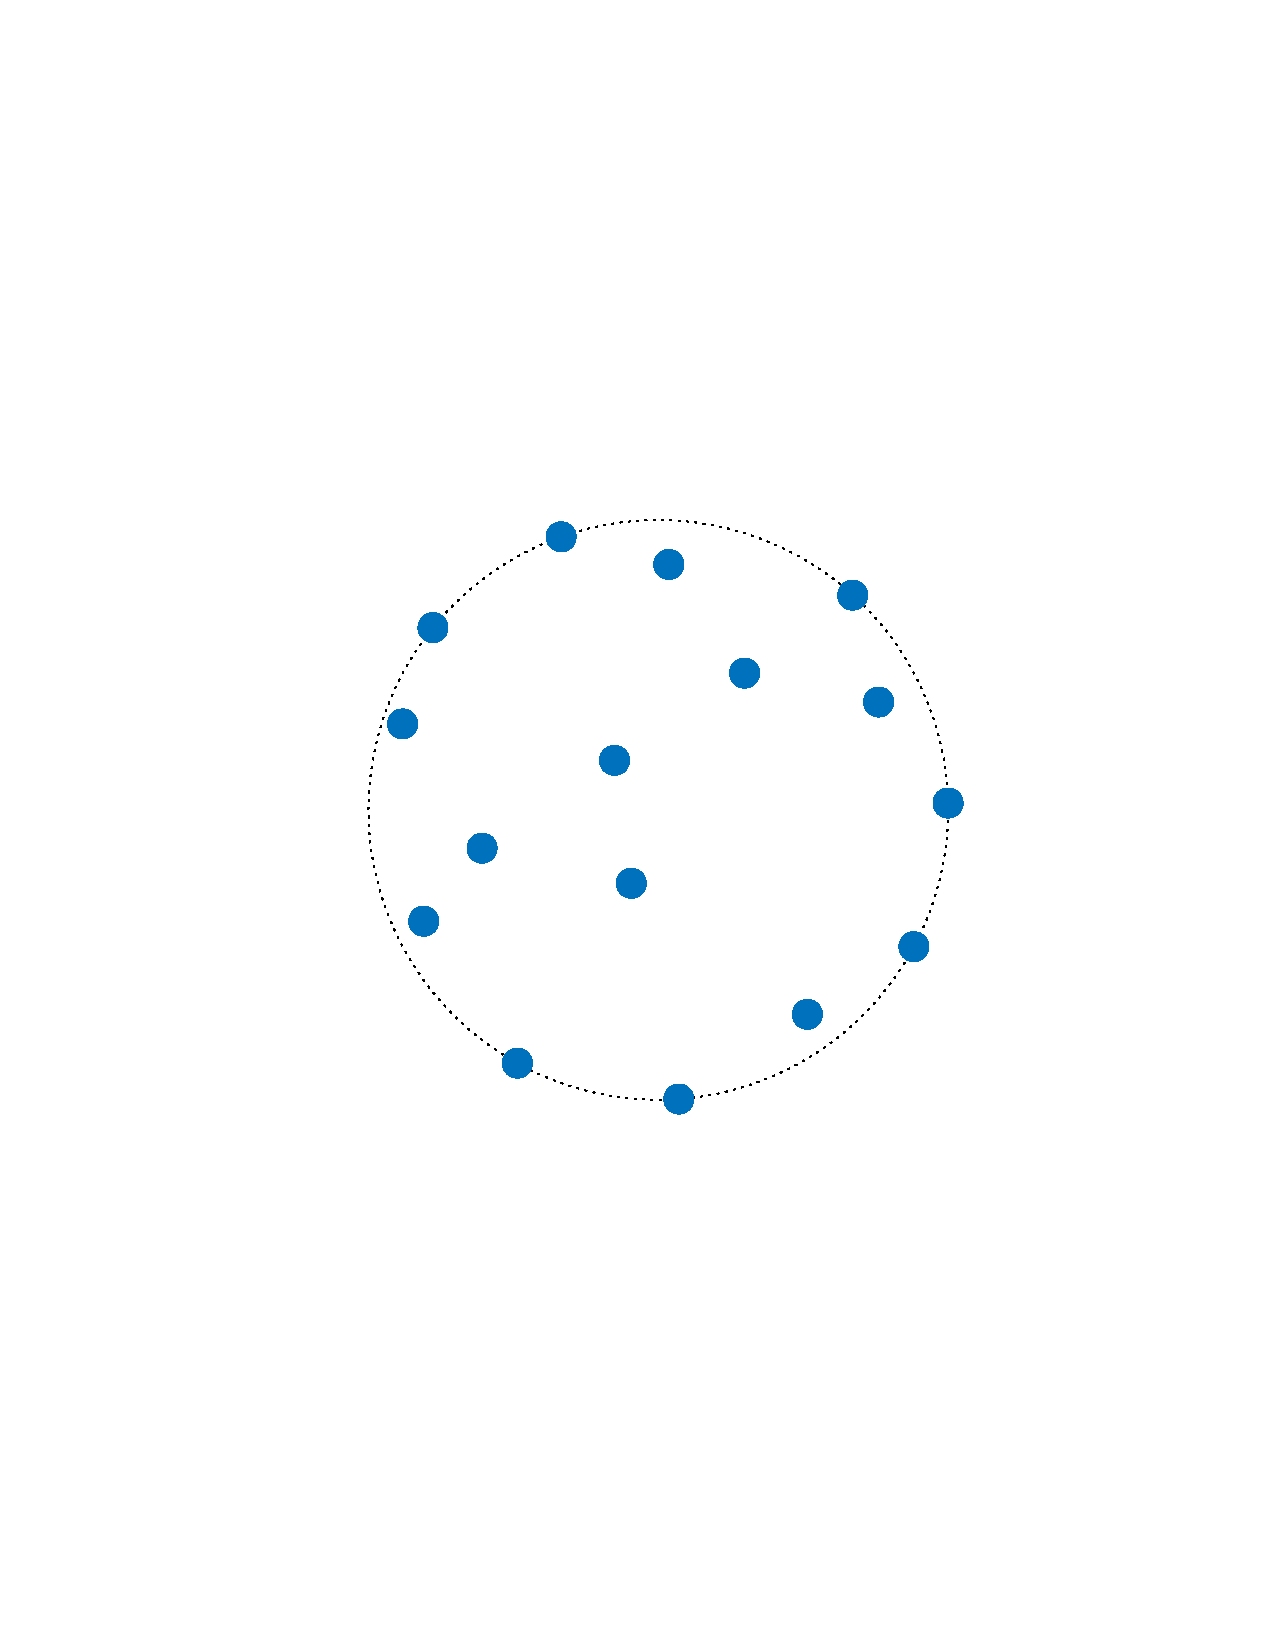
\includegraphics[clip, width=0.3\textwidth, scale=0.025, trim={3cm 8cm 3cm 8cm}]{figures/iea37-opt16-par5.pdf}
	}
	\subfigure[\textit{sub6}]{
		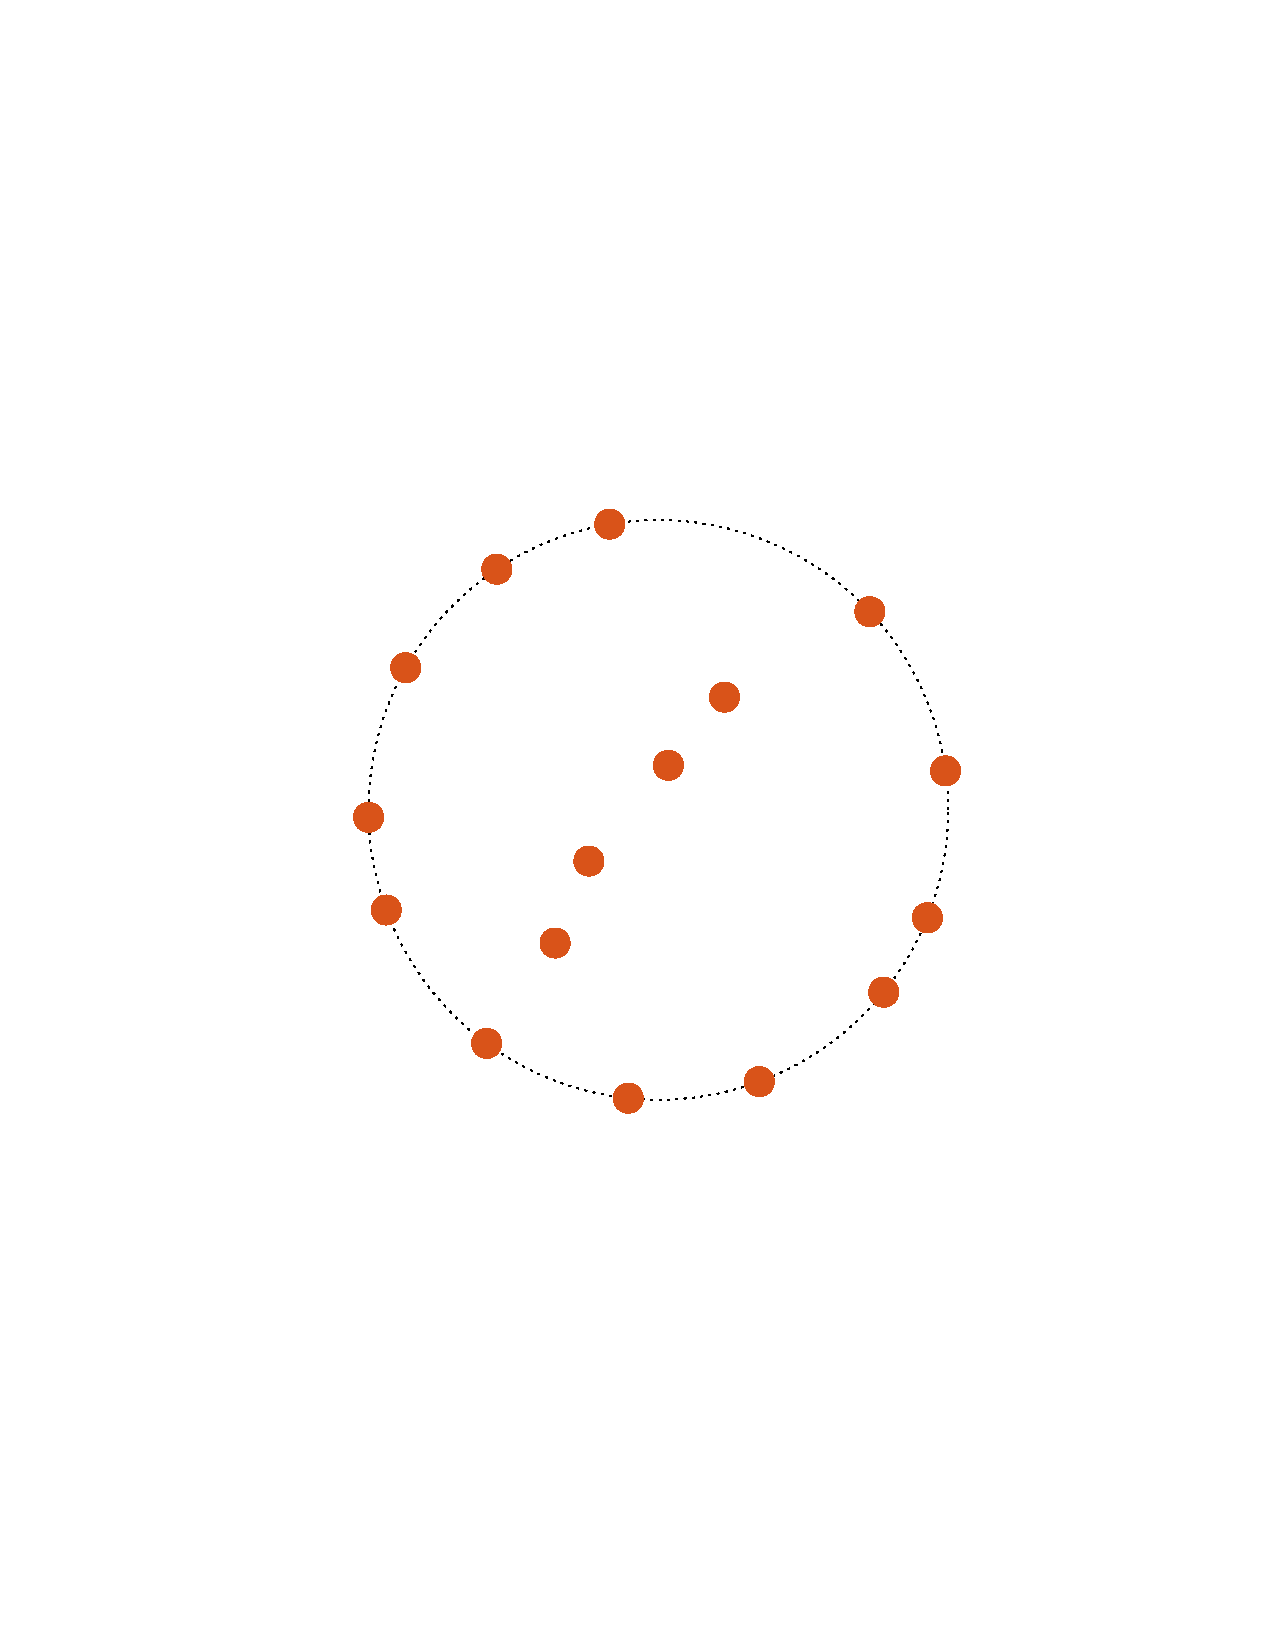
\includegraphics[clip, width=0.3\textwidth, scale=0.025, trim={3cm 8cm 3cm 8cm}]{figures/iea37-opt16-par6.pdf}
	}
	\subfigure[\textit{sub7}]{
		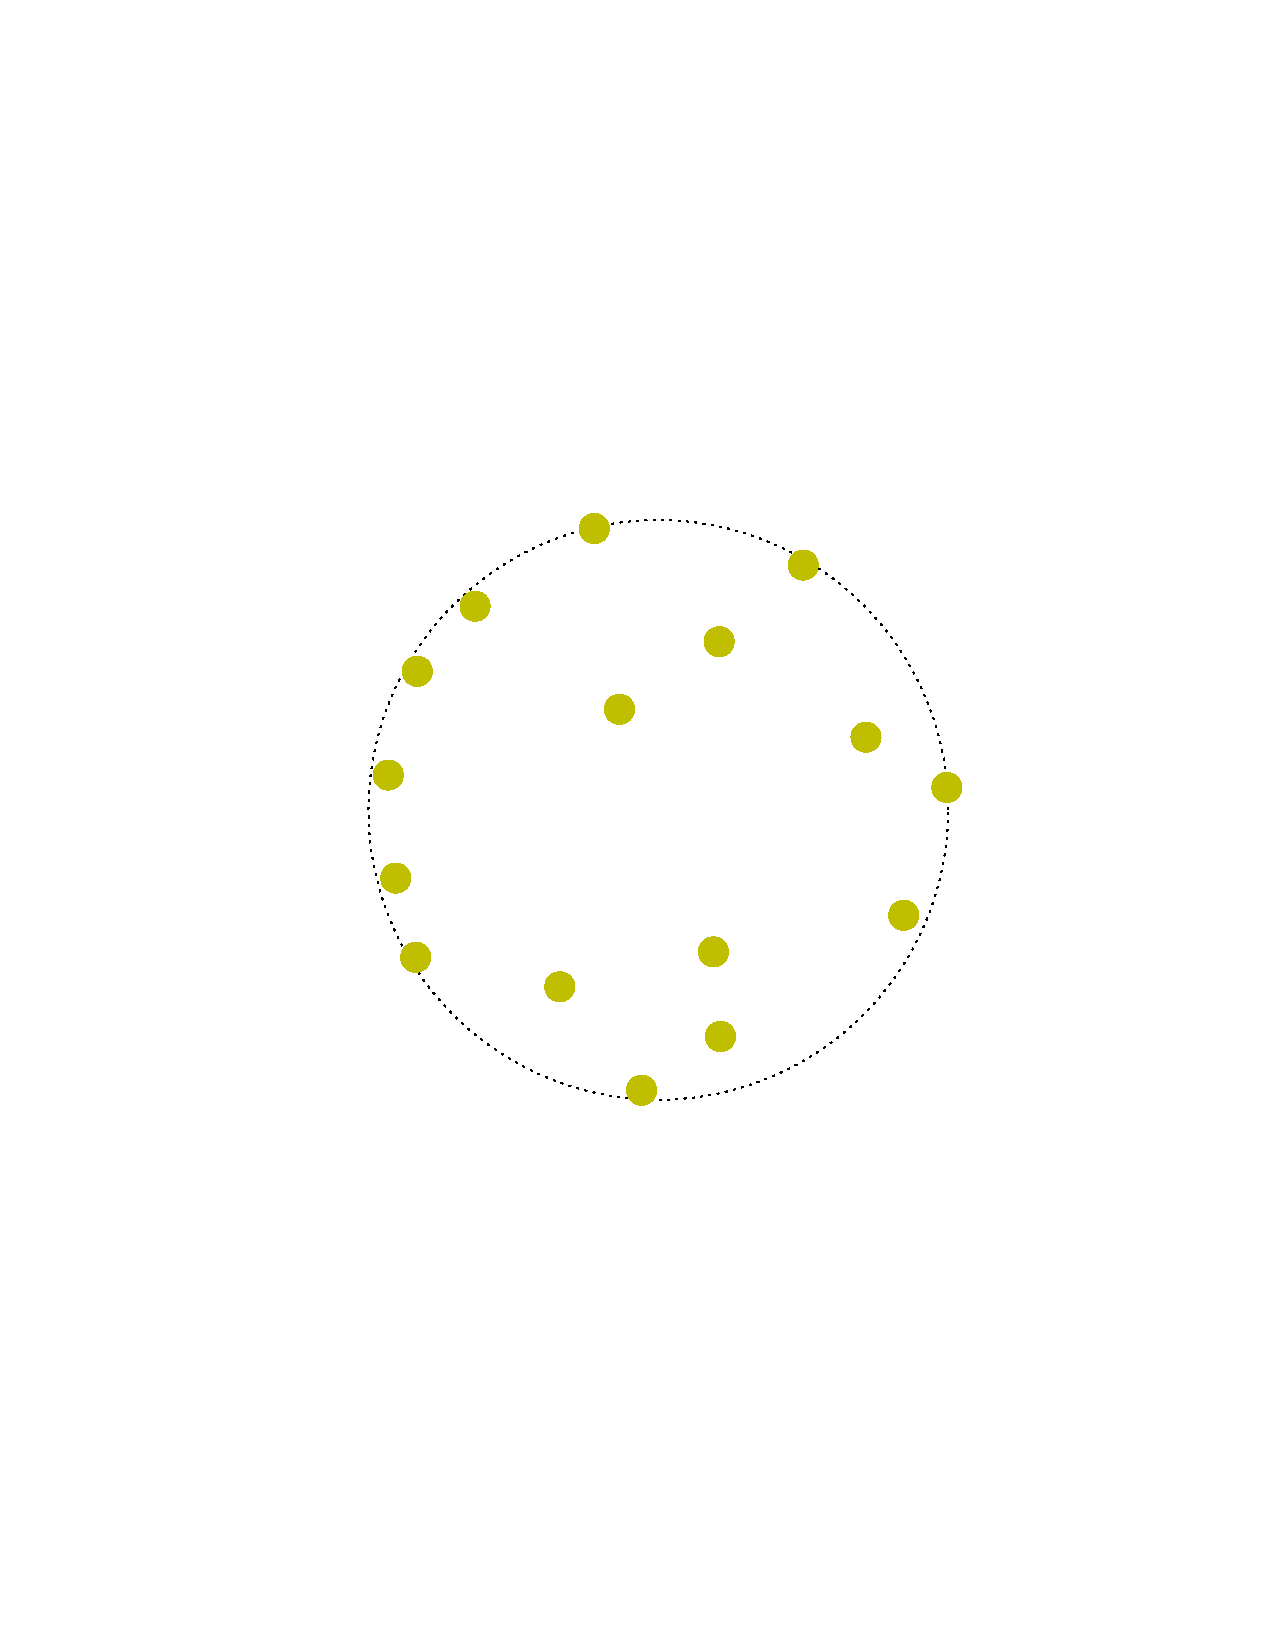
\includegraphics[clip, width=0.3\textwidth,scale=0.025, trim={3cm 8cm 3cm 8cm}]{figures/iea37-opt16-par7.pdf}
	}
	\subfigure[\textit{sub8}]{
		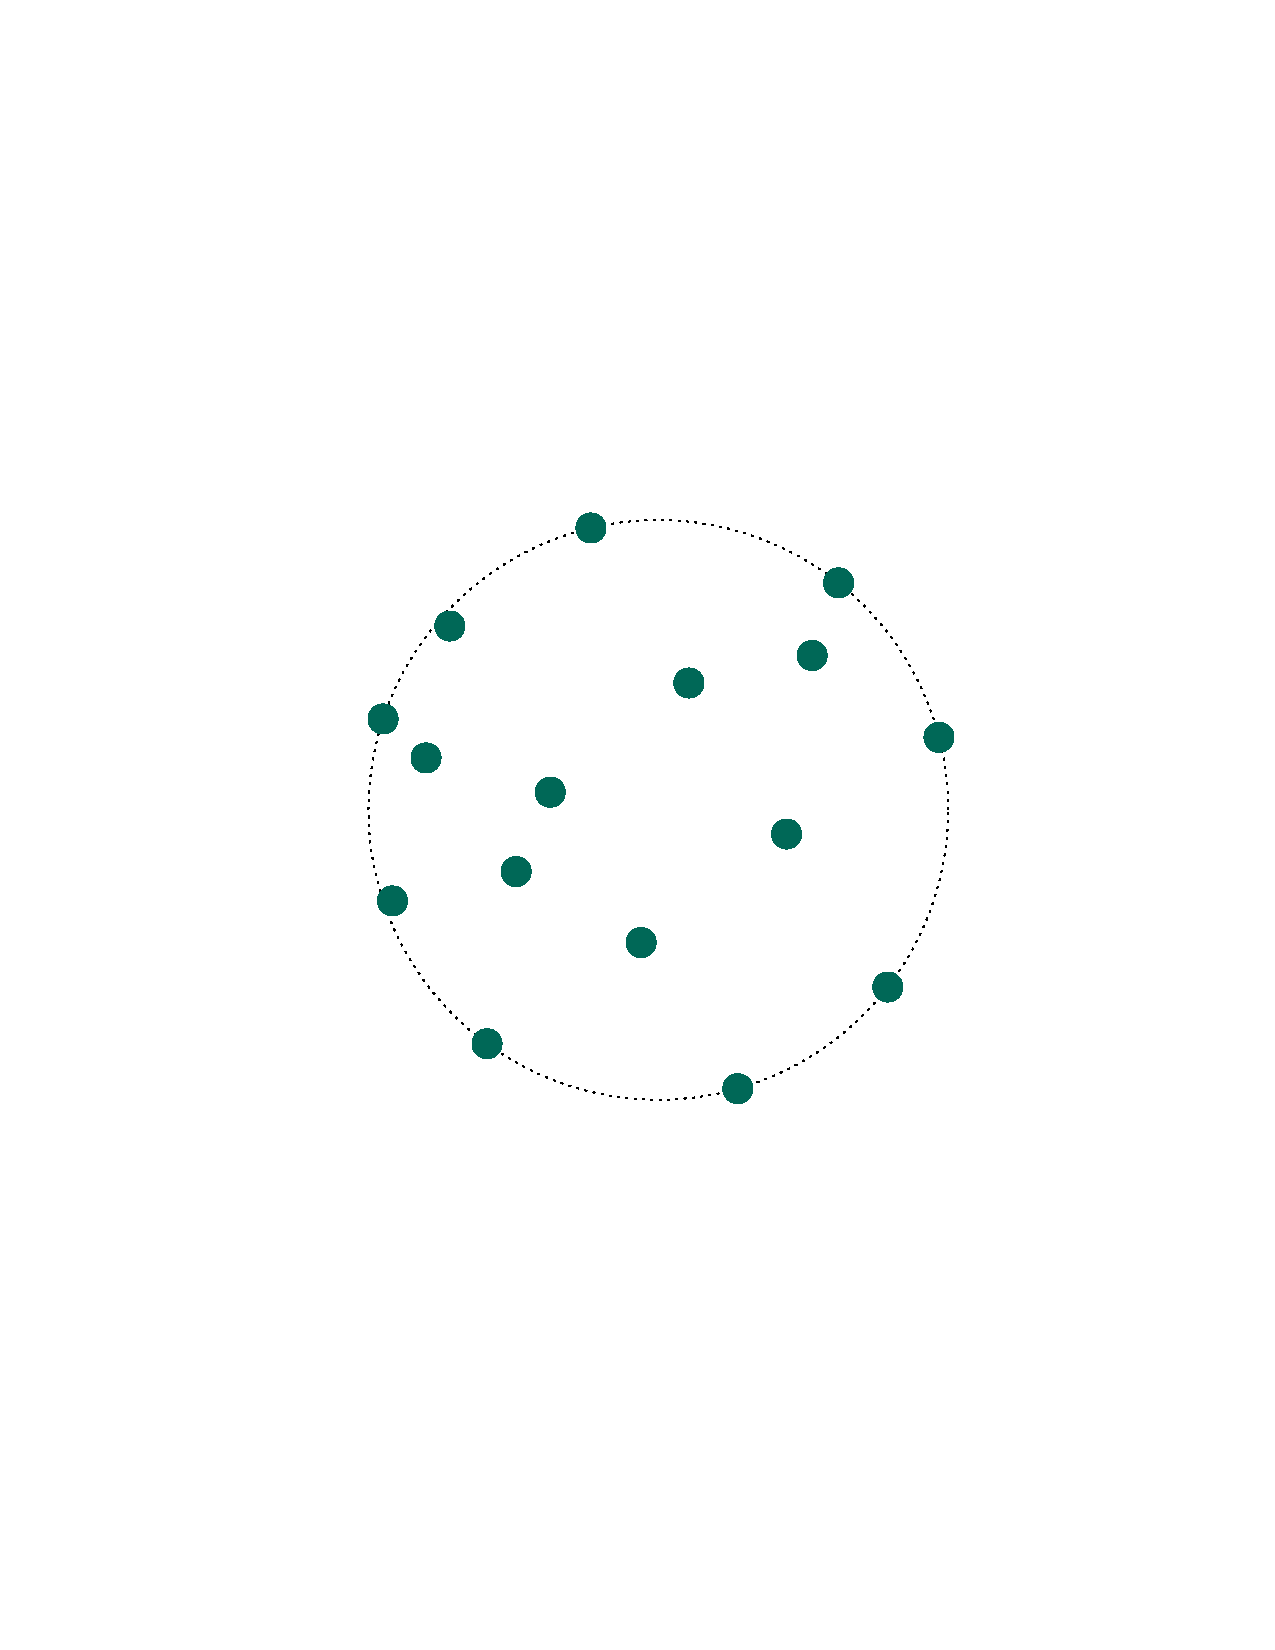
\includegraphics[clip, width=0.3\textwidth,scale=0.025, trim={3cm 8cm 3cm 8cm}]{figures/iea37-opt16-par8.pdf}
	}
	\subfigure[\textit{sub9}]{
		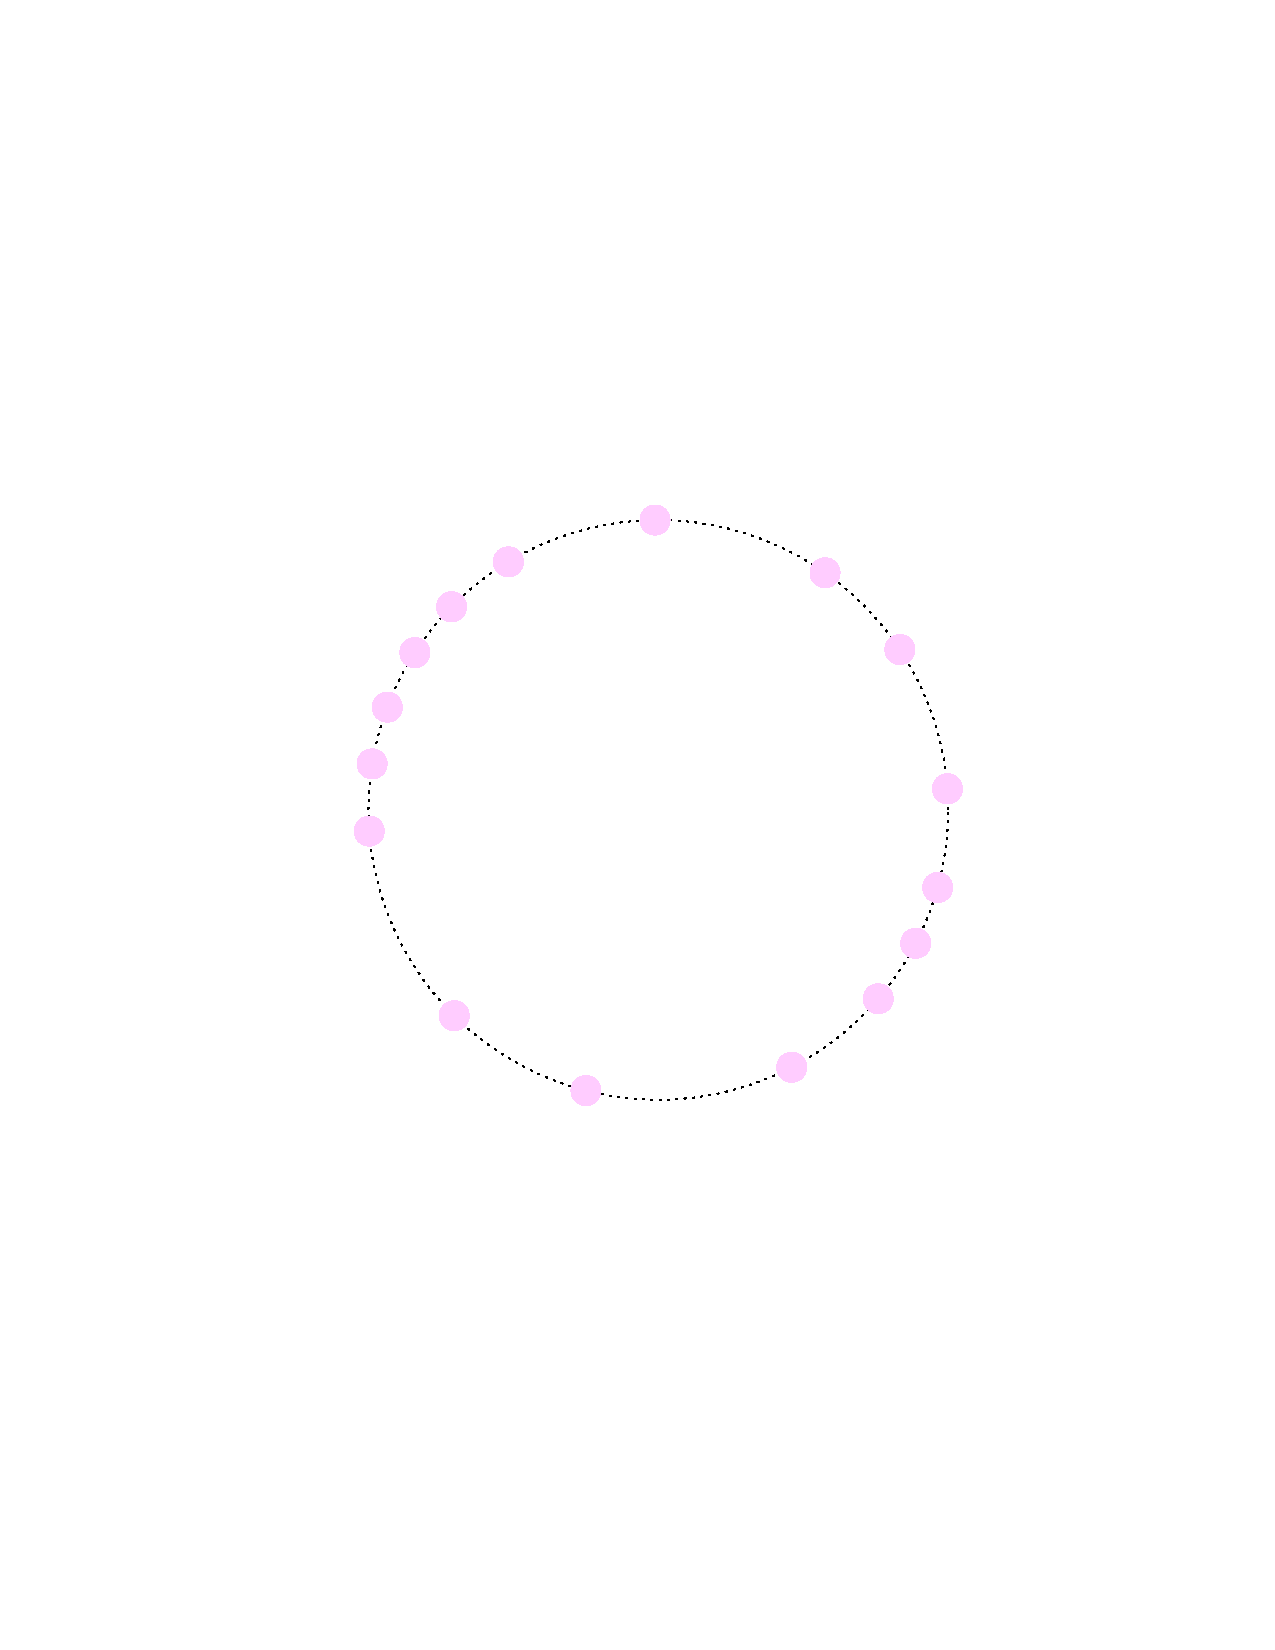
\includegraphics[clip, width=0.3\textwidth, scale=0.025, trim={3cm 8cm 3cm 8cm}]{figures/iea37-opt16-par9.pdf}
	}
	\subfigure[\textit{sub10}]{
		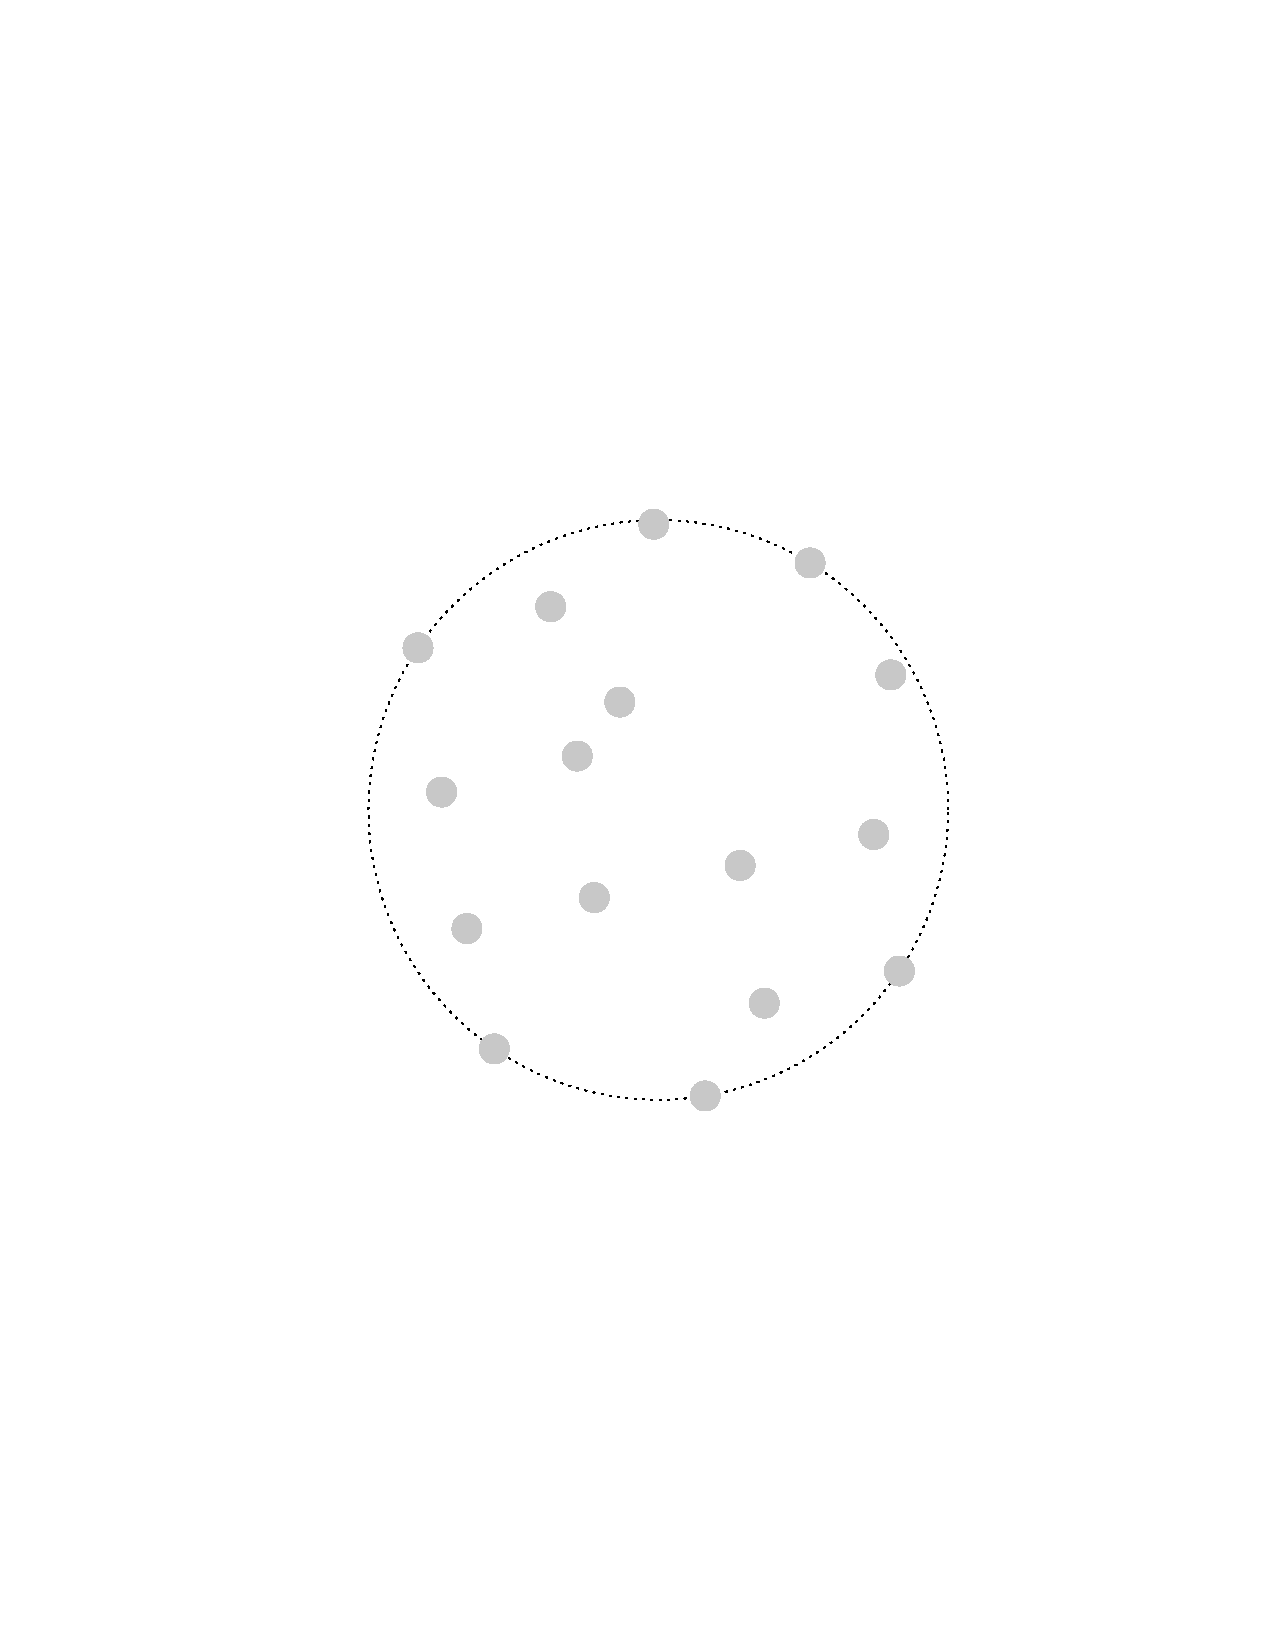
\includegraphics[clip, width=0.3\textwidth, scale=0.025, trim={3cm 8cm 3cm 8cm}]{figures/iea37-opt16-par10.pdf}
	}
	\caption{Case study 1: optimized wind farm layouts with 16 wind turbines.}
	\label{fig:16turbs}
\end{figure}

\begin{figure}[htbp!]
	\centering
	\subfigure[\textit{sub1}]{
		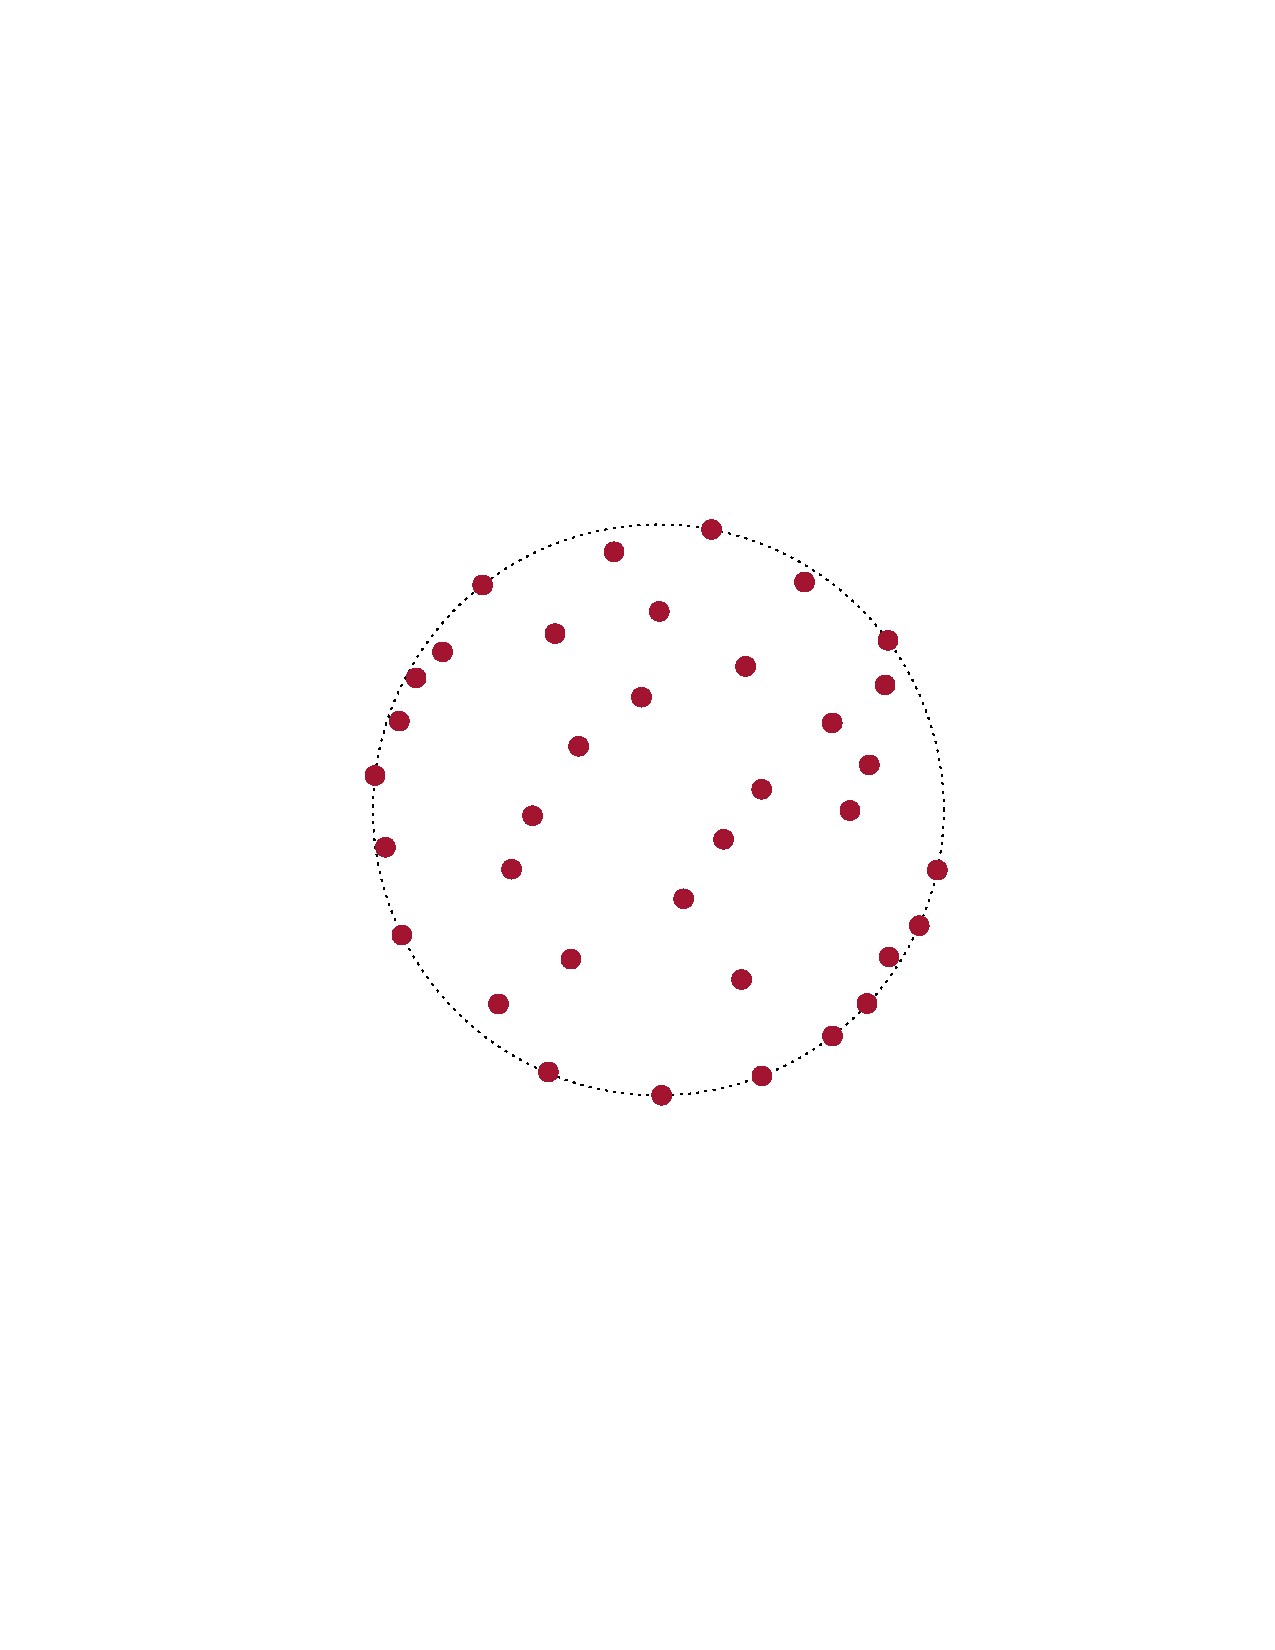
\includegraphics[clip, width=0.3\textwidth, scale=0.025, trim={3cm 8cm 3cm 8cm}]{figures/iea37-opt36-par1.pdf}
	}
	\subfigure[\textit{sub2}]{
		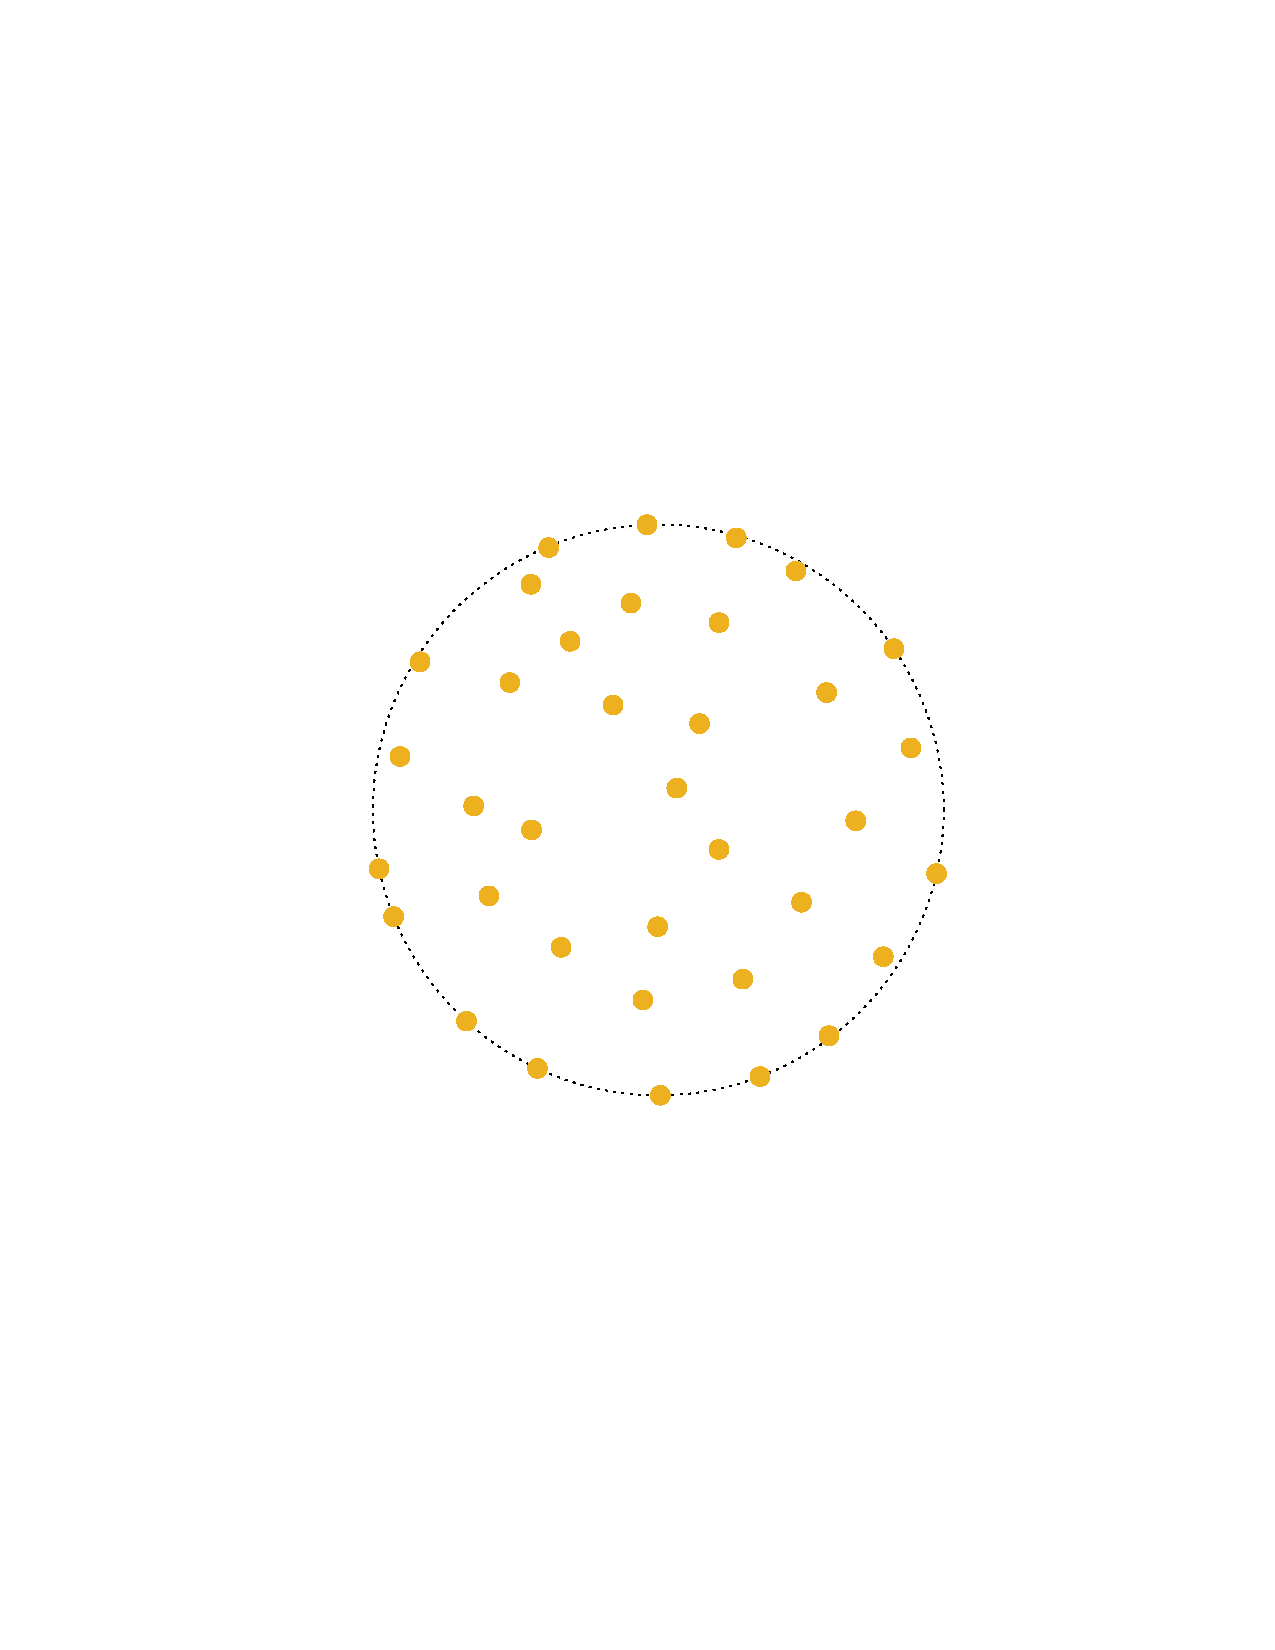
\includegraphics[clip, width=0.3\textwidth,scale=0.025, trim={3cm 8cm 3cm 8cm}]{figures/iea37-opt36-par2.pdf}
	}
	\subfigure[\textit{sub3}]{
		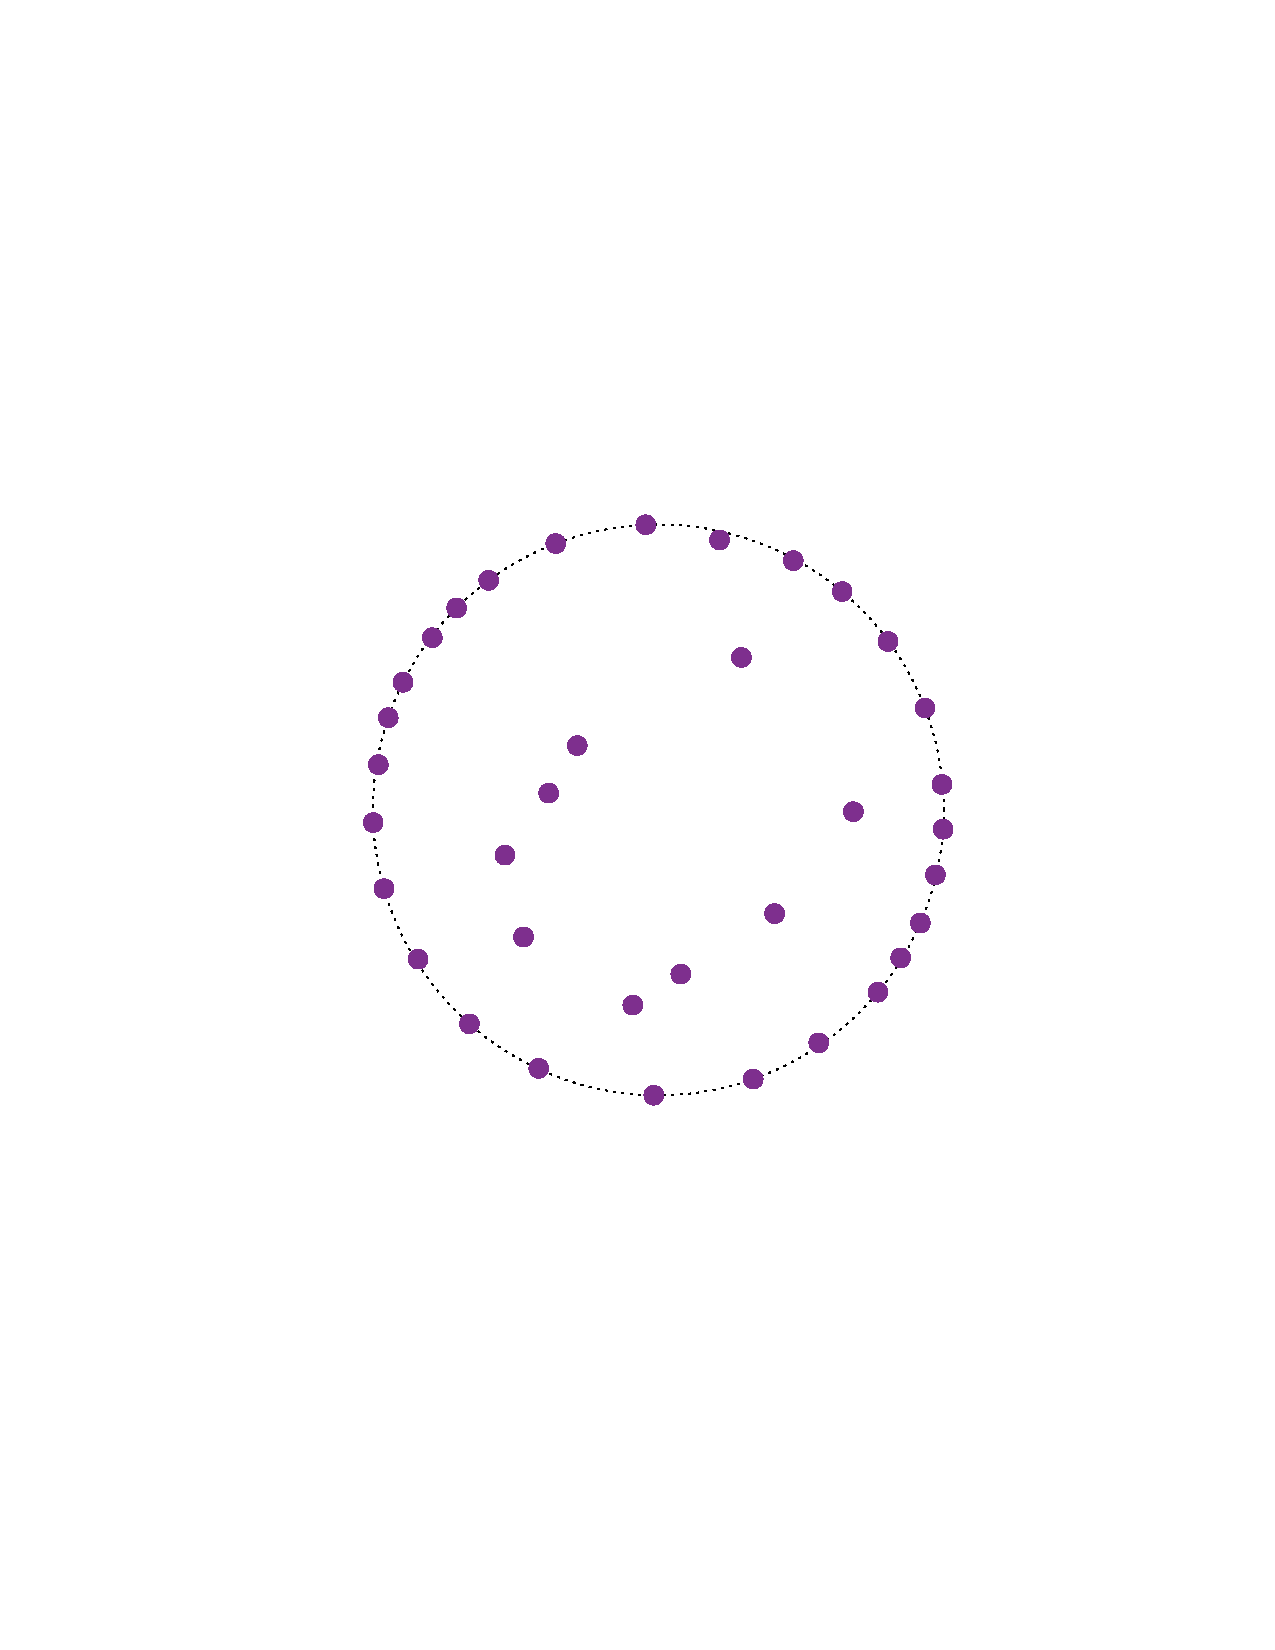
\includegraphics[clip, width=0.3\textwidth,scale=0.025, trim={3cm 8cm 3cm 8cm}]{figures/iea37-opt36-par3.pdf}
	}
	\subfigure[\textit{sub4}]{
		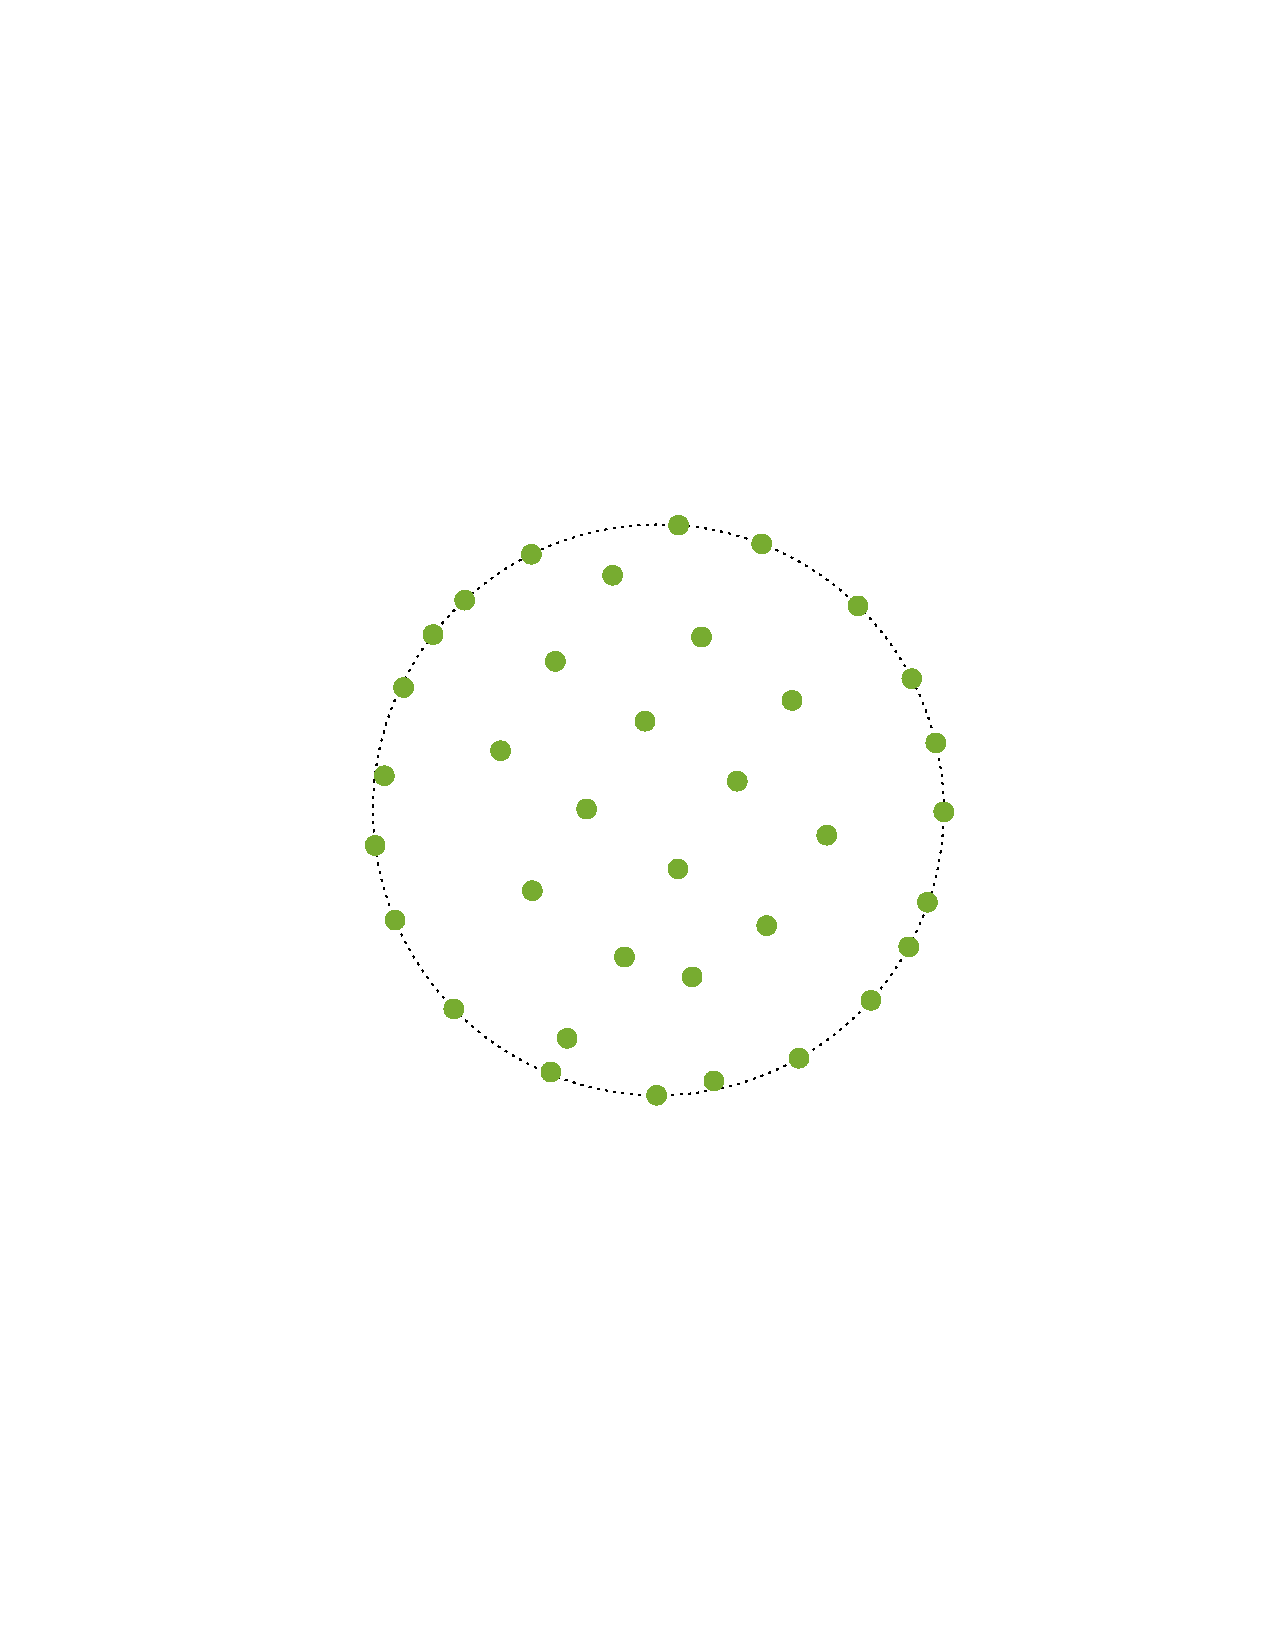
\includegraphics[clip, width=0.3\textwidth, scale=0.025, trim={3cm 8cm 3cm 8cm}]{figures/iea37-opt36-par4.pdf}
	}
	\subfigure[\textit{sub5}]{
		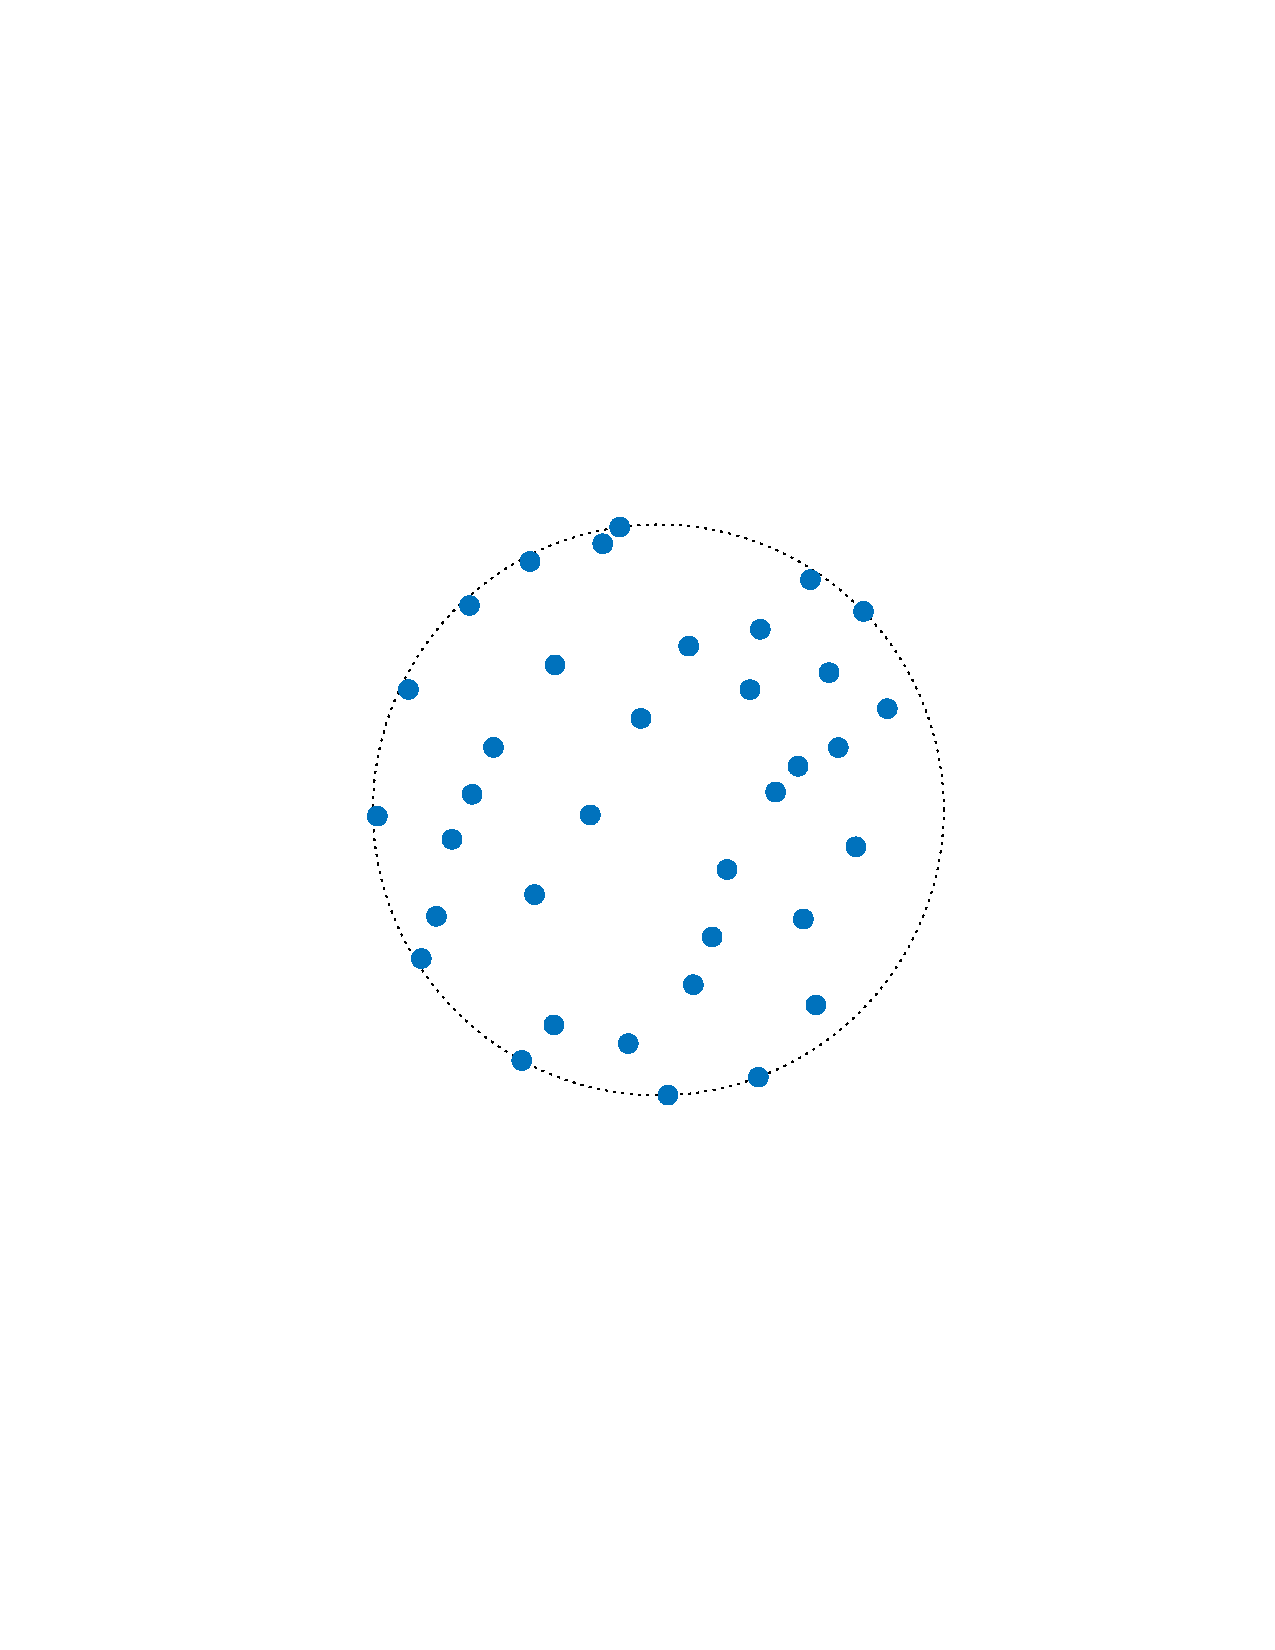
\includegraphics[clip, width=0.3\textwidth, scale=0.025, trim={3cm 8cm 3cm 8cm}]{figures/iea37-opt36-par5.pdf}
	}
	\subfigure[\textit{sub6}]{
		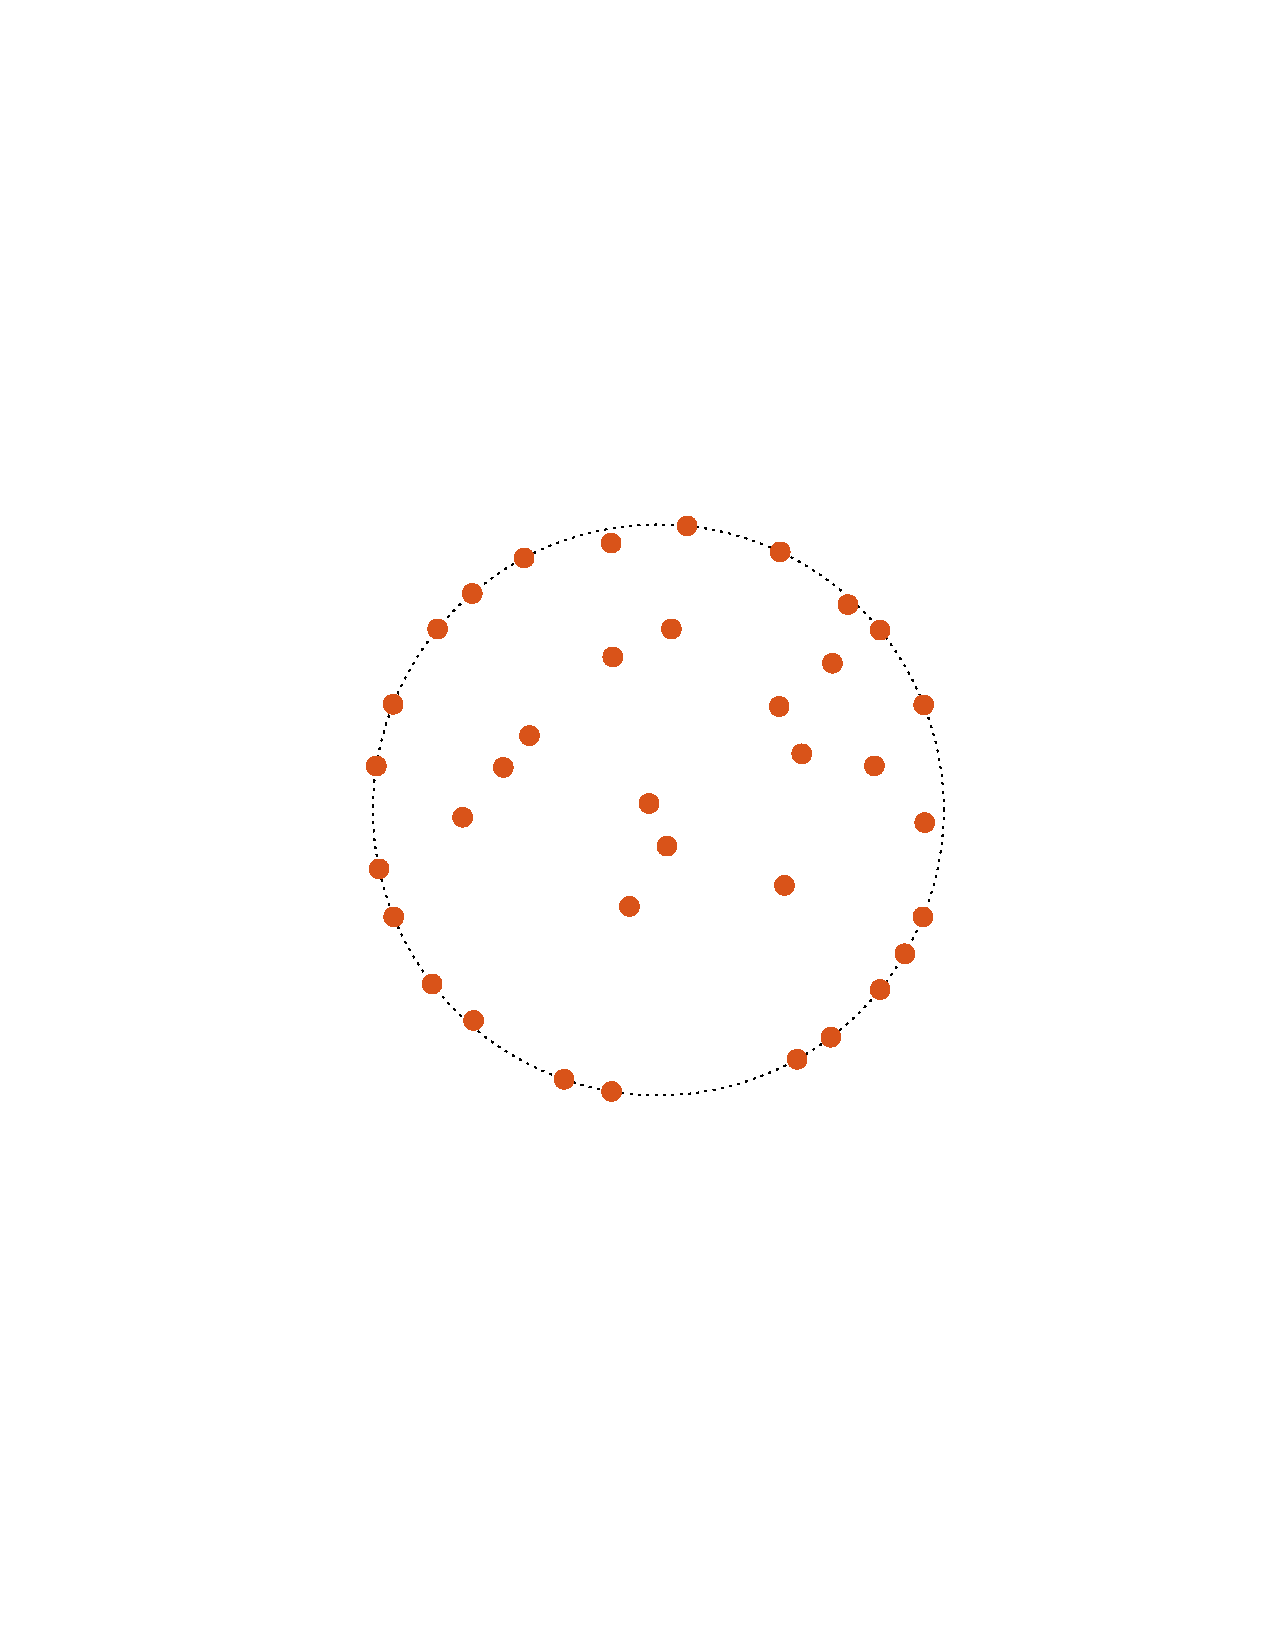
\includegraphics[clip, width=0.3\textwidth, scale=0.025, trim={3cm 8cm 3cm 8cm}]{figures/iea37-opt36-par6.pdf}
	}
	\subfigure[\textit{sub7}]{
		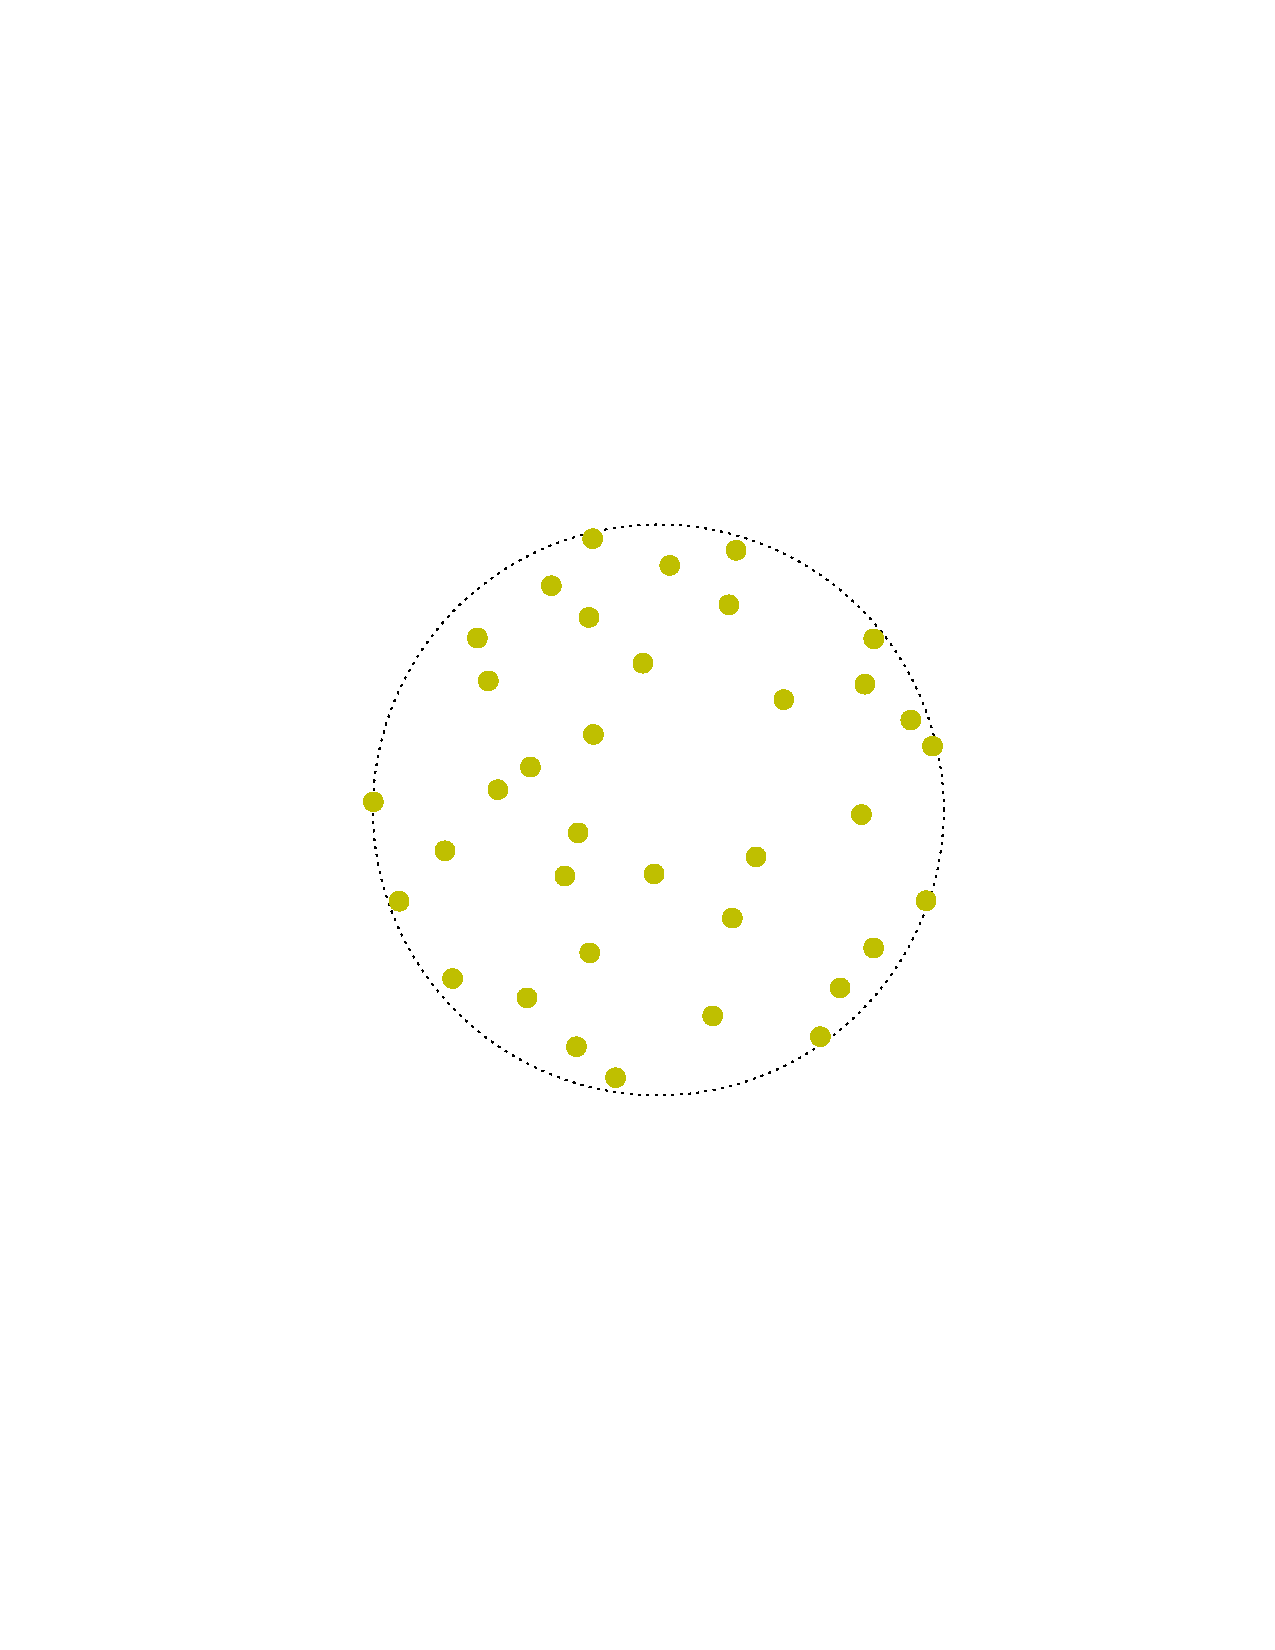
\includegraphics[clip, width=0.3\textwidth,scale=0.025, trim={3cm 8cm 3cm 8cm}]{figures/iea37-opt36-par7.pdf}
	}
	\subfigure[\textit{sub8}]{
		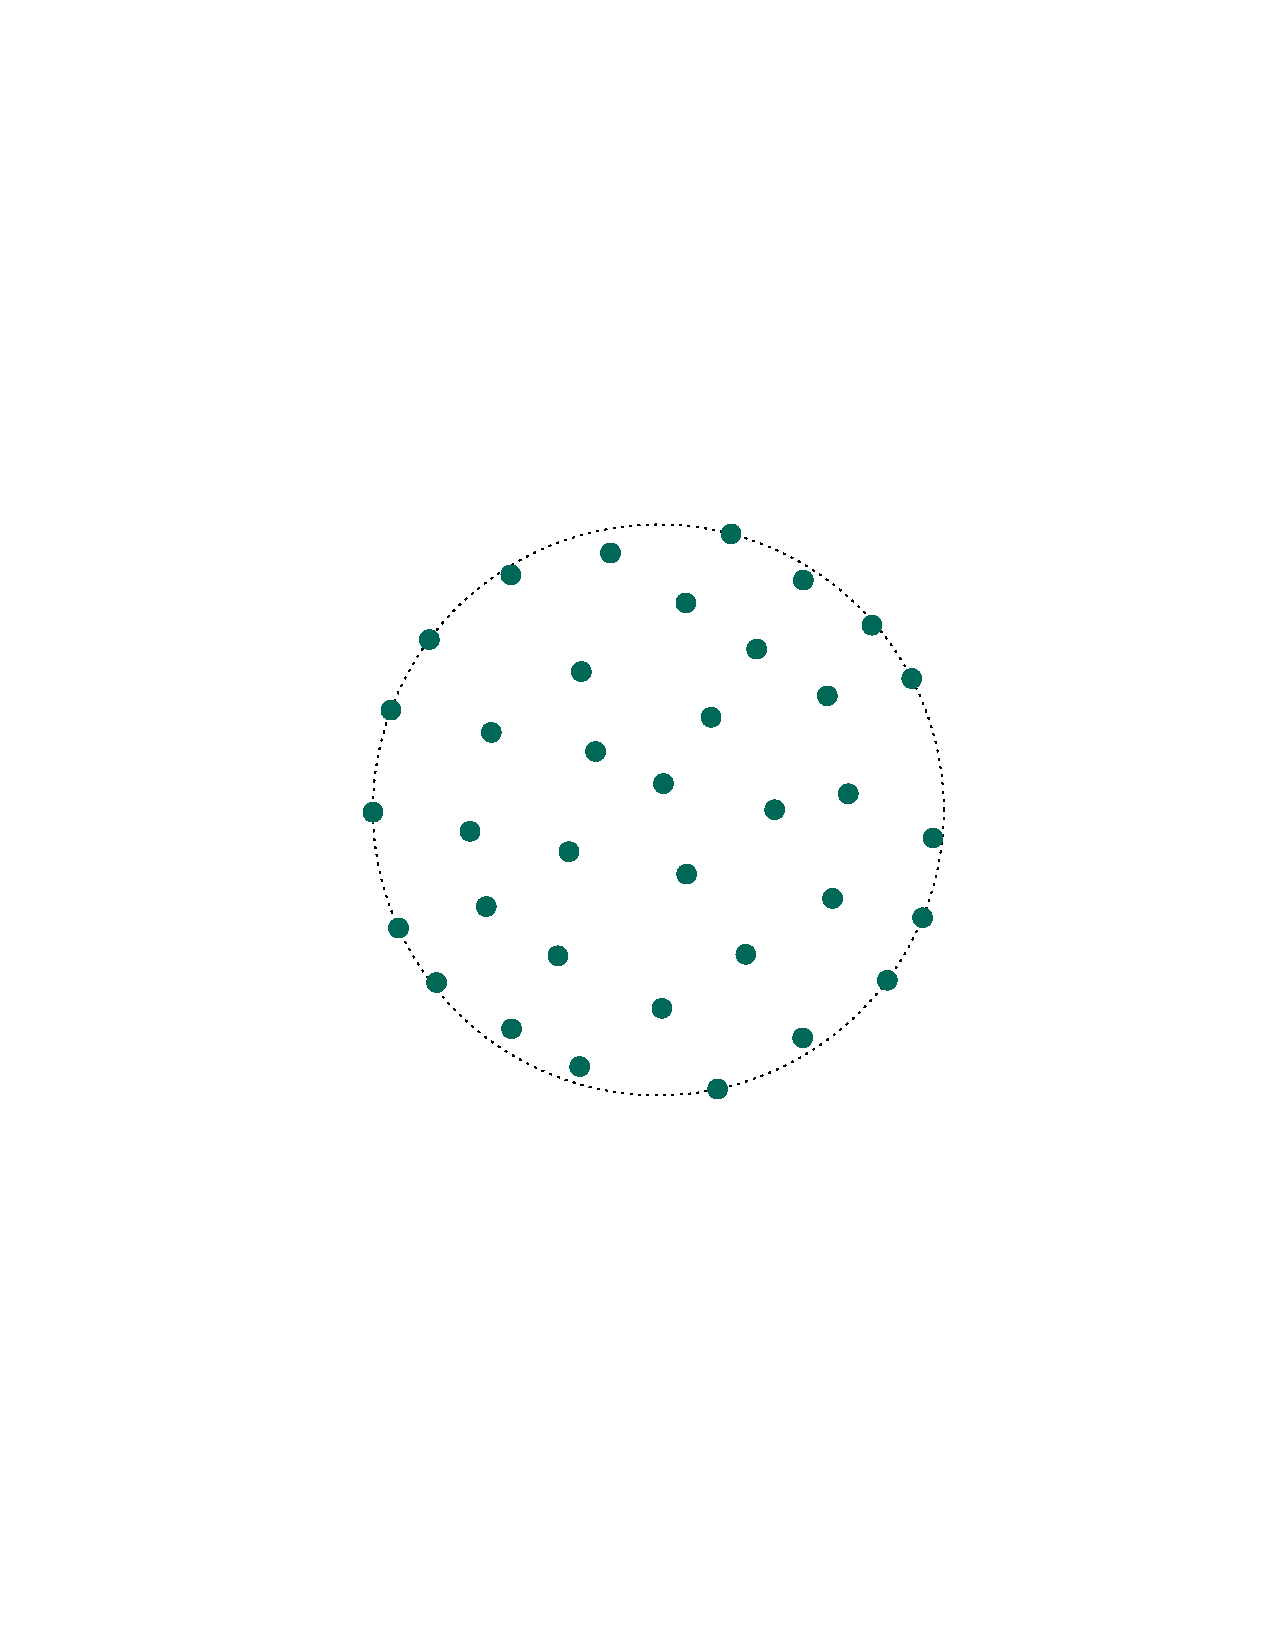
\includegraphics[clip, width=0.3\textwidth,scale=0.025, trim={3cm 8cm 3cm 8cm}]{figures/iea37-opt36-par8.pdf}
	}
	\subfigure[\textit{sub9}]{
		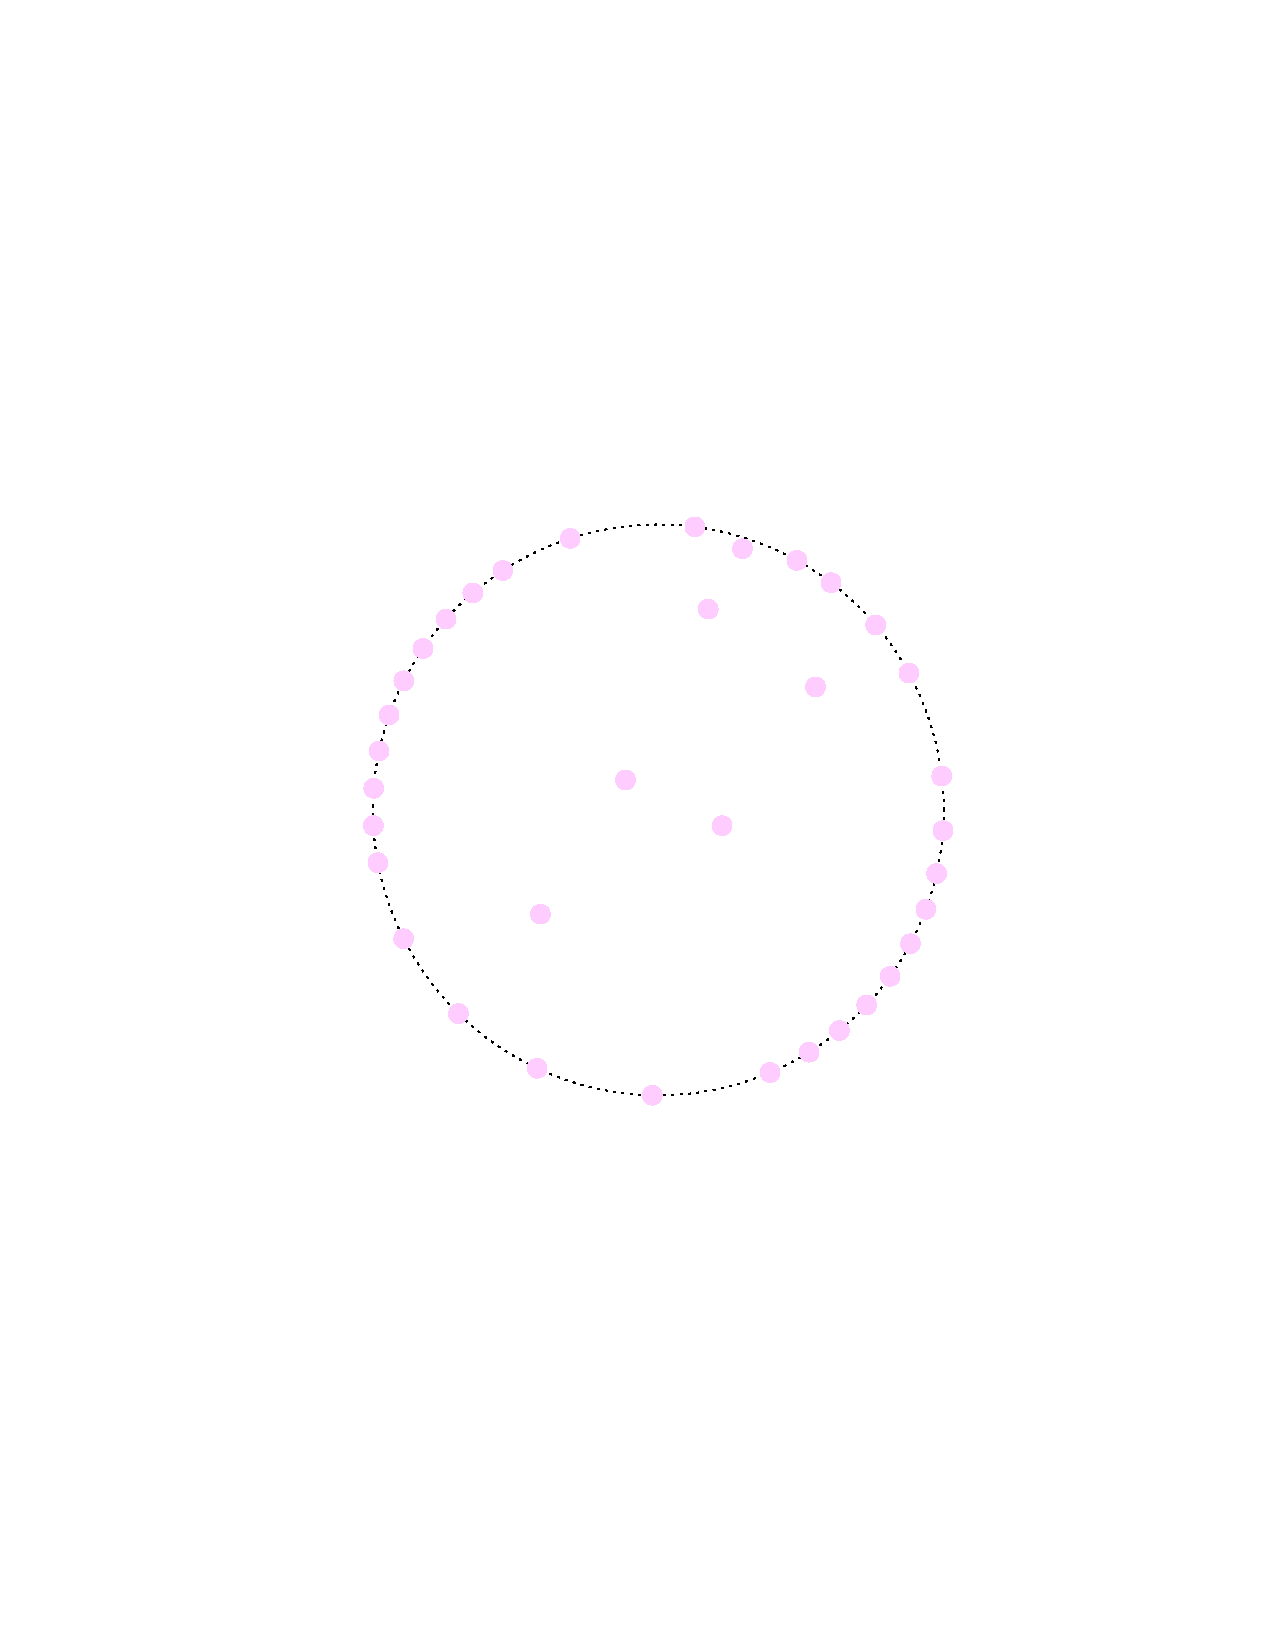
\includegraphics[clip, width=0.3\textwidth, scale=0.025, trim={3cm 8cm 3cm 8cm}]{figures/iea37-opt36-par9.pdf}
	}
	\subfigure[\textit{sub10}]{
		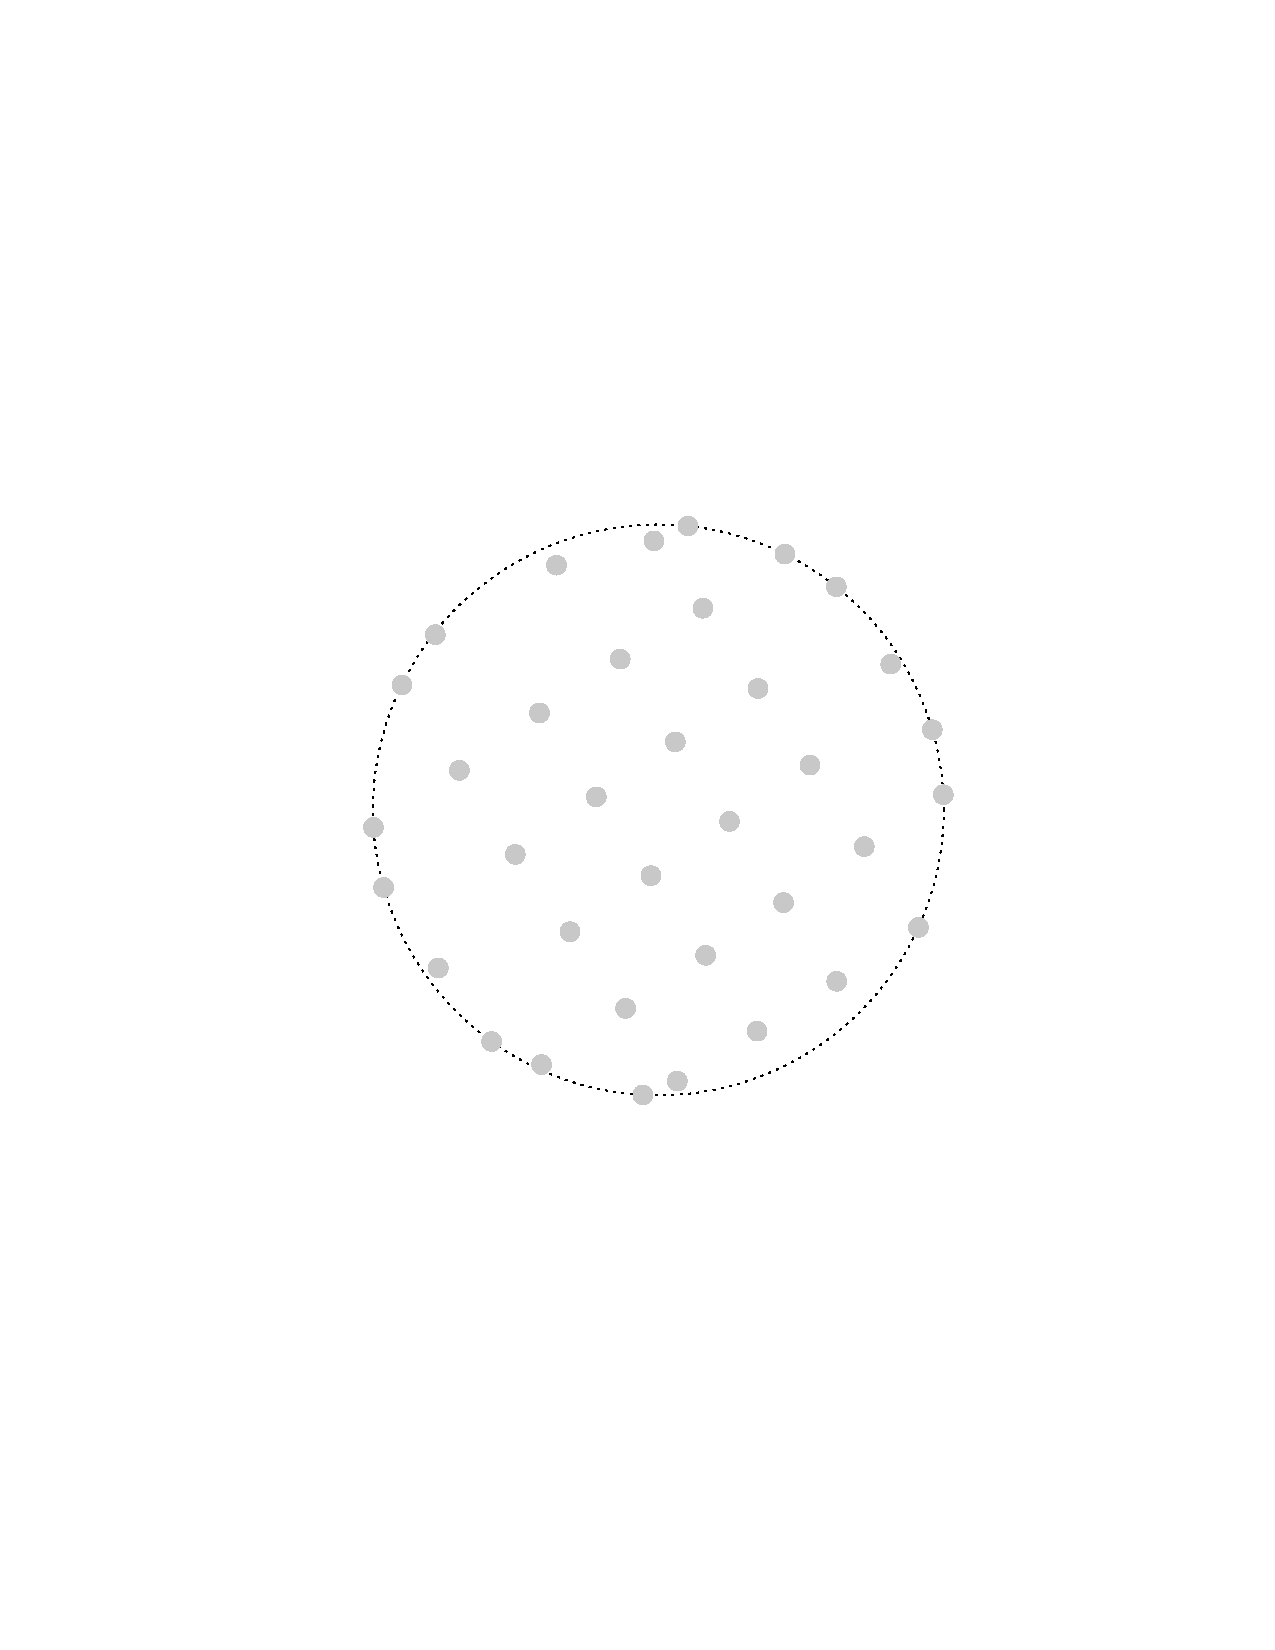
\includegraphics[clip, width=0.3\textwidth, scale=0.025, trim={3cm 8cm 3cm 8cm}]{figures/iea37-opt36-par10.pdf}
	}
	\caption{Case study 1: optimized wind farm layouts with 36 wind turbines.}
	\label{fig:36turbs}
\end{figure}

\begin{figure}[htbp!]
	\centering
	\subfigure[\textit{sub1}]{
		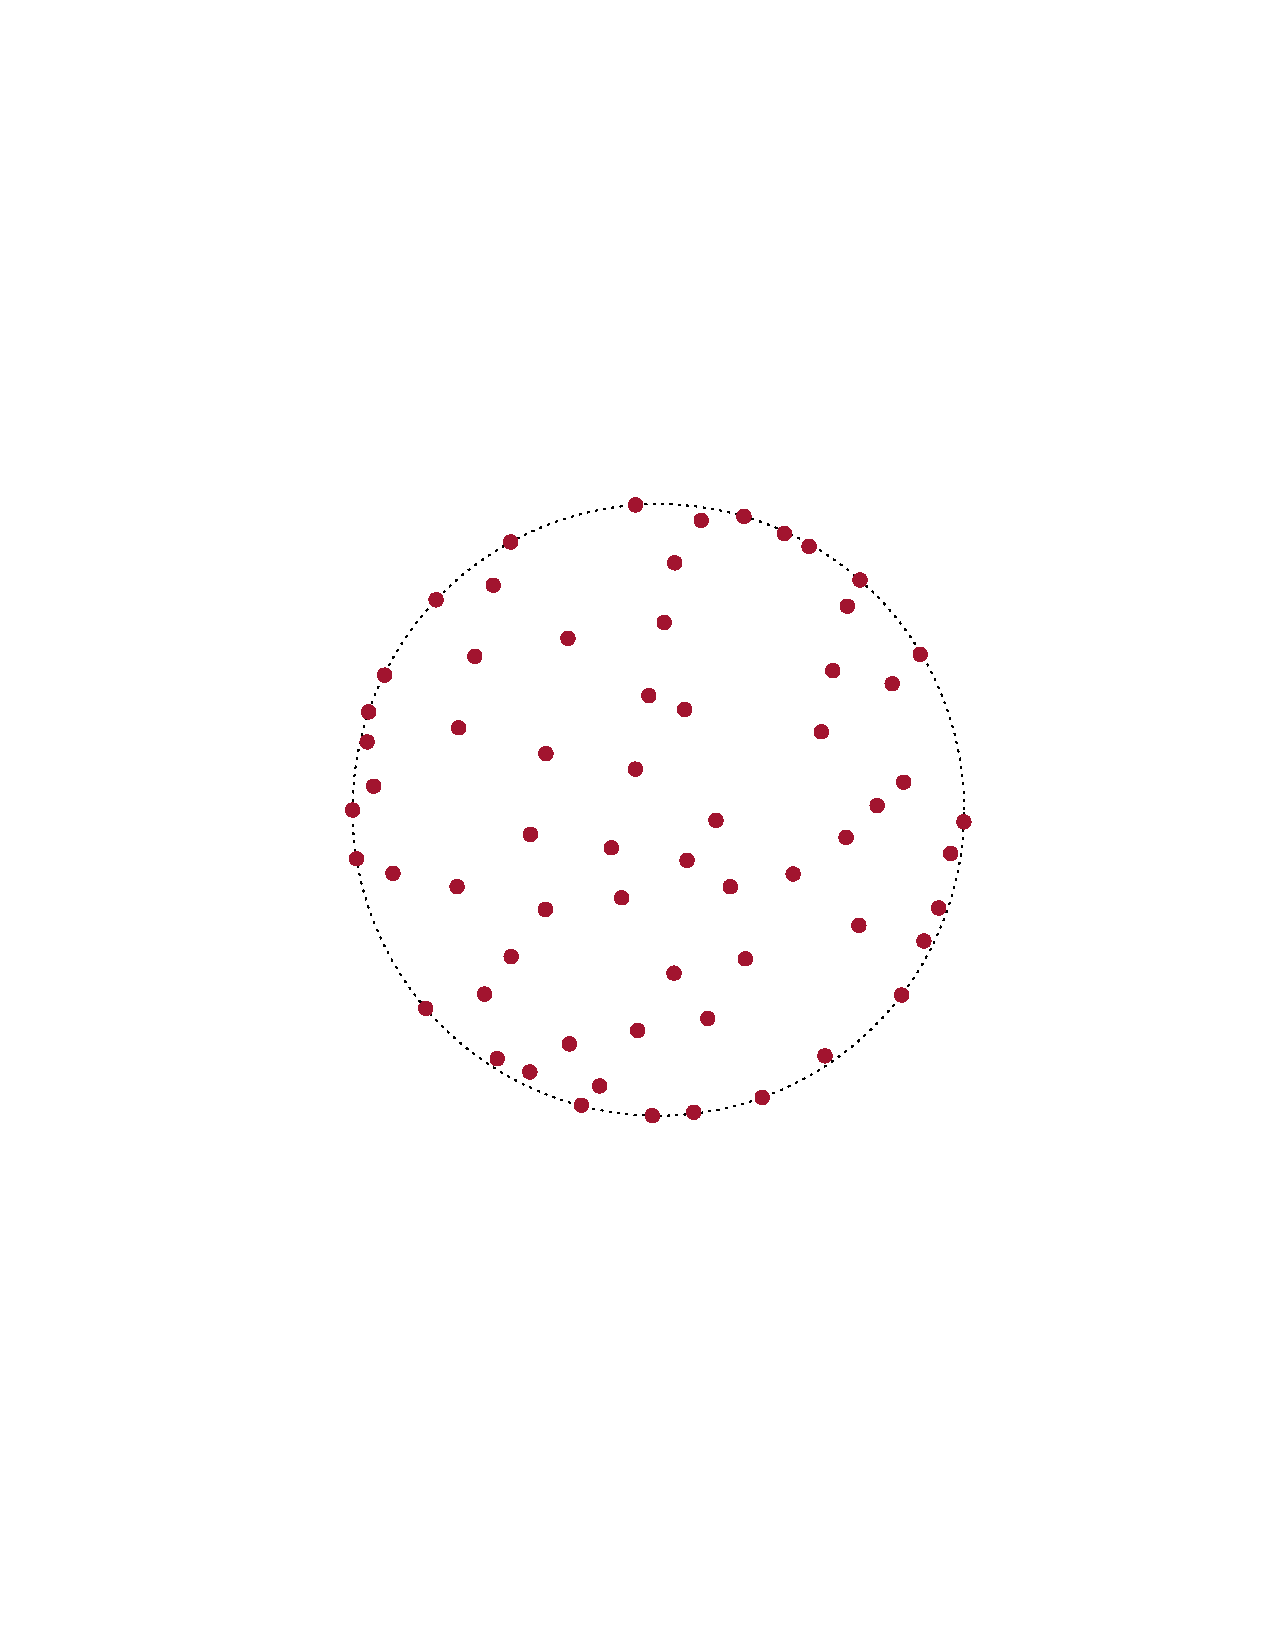
\includegraphics[clip, width=0.3\textwidth, scale=0.025, trim={3cm 8cm 3cm 8cm}]{figures/iea37-opt64-par1.pdf}
	}
	\subfigure[\textit{sub2}]{
		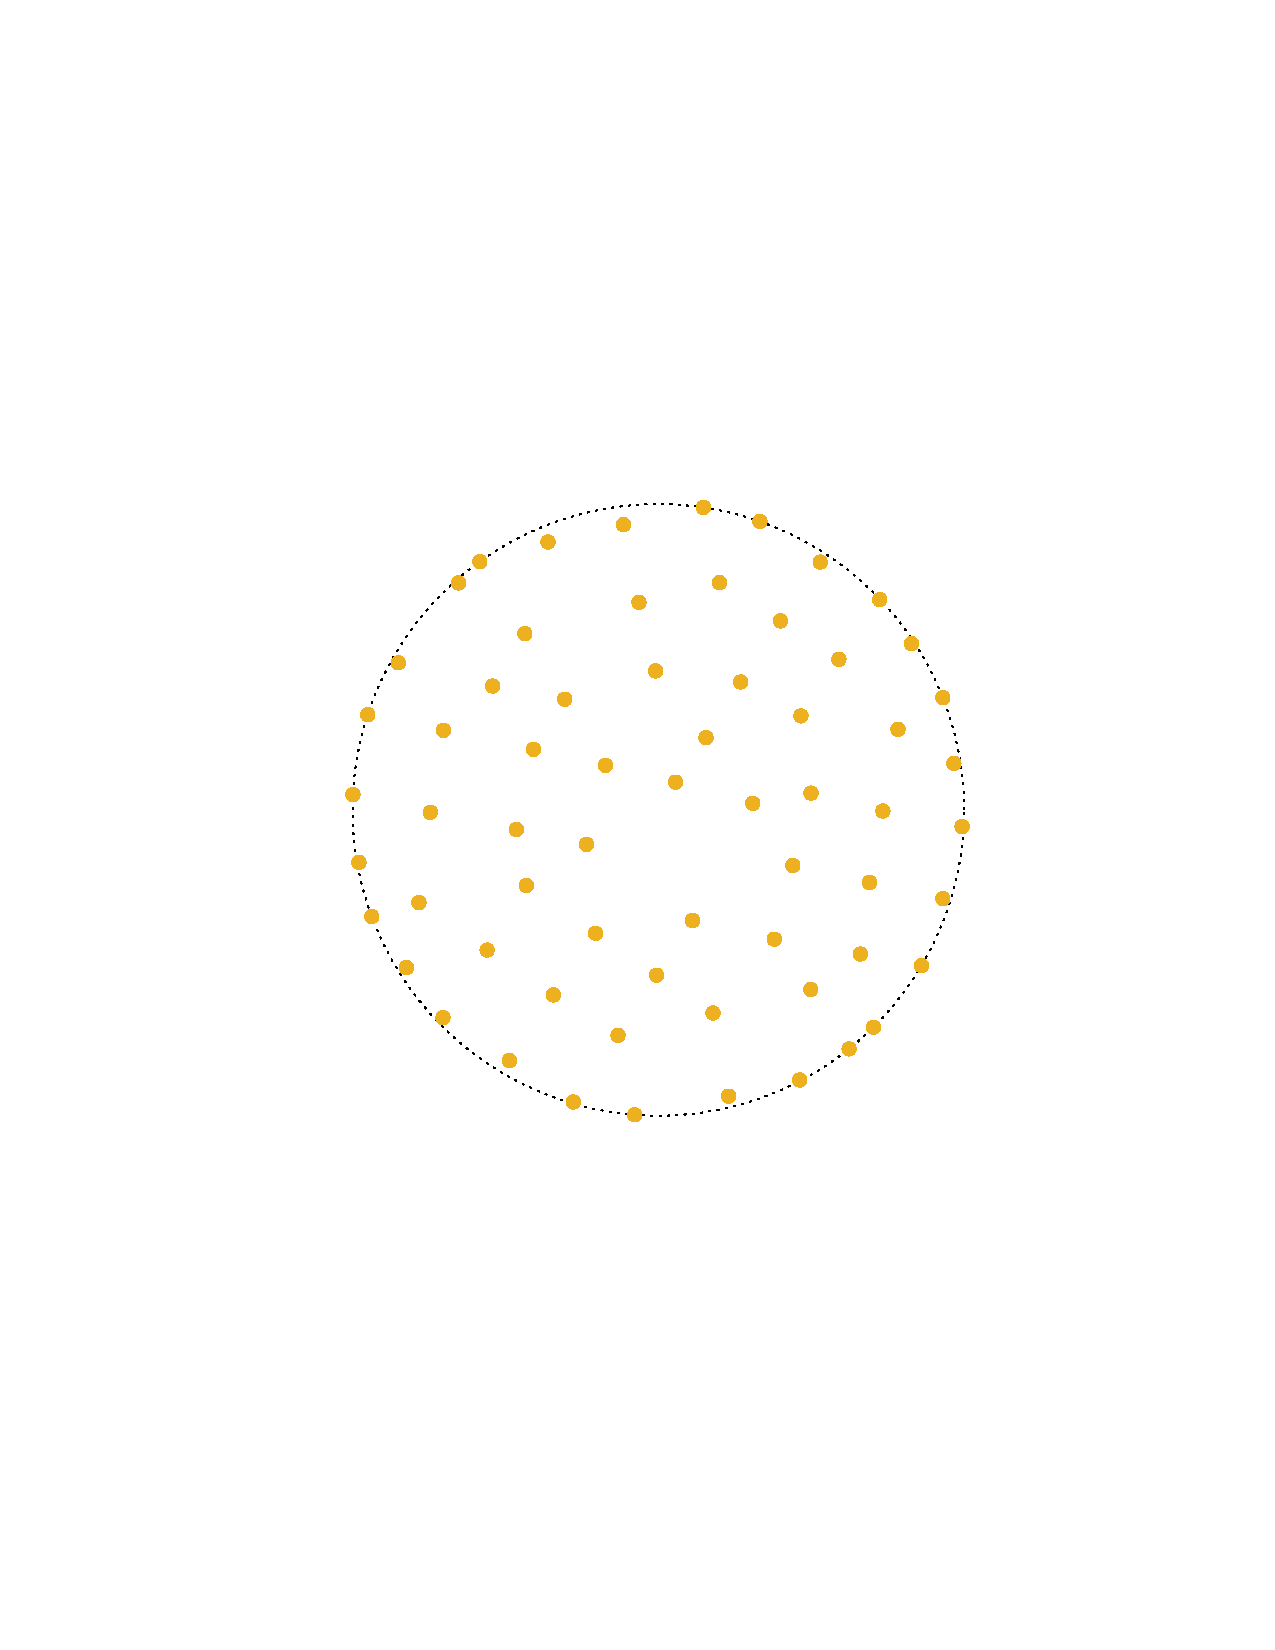
\includegraphics[clip, width=0.3\textwidth,scale=0.025, trim={3cm 8cm 3cm 8cm}]{figures/iea37-opt64-par2.pdf}
	}
	\subfigure[\textit{sub3}]{
		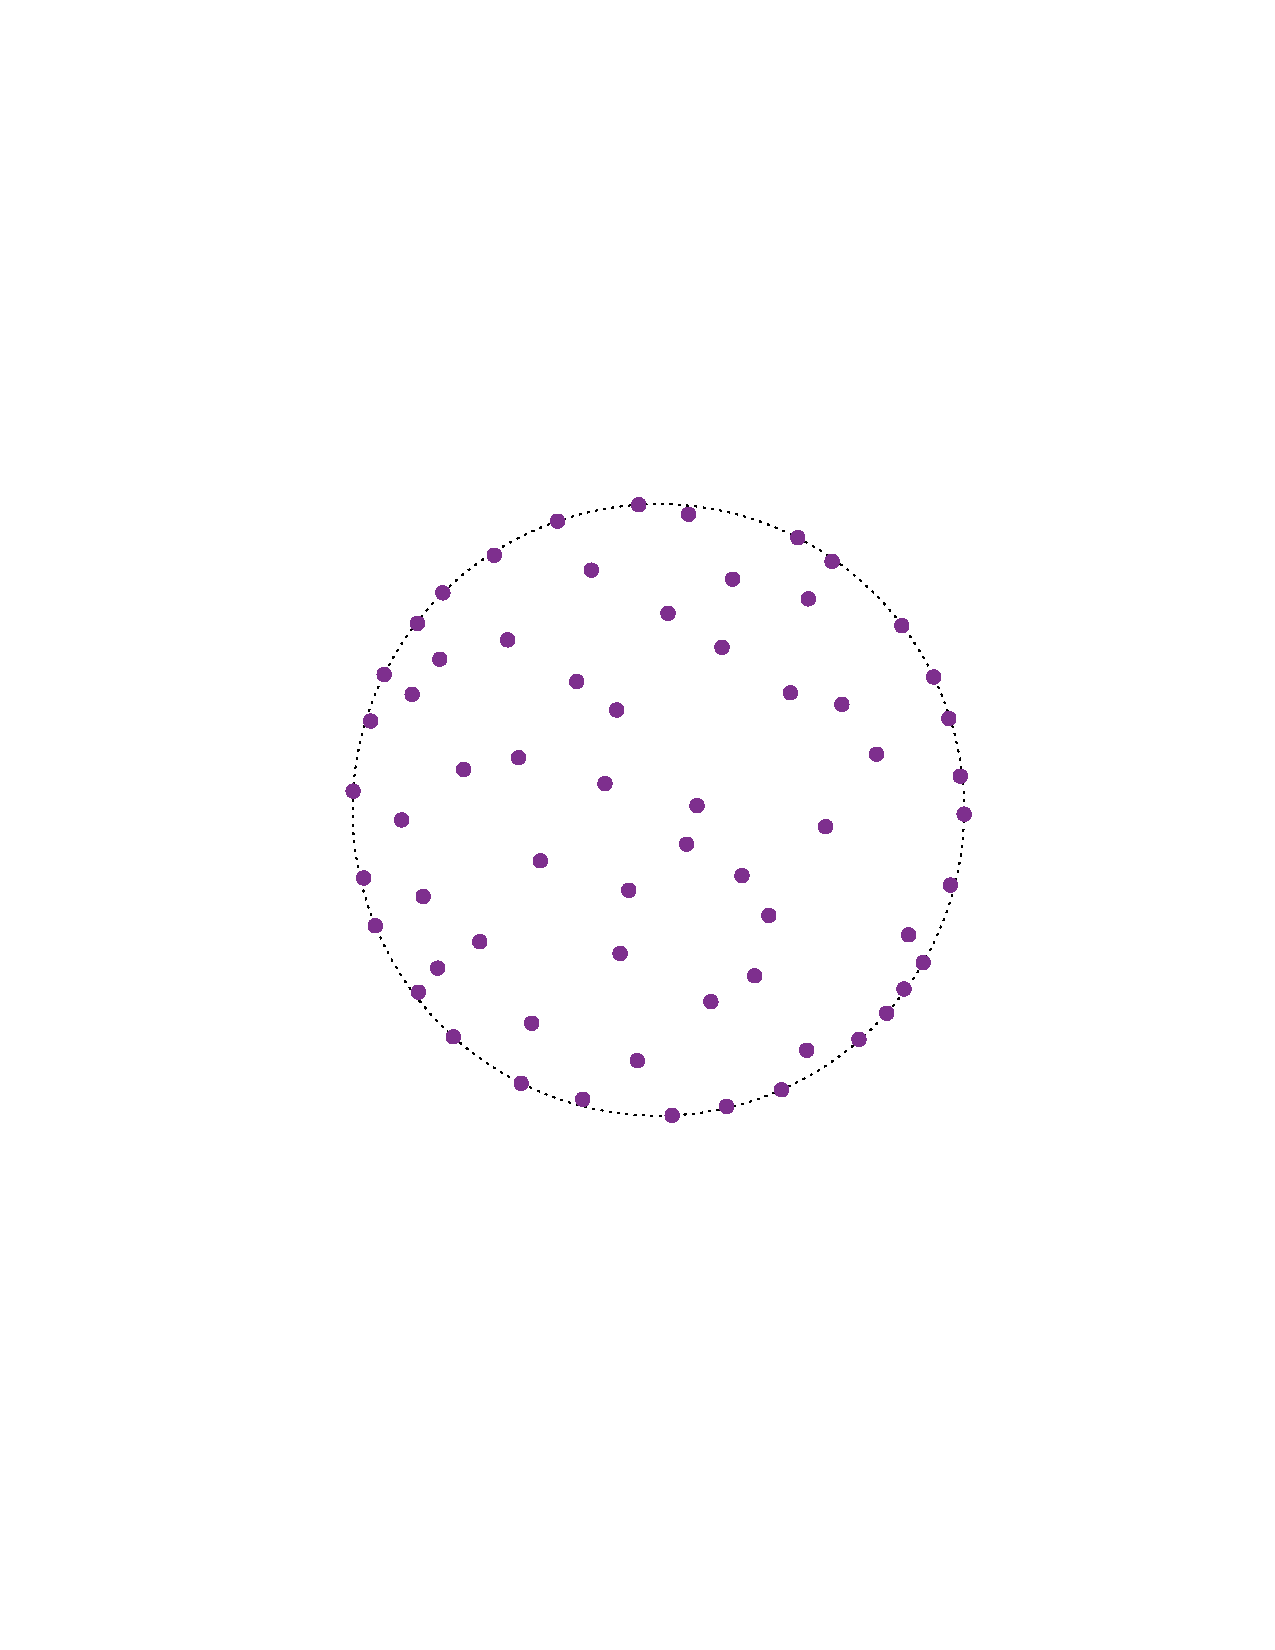
\includegraphics[clip, width=0.3\textwidth,scale=0.025, trim={3cm 8cm 3cm 8cm}]{figures/iea37-opt64-par3.pdf}
	}
	\subfigure[\textit{sub4}]{
		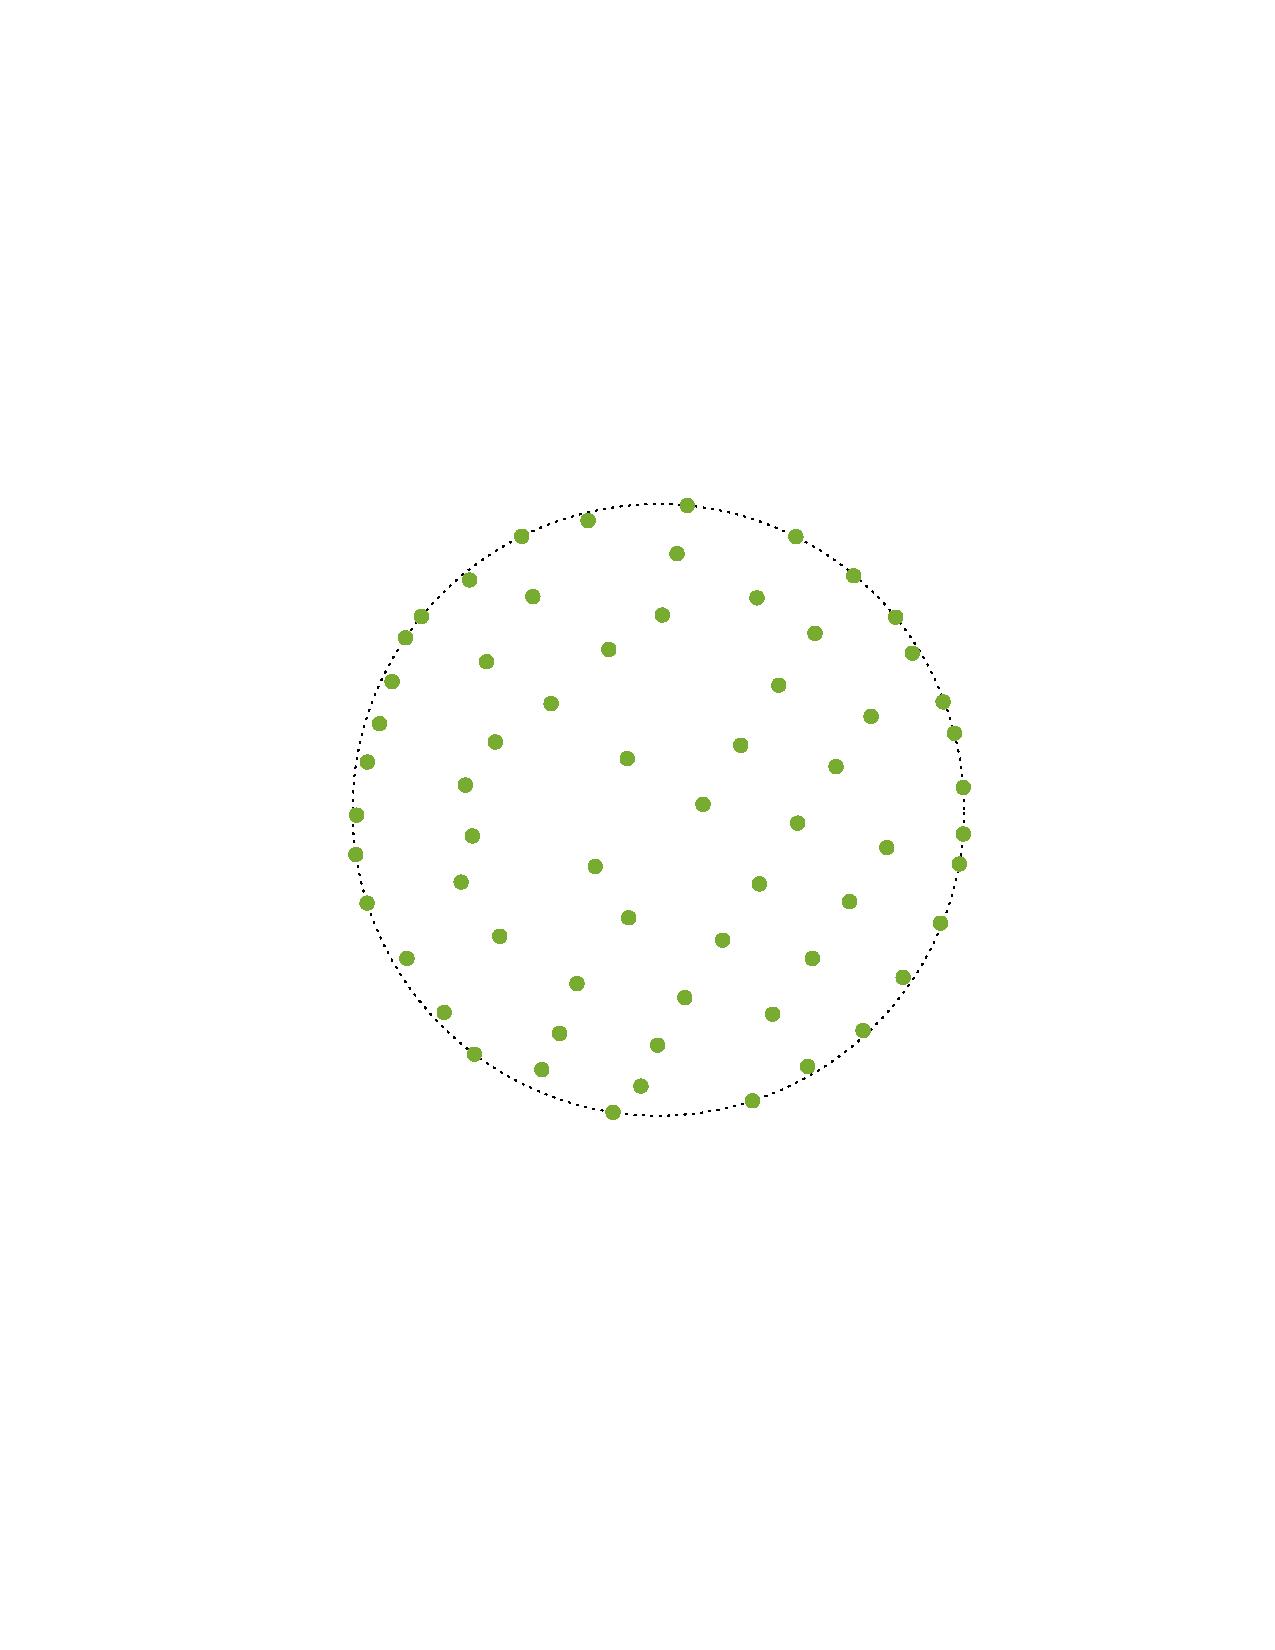
\includegraphics[clip, width=0.3\textwidth, scale=0.025, trim={3cm 8cm 3cm 8cm}]{figures/iea37-opt64-par4.pdf}
	}
	\subfigure[\textit{sub5}]{
		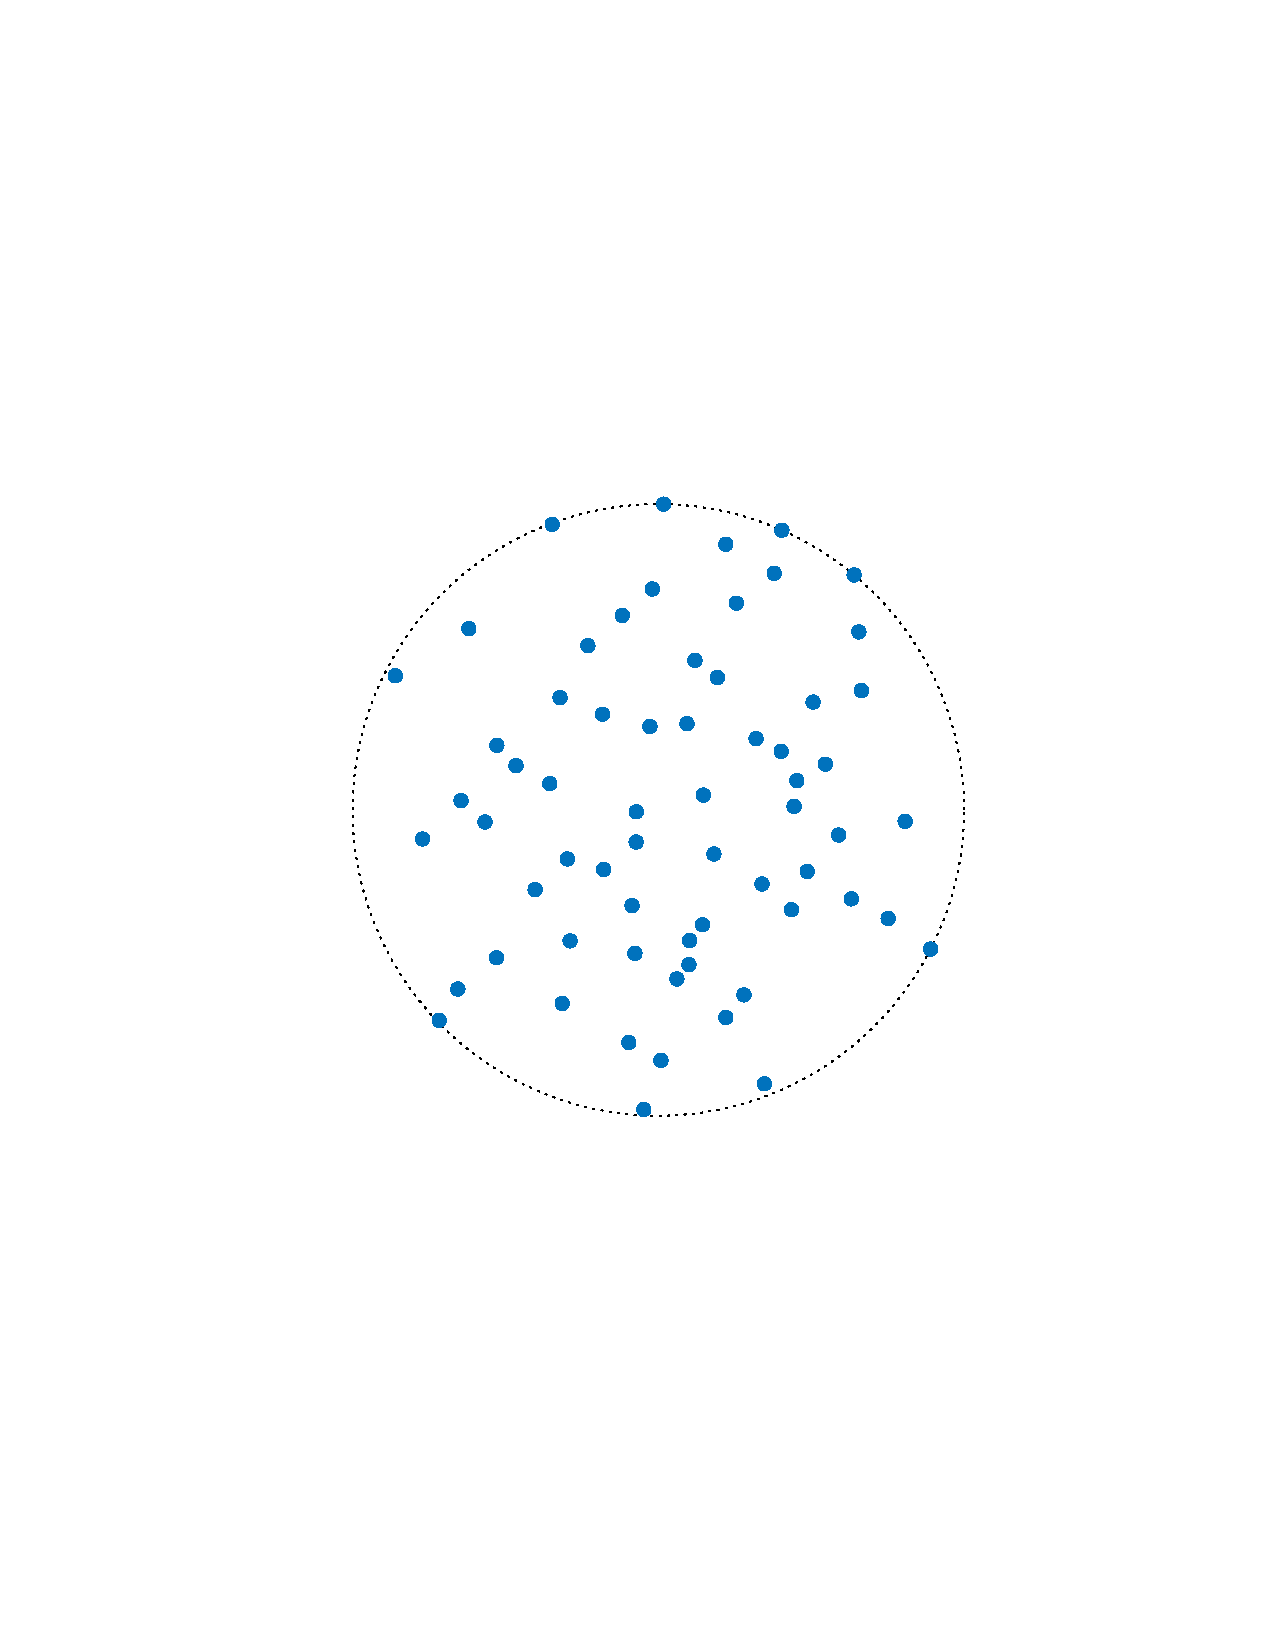
\includegraphics[clip, width=0.3\textwidth, scale=0.025, trim={3cm 8cm 3cm 8cm}]{figures/iea37-opt64-par5.pdf}
	}
	\subfigure[\textit{sub6}]{
		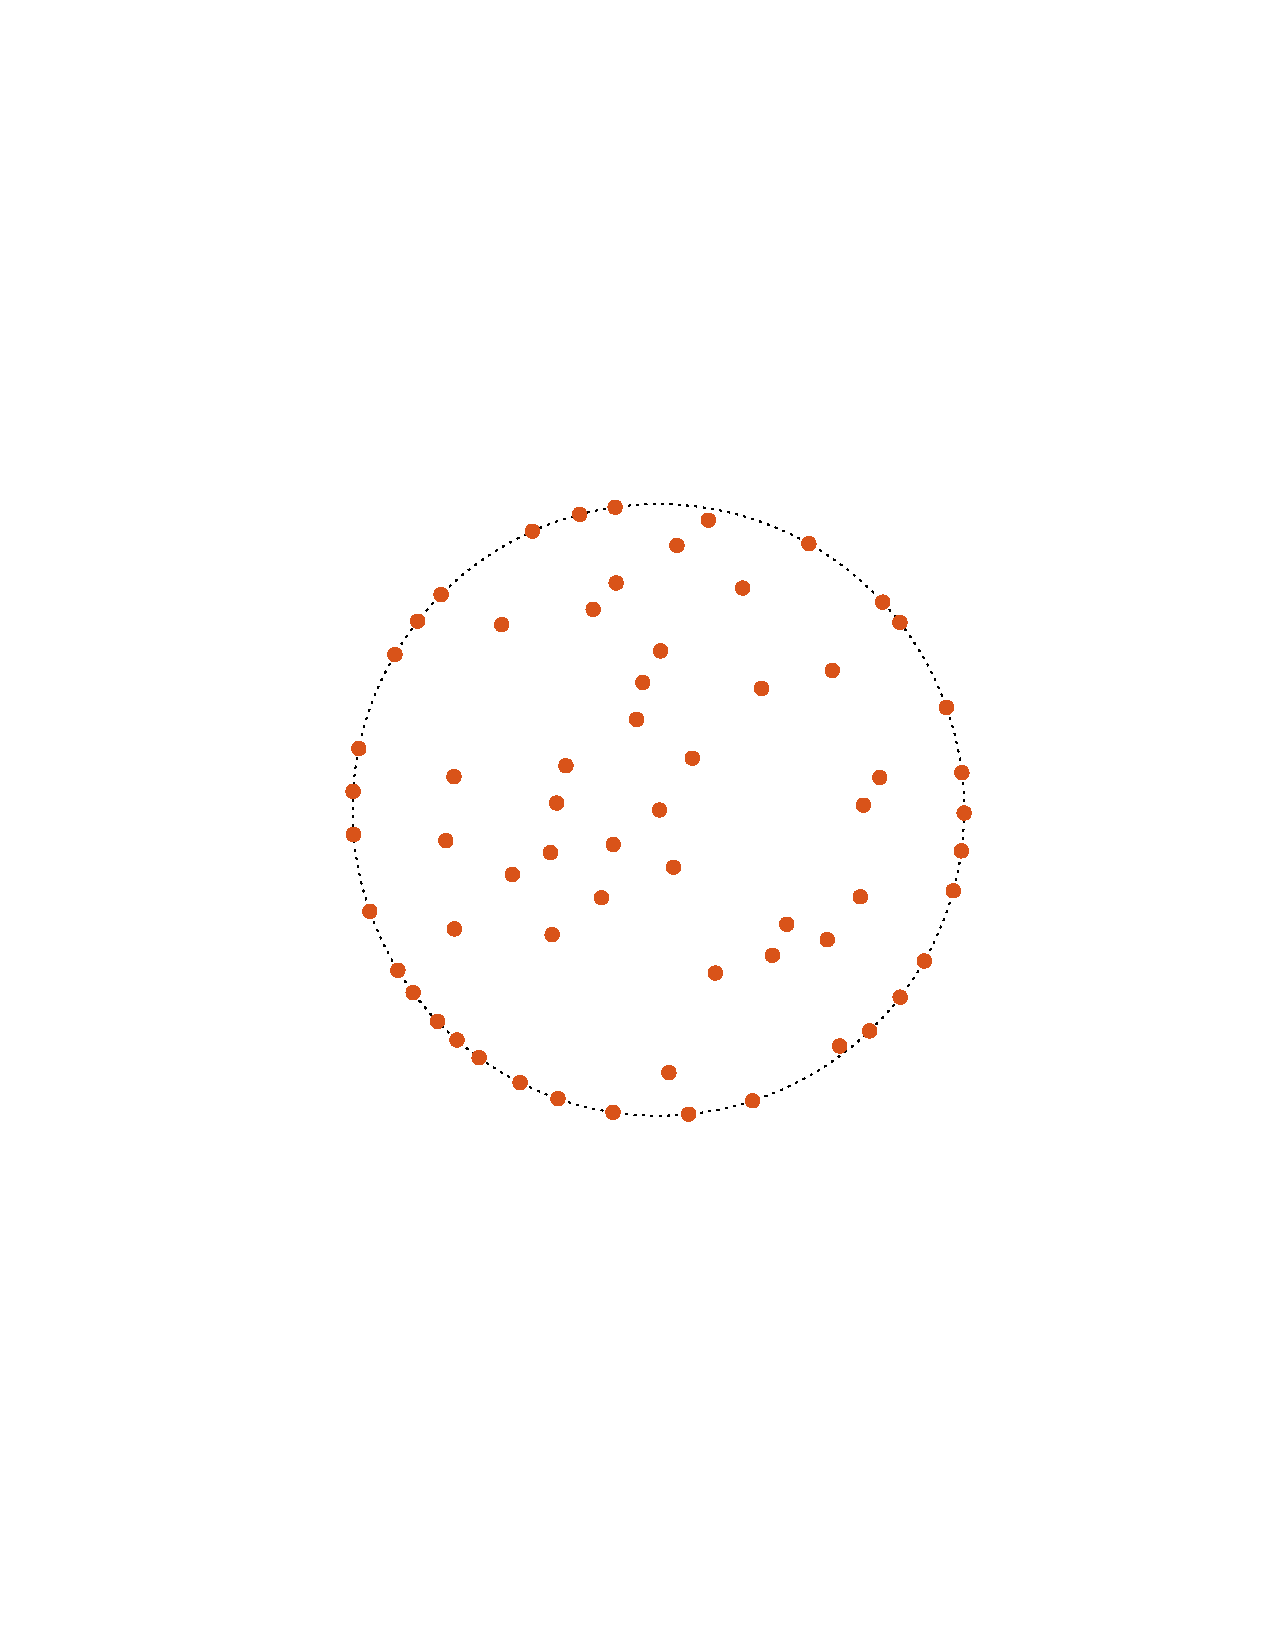
\includegraphics[clip, width=0.3\textwidth, scale=0.025, trim={3cm 8cm 3cm 8cm}]{figures/iea37-opt64-par6.pdf}
	}
	\subfigure[\textit{sub7}]{
		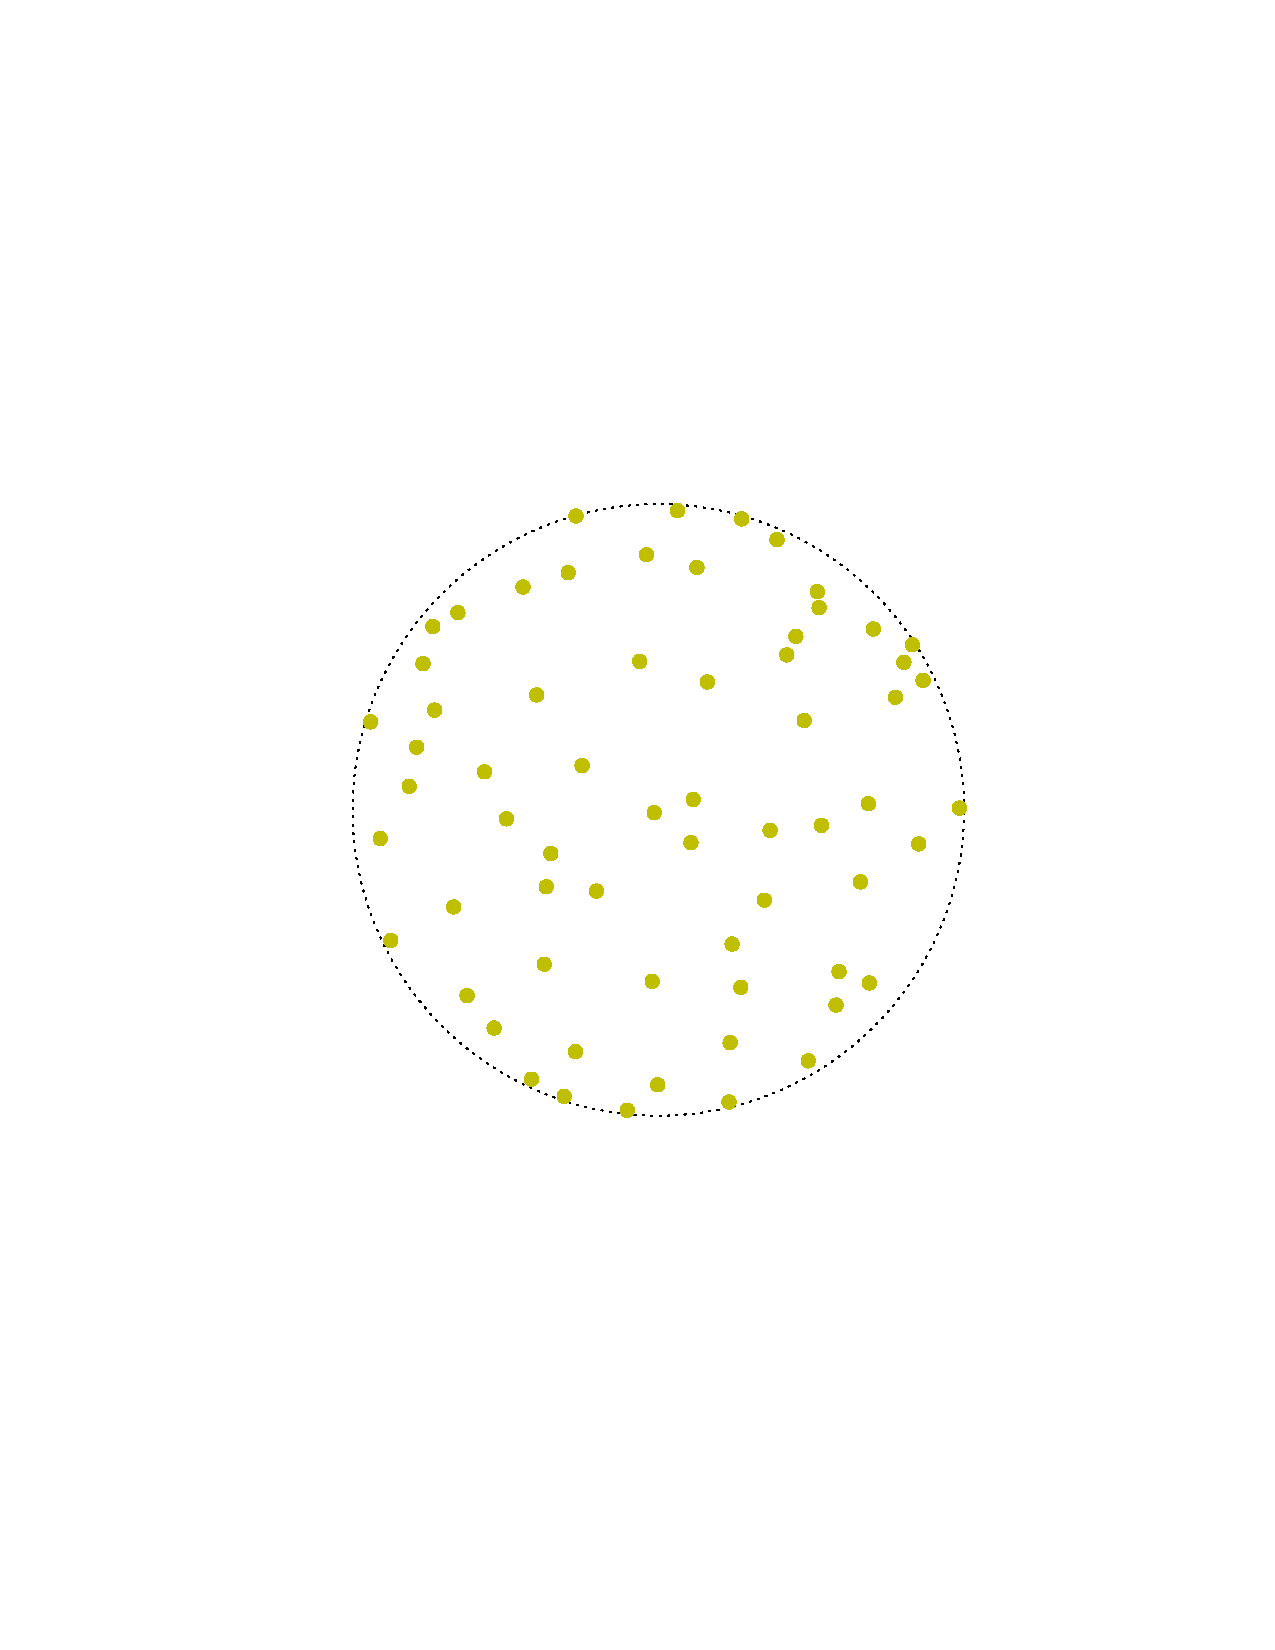
\includegraphics[clip, width=0.3\textwidth,scale=0.025, trim={3cm 8cm 3cm 8cm}]{figures/iea37-opt64-par7.pdf}
	}
	\subfigure[\textit{sub8}]{
		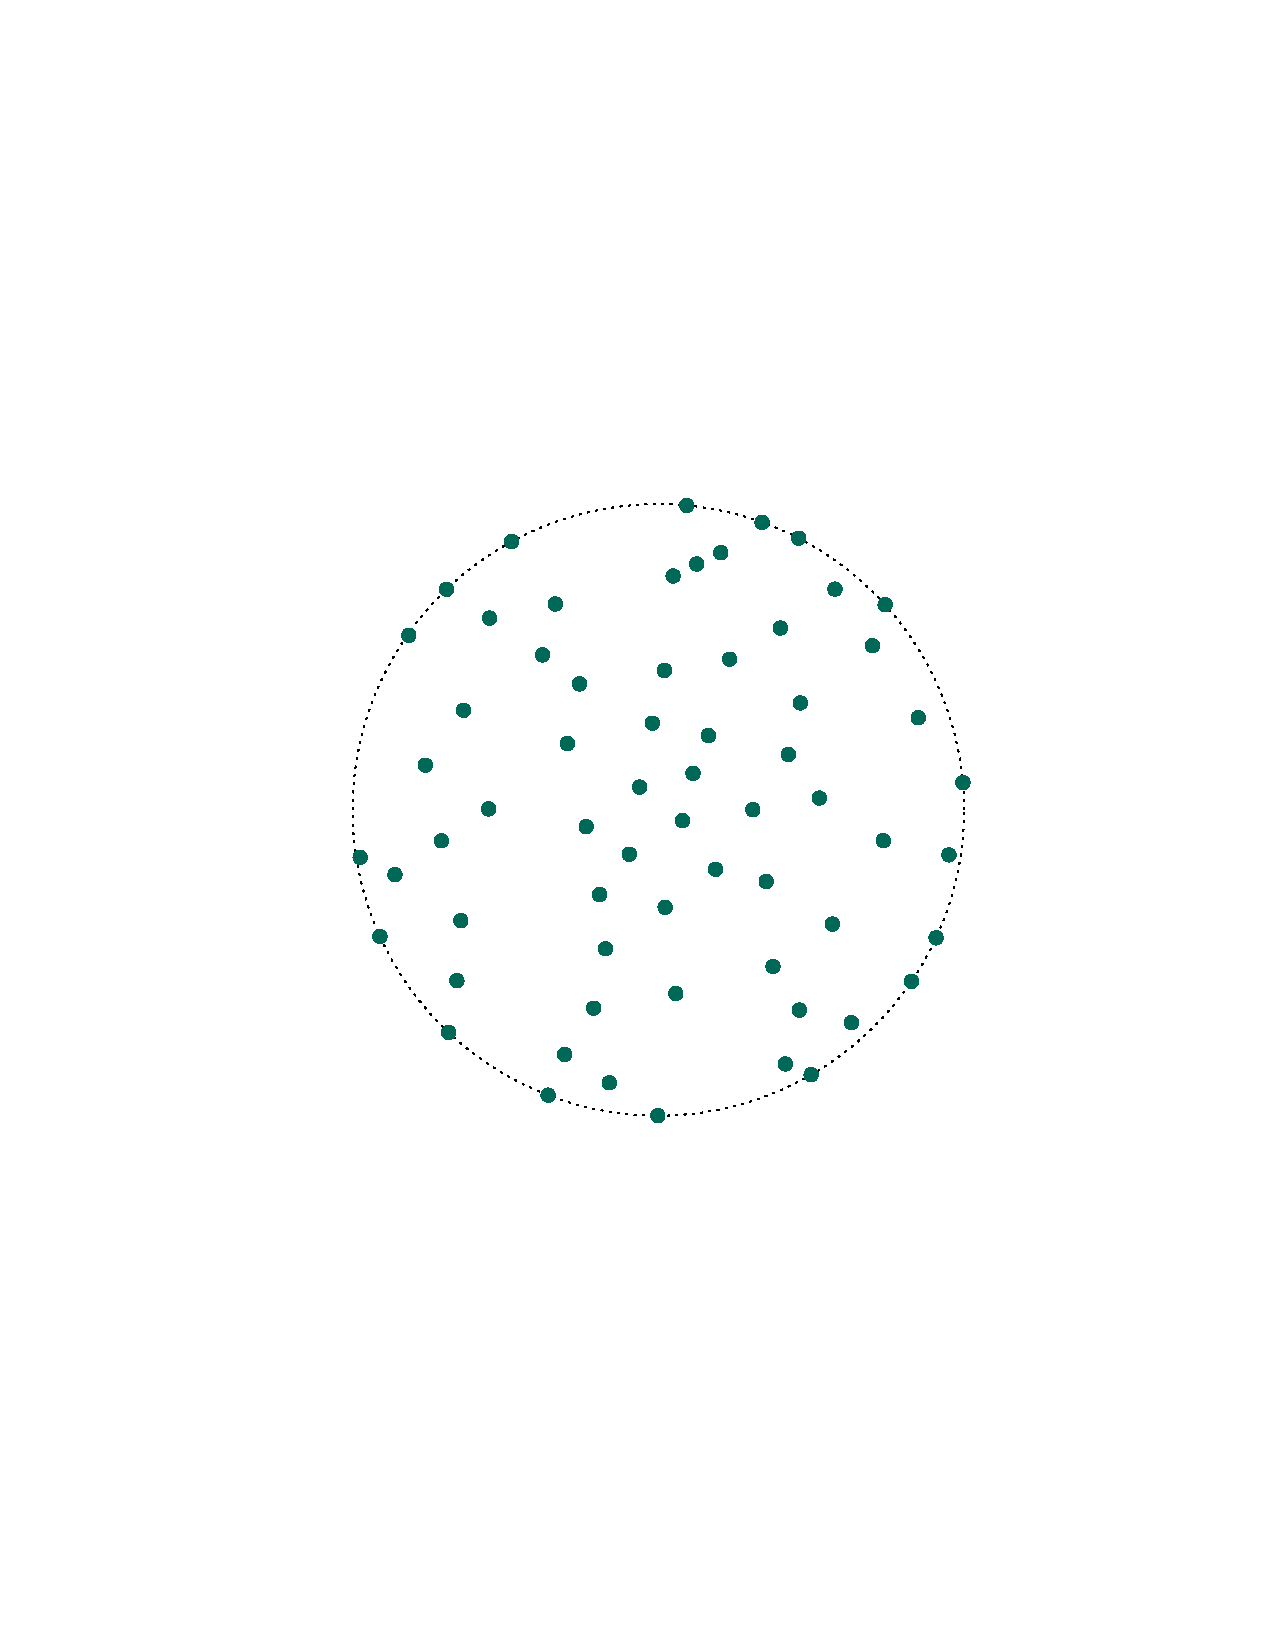
\includegraphics[clip, width=0.3\textwidth,scale=0.025, trim={3cm 8cm 3cm 8cm}]{figures/iea37-opt64-par8.pdf}
	}
	\subfigure[\textit{sub9}]{
		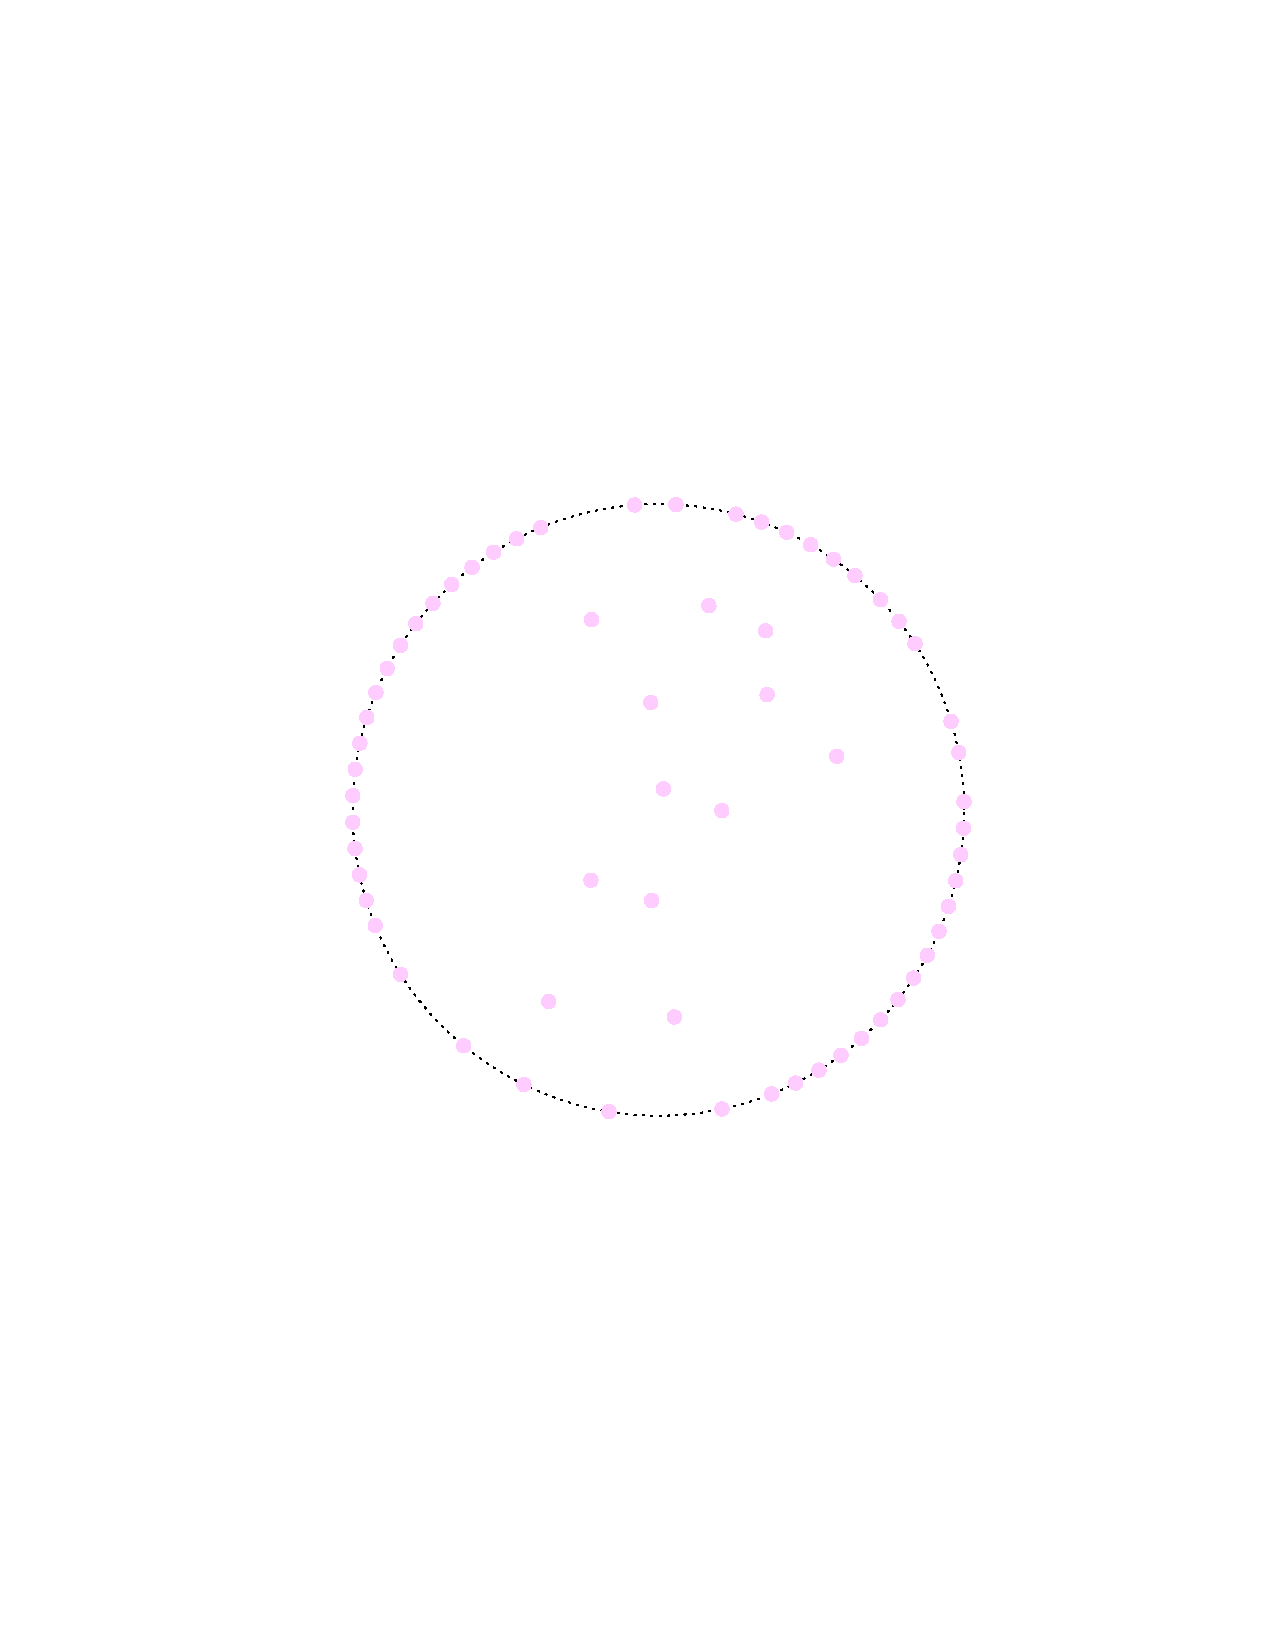
\includegraphics[clip, width=0.3\textwidth, scale=0.025, trim={3cm 8cm 3cm 8cm}]{figures/iea37-opt64-par9.pdf}
	}
	\subfigure[\textit{sub10}]{
		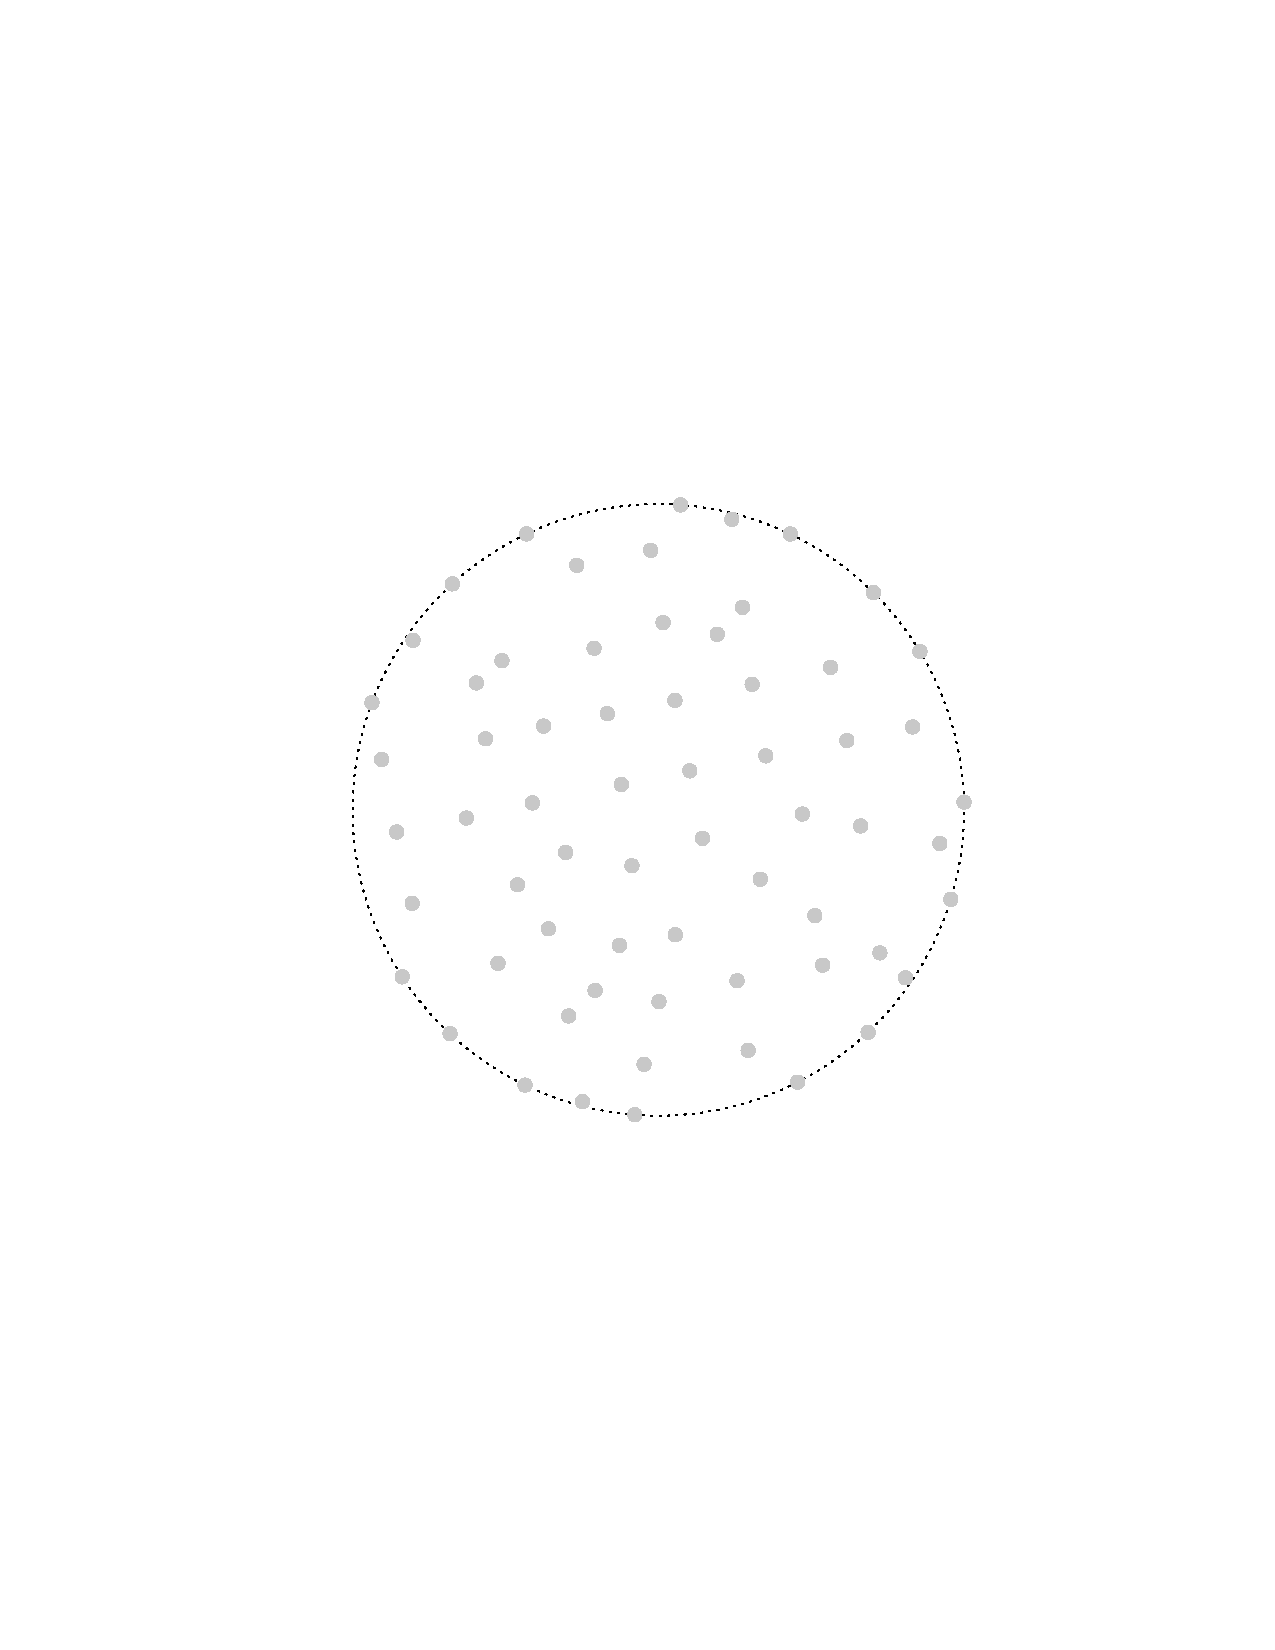
\includegraphics[clip, width=0.3\textwidth, scale=0.025, trim={3cm 8cm 3cm 8cm}]{figures/iea37-opt64-par10.pdf}
	}
	\caption{Case study 1: optimized wind farm layouts with 64 wind turbines.}
	
	\label{fig:64turbs}
\end{figure}

\begin{figure}[htbp!]
	\centering
	\subfigure[\textit{sub1}]{
		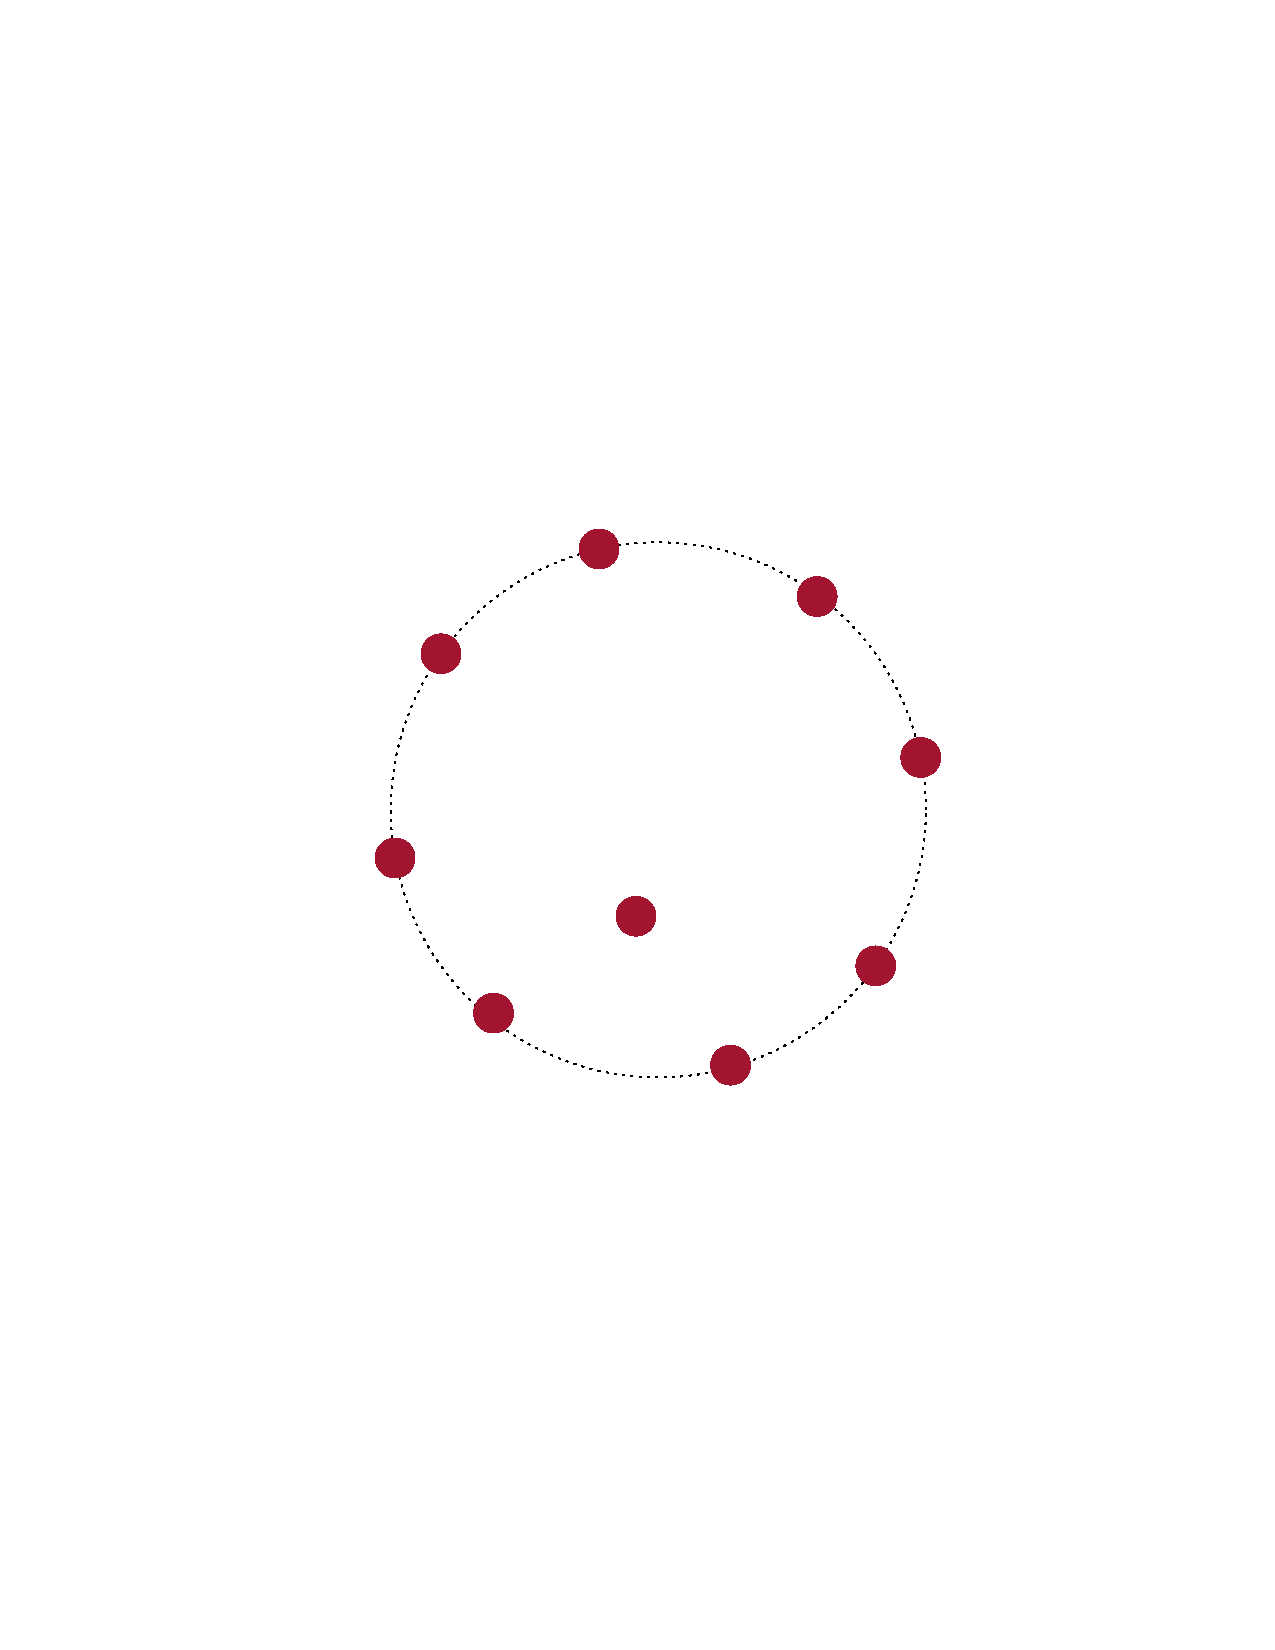
\includegraphics[clip, width=0.45\textwidth, scale=0.025, trim={3cm 8cm 3cm 8cm}]{figures/iea37-opt9-par1.pdf}
	}
	\subfigure[\textit{sub2}]{
		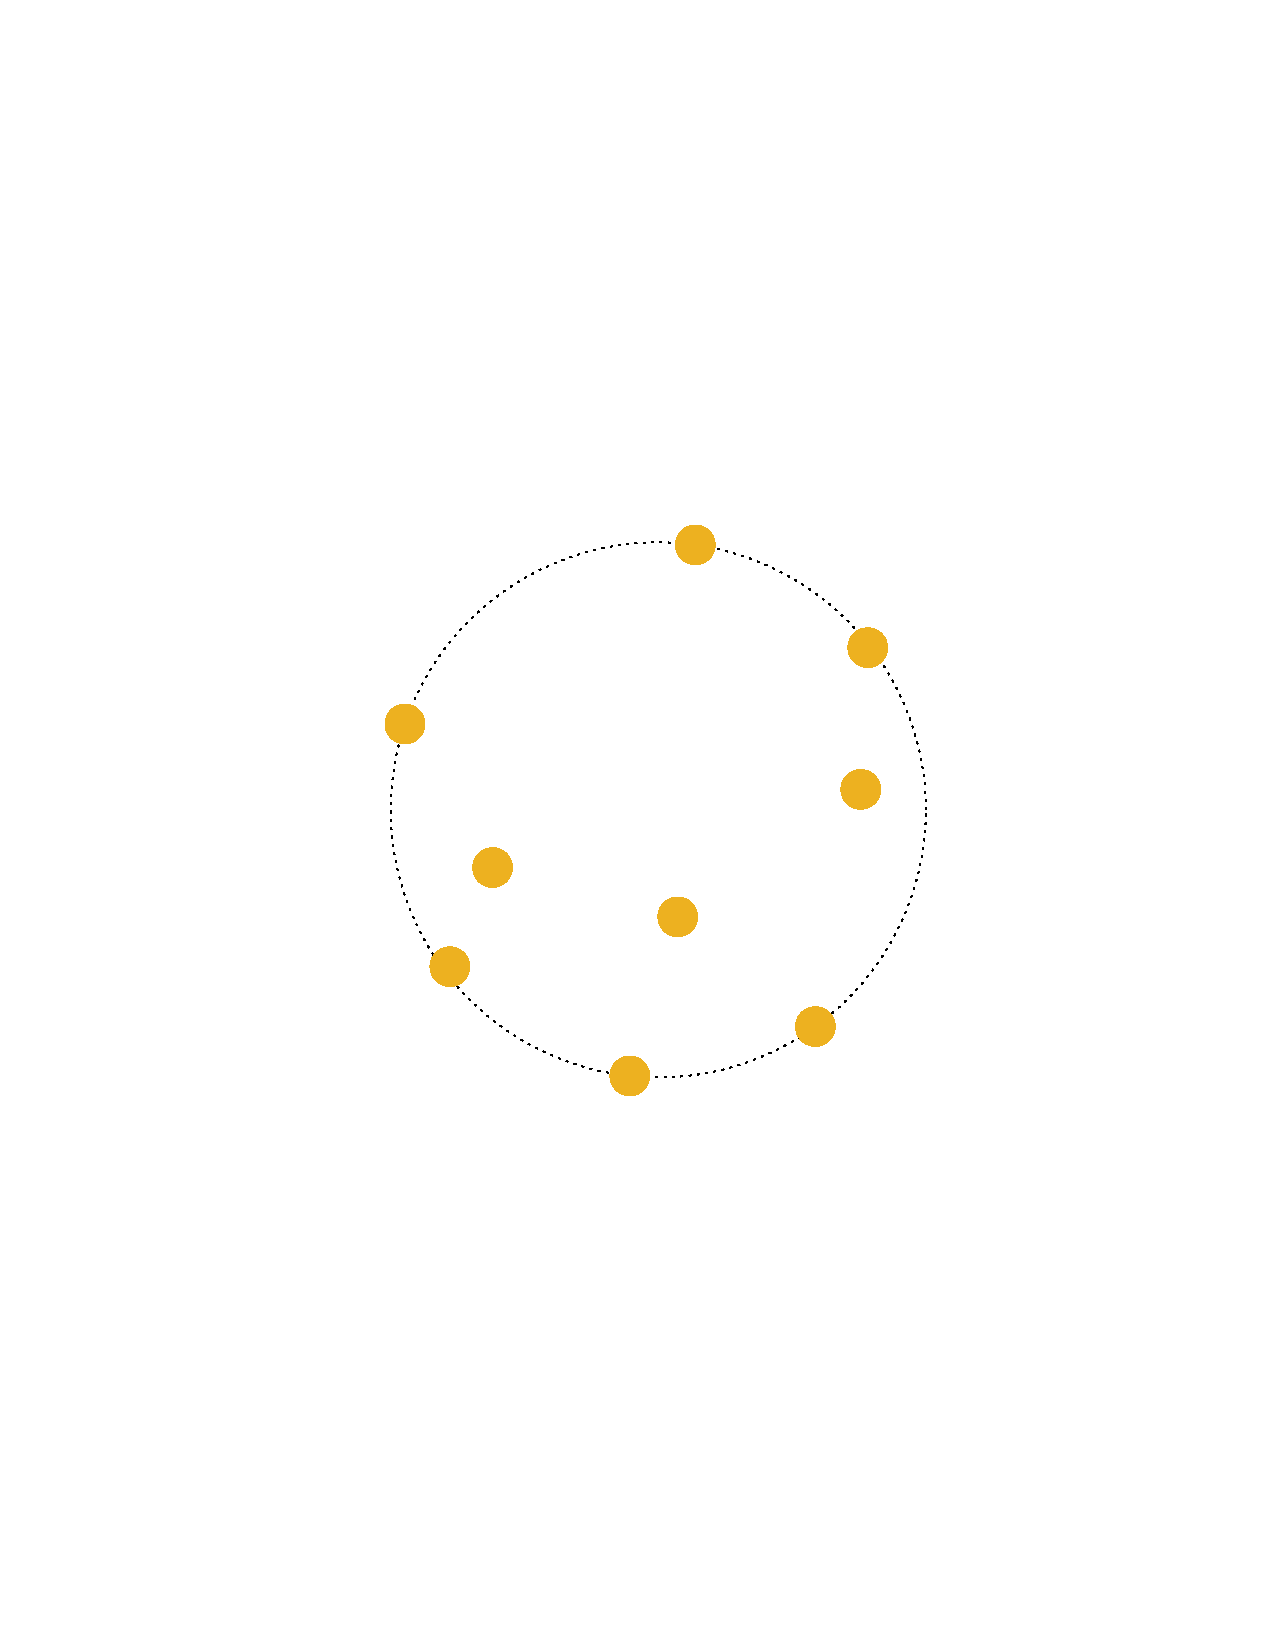
\includegraphics[clip, width=0.45\textwidth,scale=0.025, trim={3cm 8cm 3cm 8cm}]{figures/iea37-opt9-par2.pdf}
	}
	\subfigure[\textit{sub3}]{
		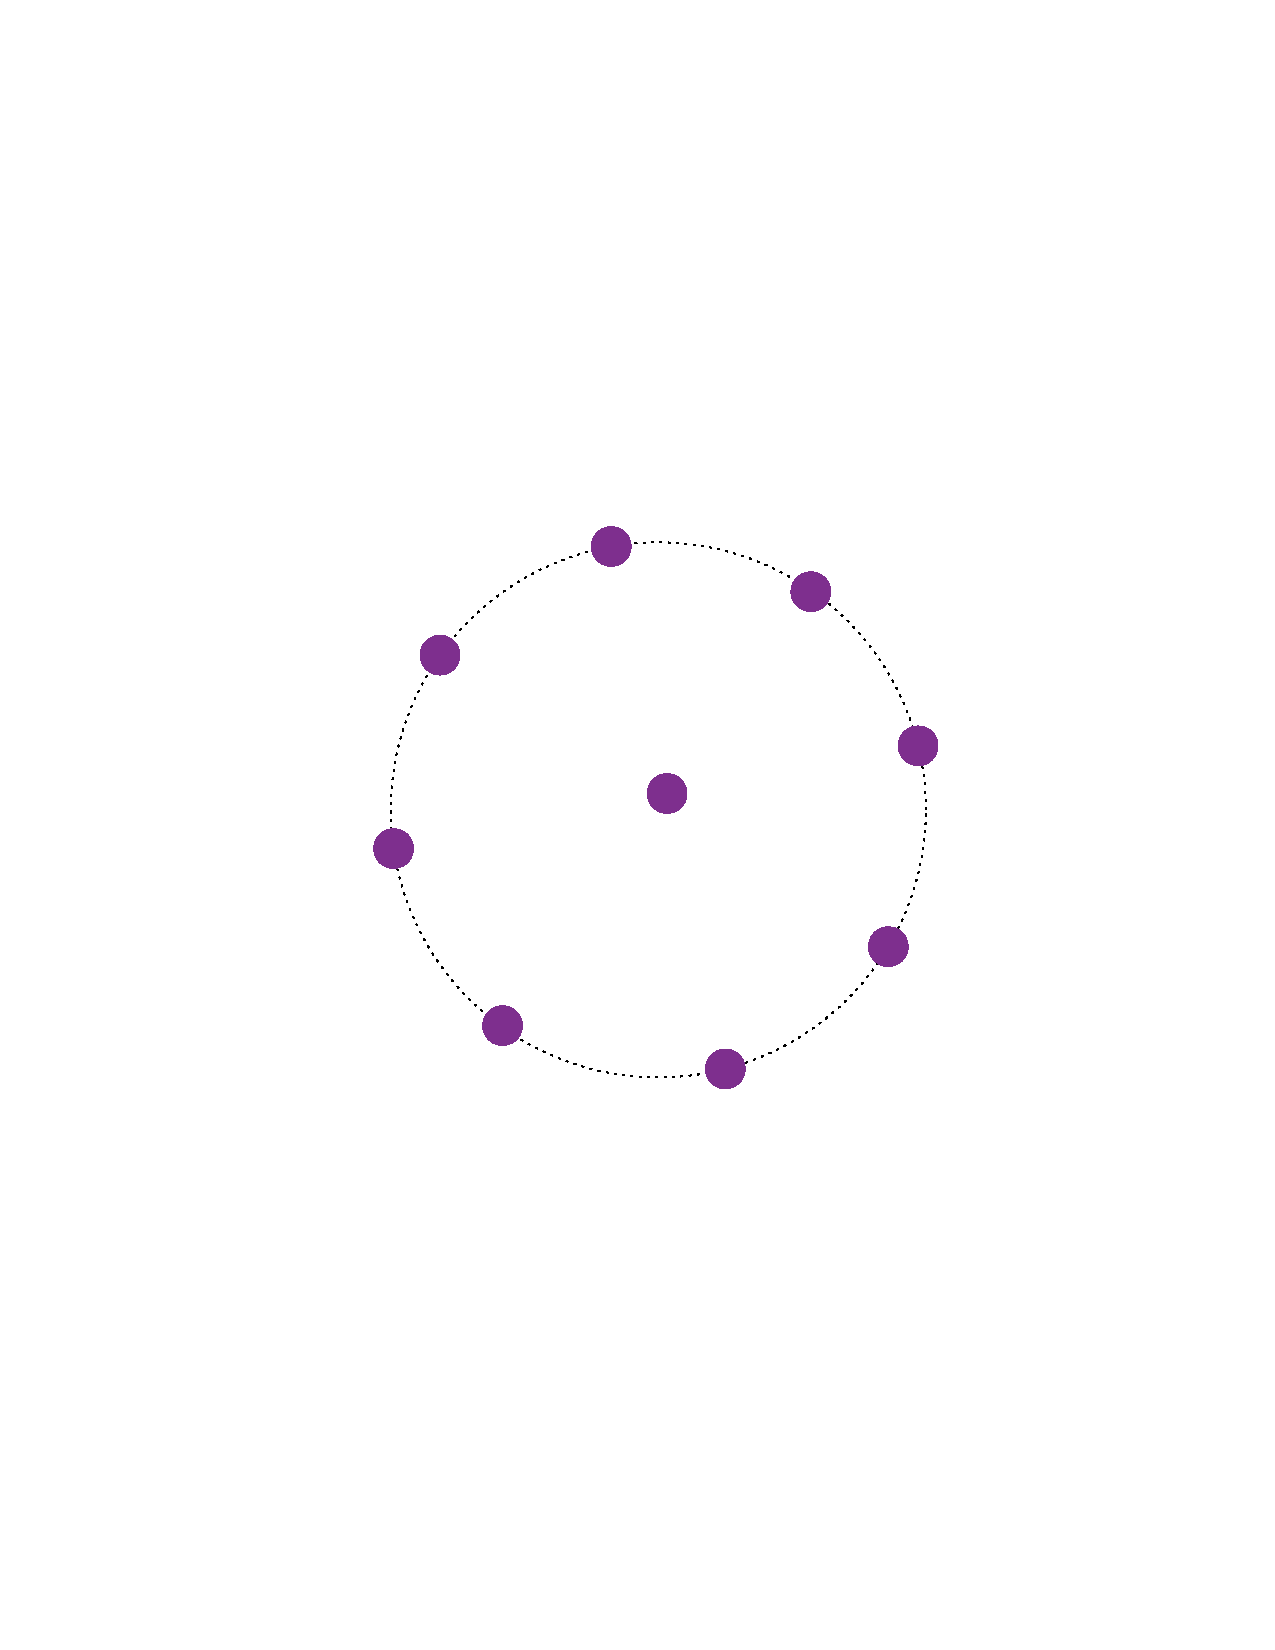
\includegraphics[clip, width=0.45\textwidth,scale=0.025, trim={3cm 8cm 3cm 8cm}]{figures/iea37-opt9-par3.pdf}
	}
	\subfigure[\textit{sub4}]{
		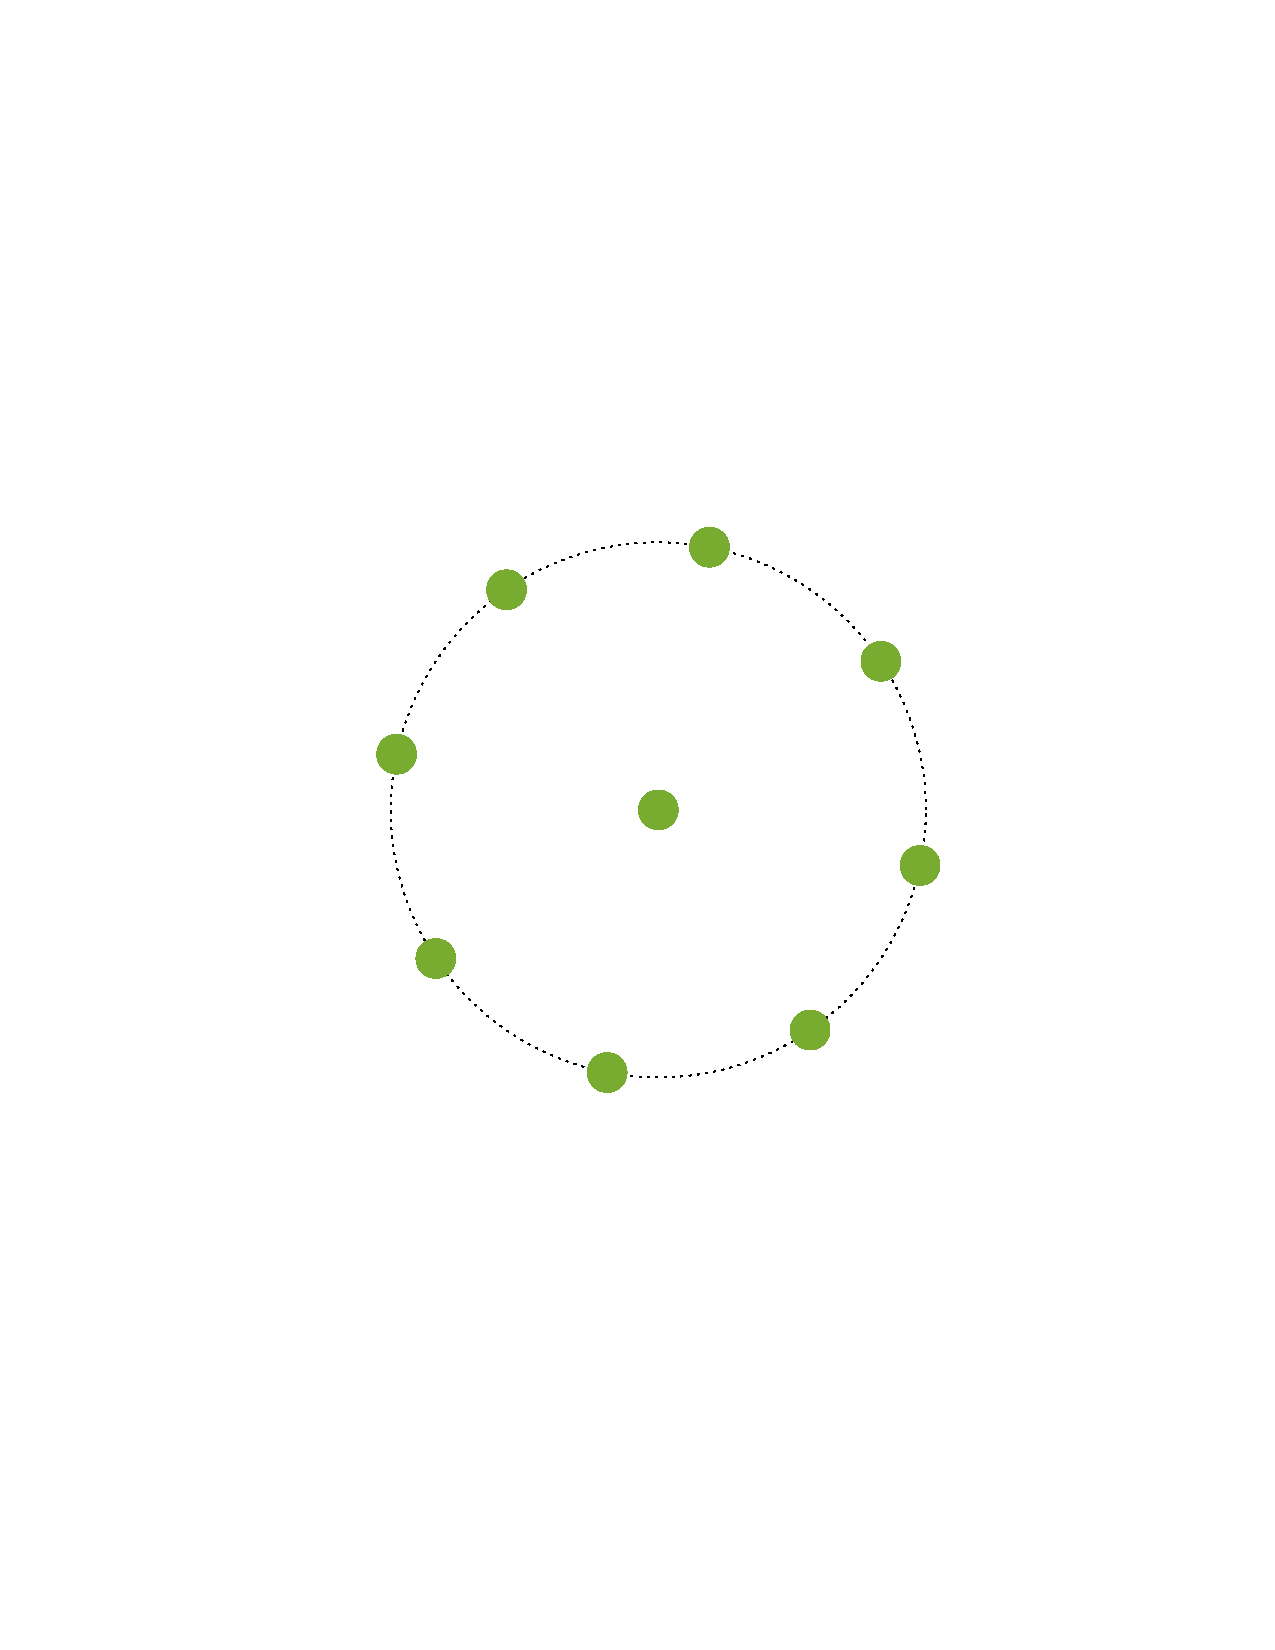
\includegraphics[clip, width=0.45\textwidth, scale=0.025, trim={3cm 8cm 3cm 8cm}]{figures/iea37-opt9-par4.pdf}
	}
	\subfigure[\textit{sub5}]{
		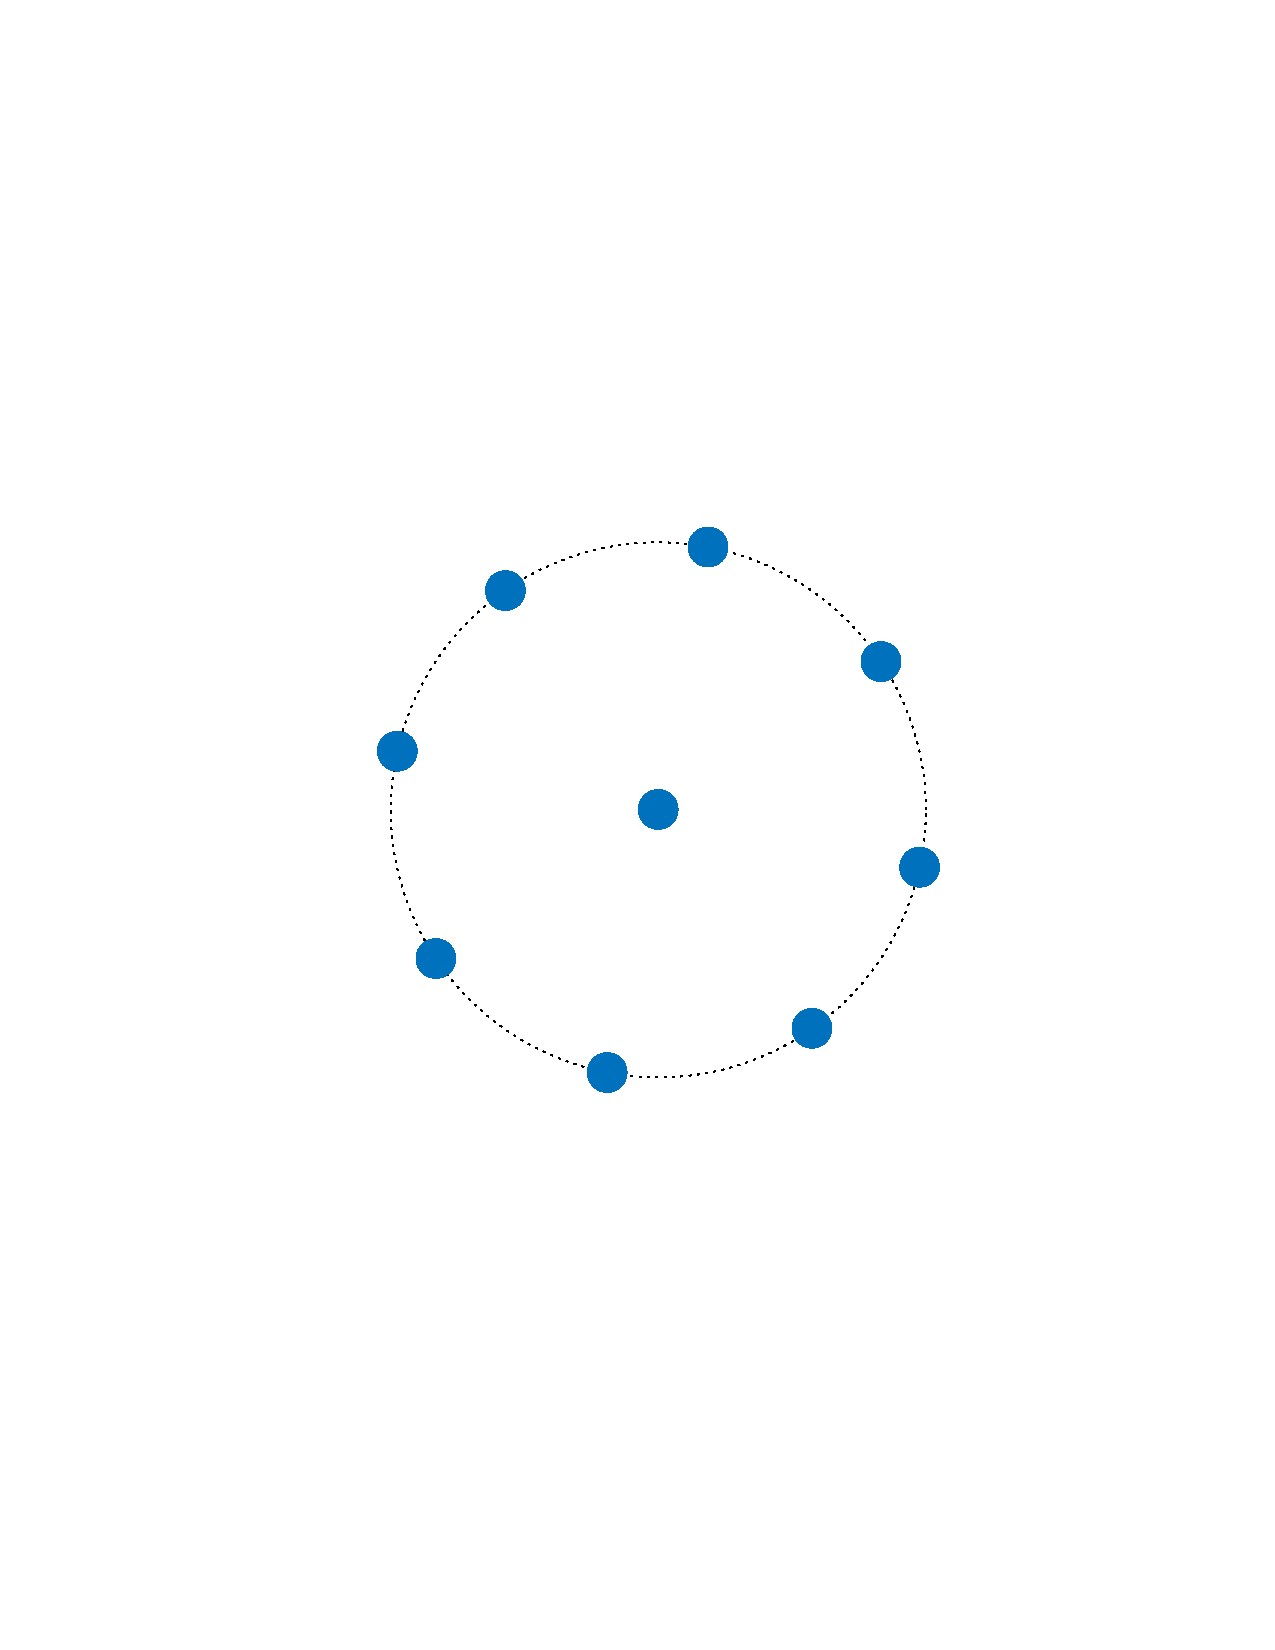
\includegraphics[clip, width=0.45\textwidth, scale=0.025, trim={3cm 8cm 3cm 8cm}]{figures/iea37-opt9-par5.pdf}
	}
	\caption{Case study 2: optimized wind farm layouts with 9 wind turbines.}
	
	\label{fig:9turbs}
\end{figure}

% 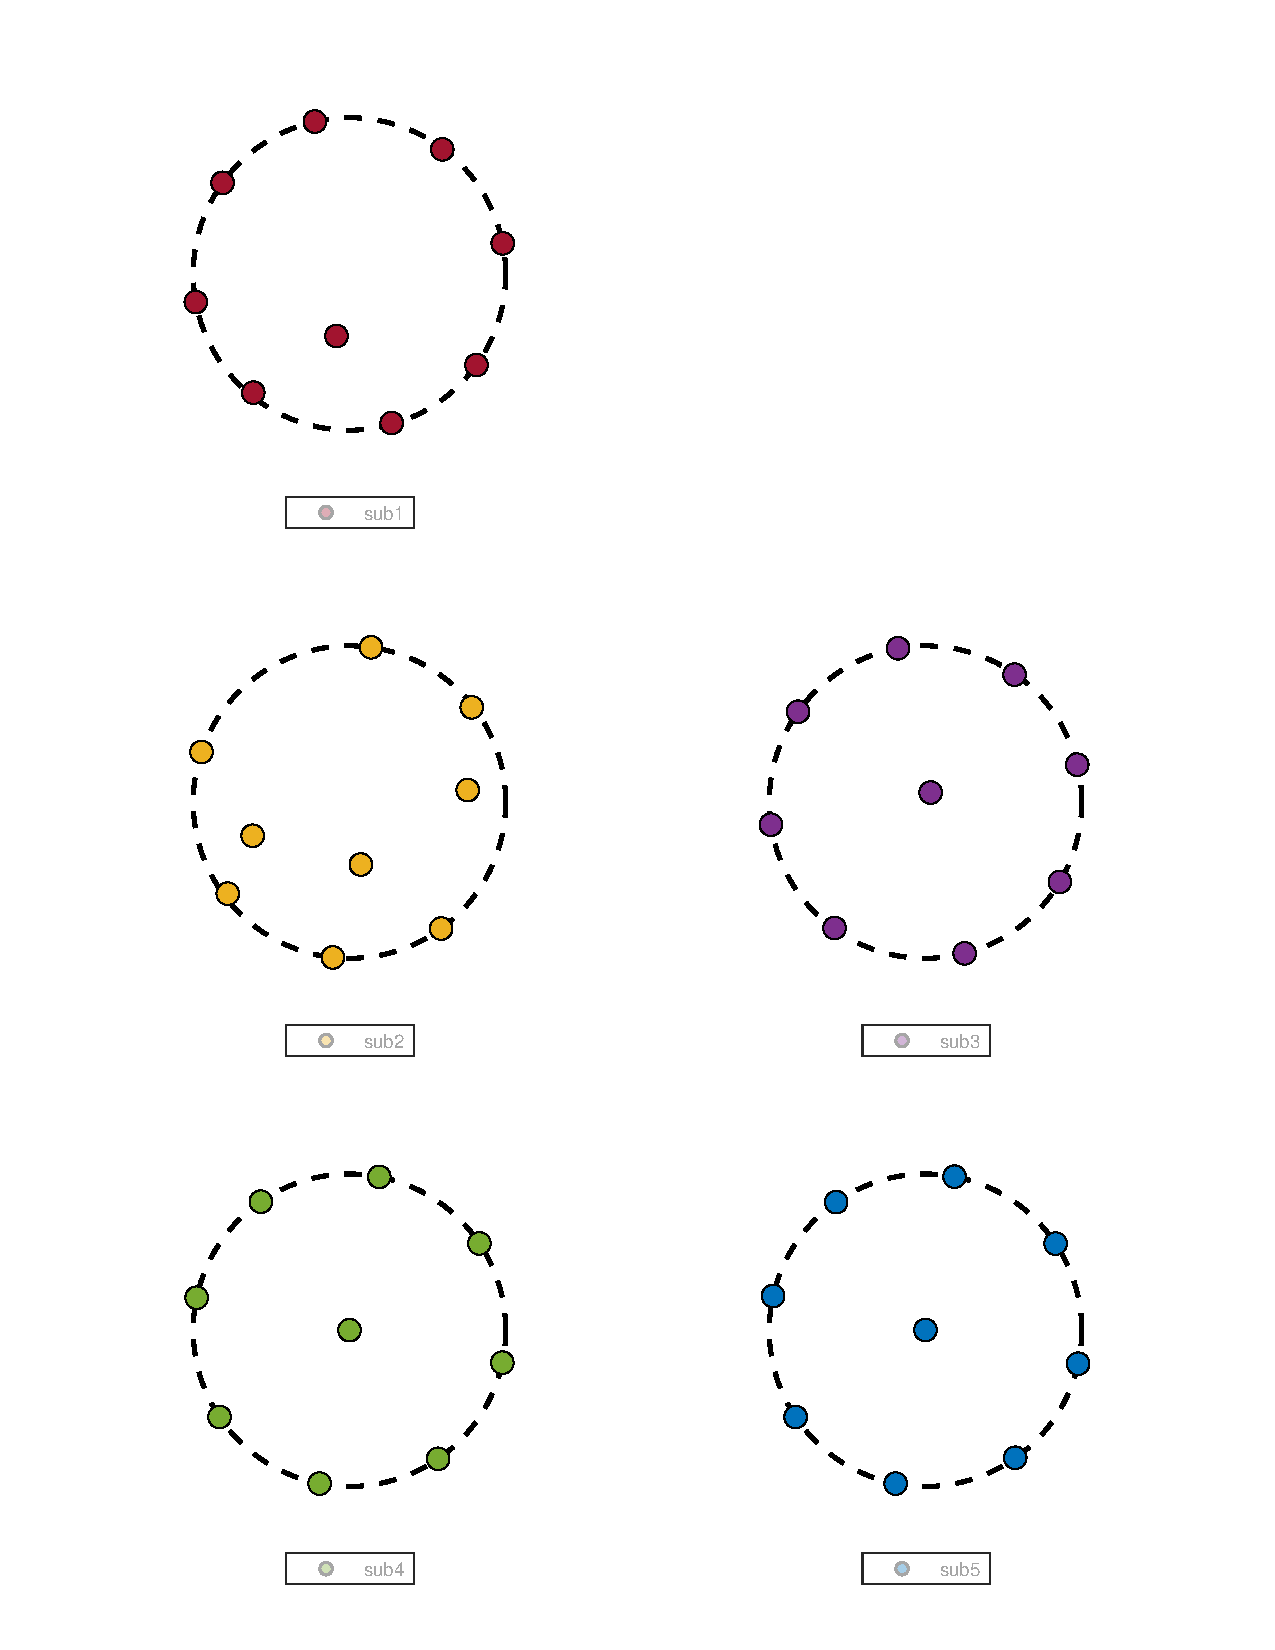
\includepdf[pages={-},scale=.8,pagecommand={\section*{Pictorial Representations of Case Study 1's Participant Submissions}\label{app:cs1-layouts}},linktodoc=true]{./figures/iea37-opt9-5plots.pdf}
% 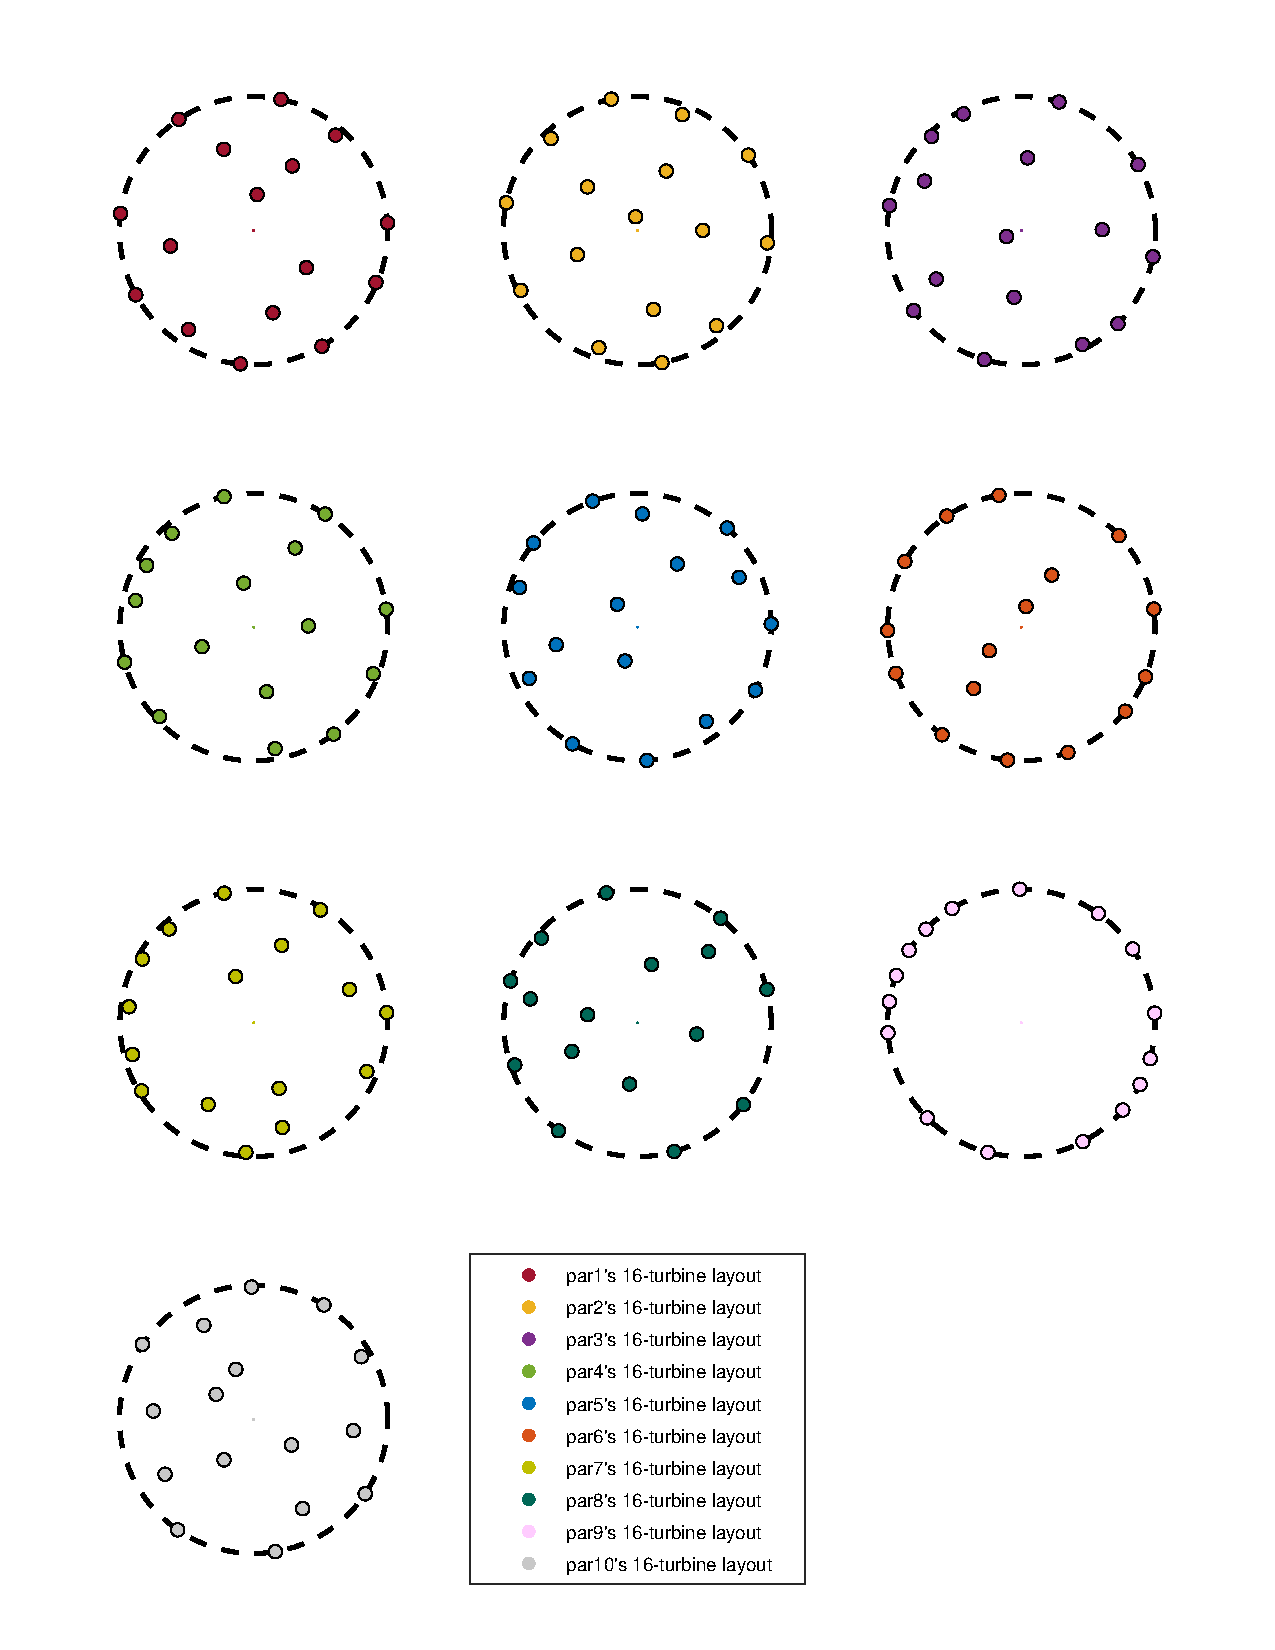
\includepdf[pages={-},scale=.8,pagecommand={\section*{Pictorial Representations of Case Study 2's 16-Turbine Submissions}\label{app:cs2-layouts1}},linktodoc=true]{./figures/iea37-opt16-10plots.pdf}
% 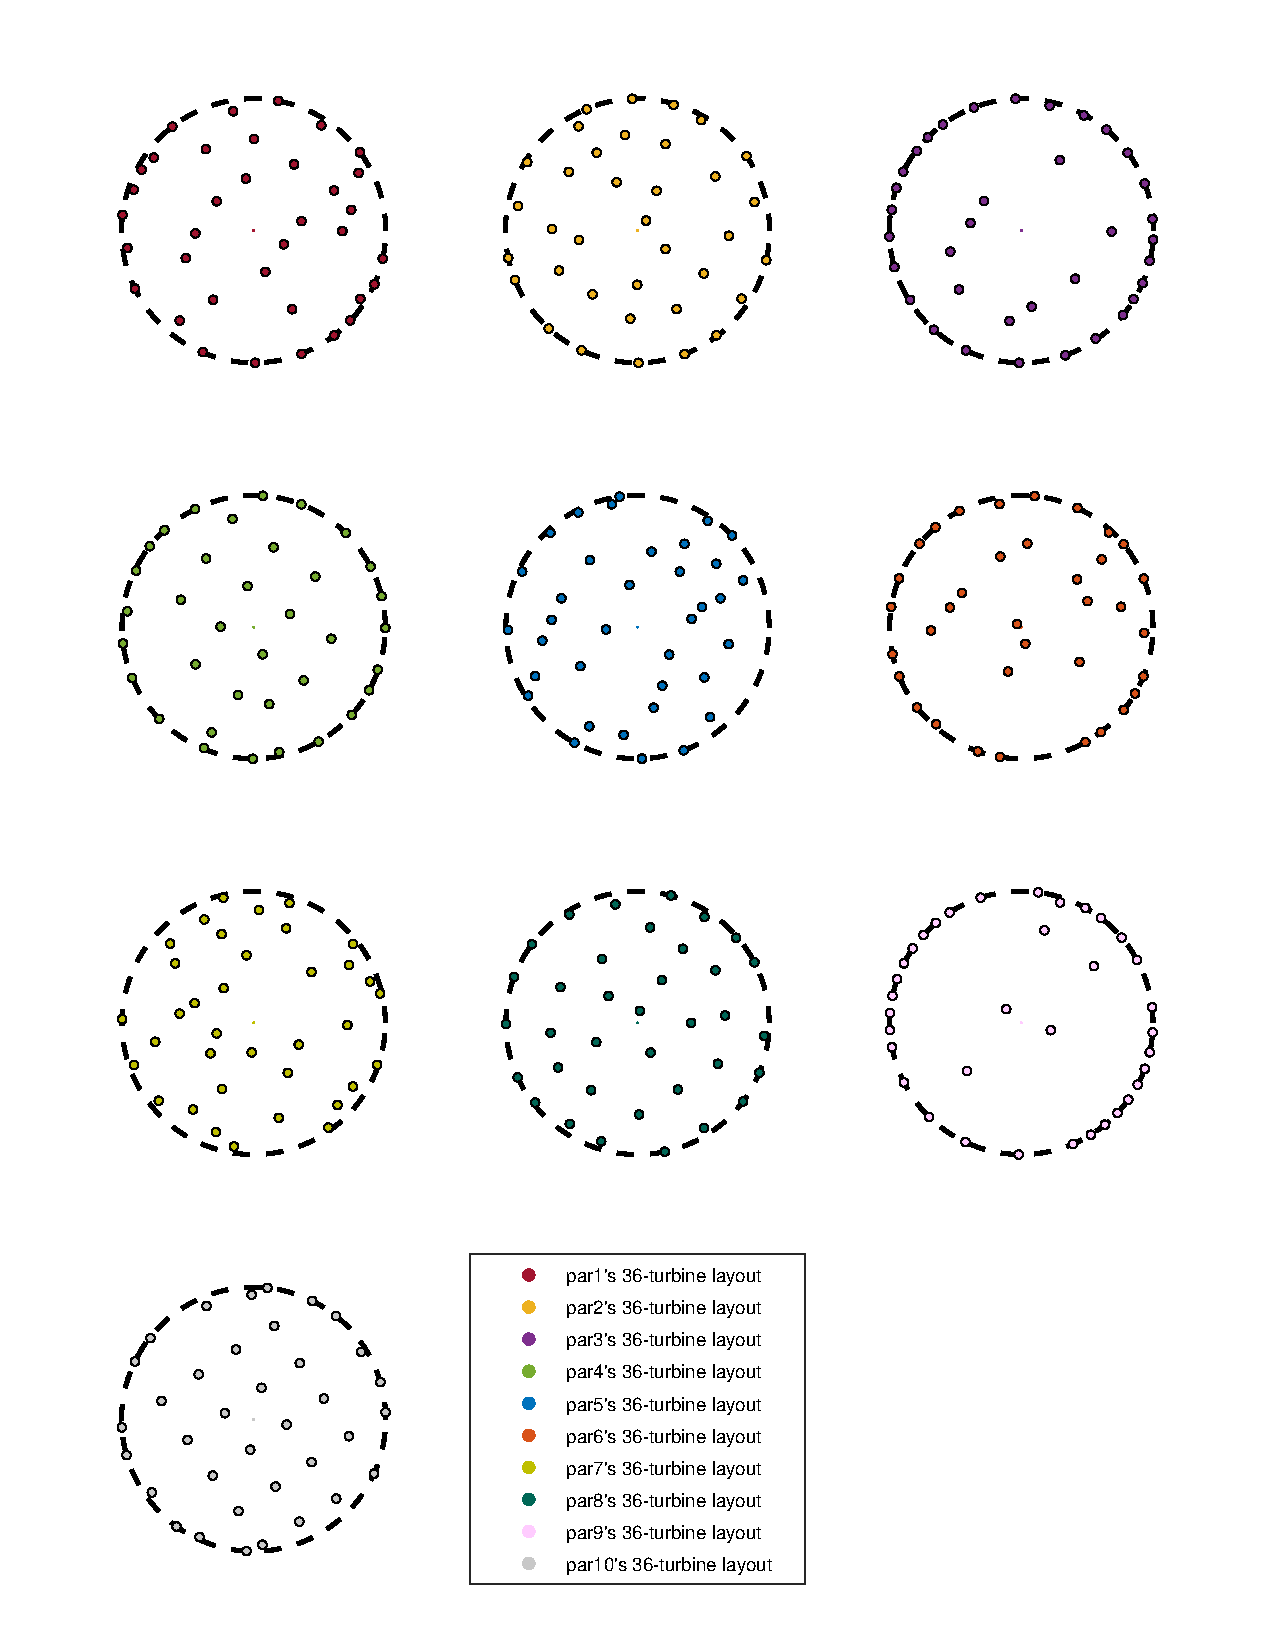
\includepdf[pages={-},scale=.8,pagecommand={\section*{Pictorial Representations of Case Study 2's 36-Turbine Submissions}\label{app:cs2-layouts2}},linktodoc=true]{./figures/iea37-opt36-10plots.pdf}
% 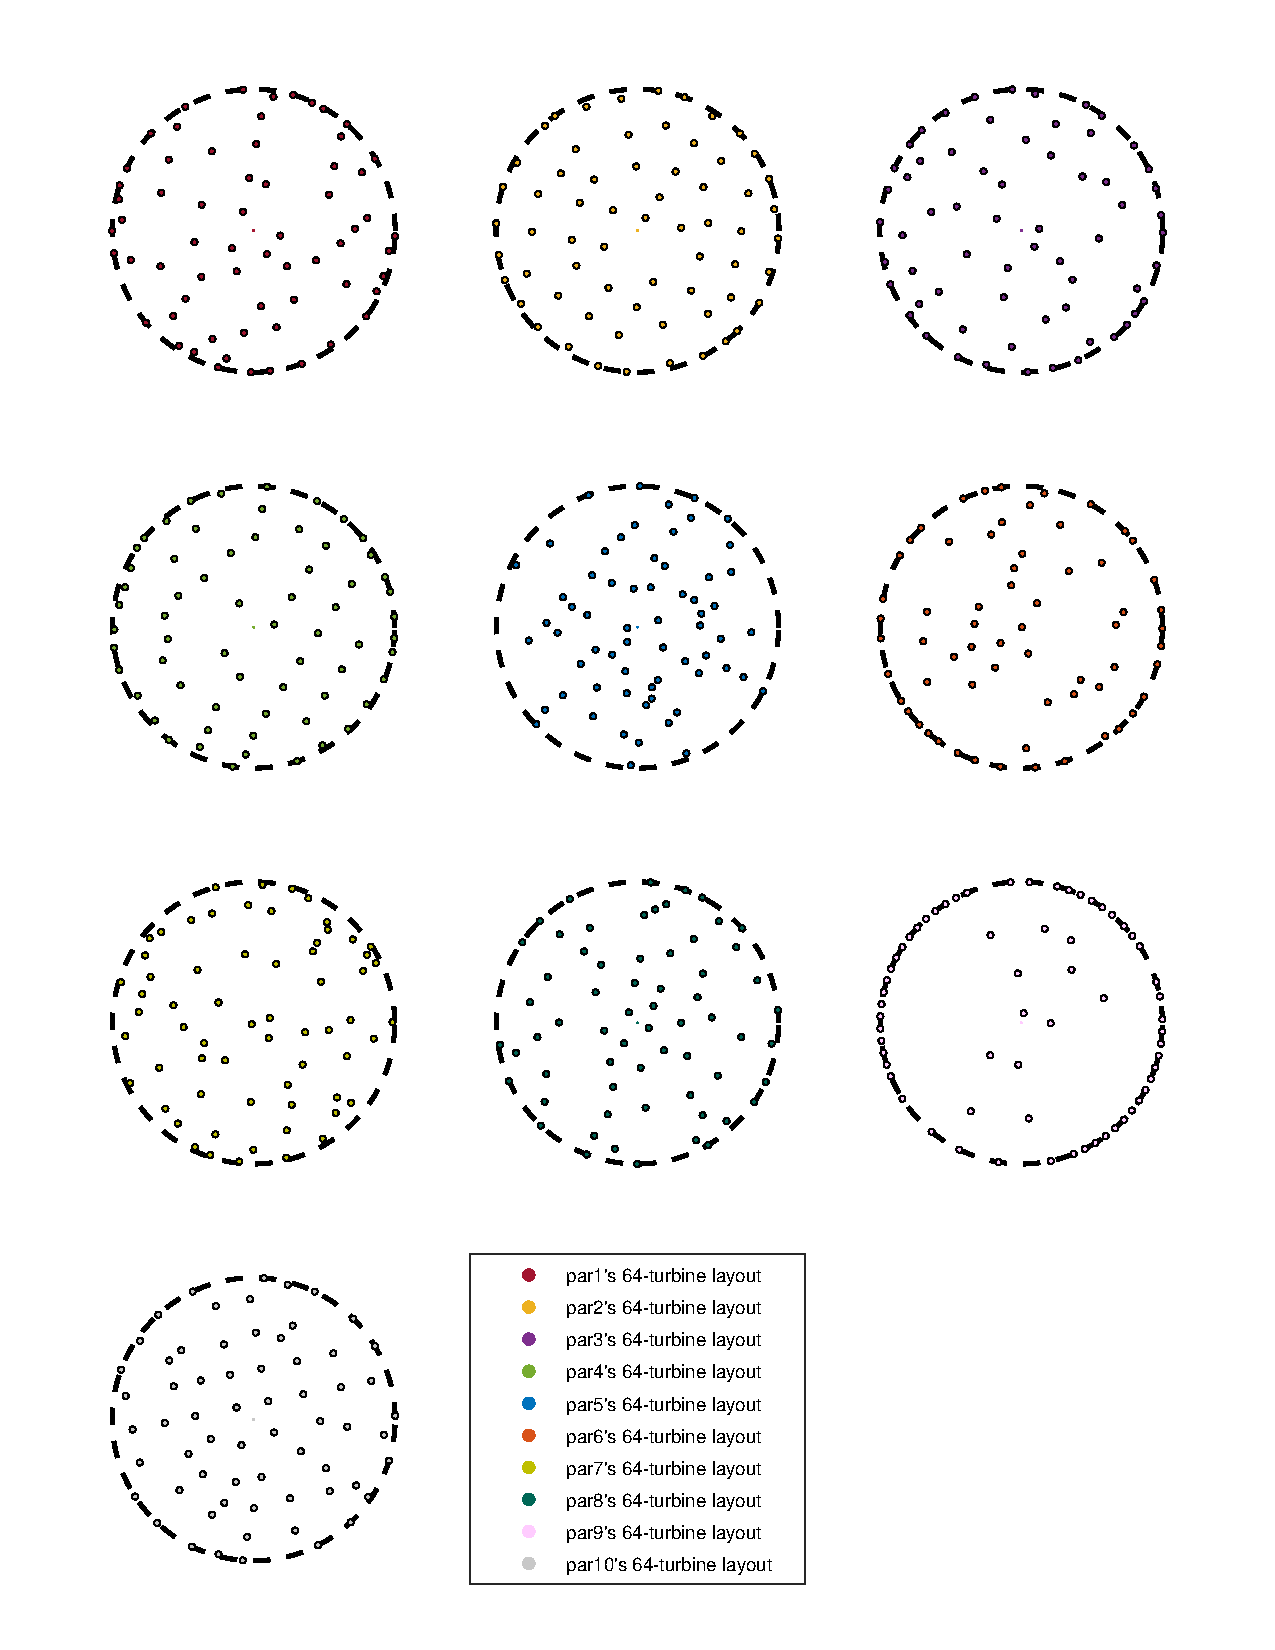
\includepdf[pages={-},scale=.8,pagecommand={\section*{Pictorial Representations of Case Study 2's 64-Turbine Submissions}\label{app:cs2-layouts3}},linktodoc=true]{./figures/iea37-opt64-10plots.pdf}
%\section{Python Code}
%\label{app:aepcalc}
%\lstinputlisting[language=python]{iea37-aepcalc.py}

\FloatBarrier

\pagebreak
%\bibliographystyle{new-aiaa}
\bibliography{aiaa-conf}
\end{document}